% -*- Mode:TeX -*-

%% IMPORTANT: The official thesis specifications are available at:
%%            http://libraries.mit.edu/archives/thesis-specs/
%%
%%            Please verify your thesis' formatting and copyright
%%            assignment before submission.  If you notice any
%%            discrepancies between these templates and the 
%%            MIT Libraries' specs, please let us know
%%            by e-mailing thesis@mit.edu

%% The documentclass options along with the pagestyle can be used to generate
%% a technical report, a draft copy, or a regular thesis.  You may need to
%% re-specify the pagestyle after you \include  cover.tex.  For more
%% information, see the first few lines of mitthesis.cls. 

%\documentclass[12pt,vi,twoside]{mitthesis}
%%
%%  If you want your thesis copyright to you instead of MIT, use the
%%  ``vi'' option, as above.
%%
%\documentclass[12pt,twoside,leftblank]{mitthesis}
%%
%% If you want blank pages before new chapters to be labelled ``This
%% Page Intentionally Left Blank'', use the ``leftblank'' option, as
%% above. 

\documentclass[12pt]{mitthesis}
\usepackage{lgrind}
\usepackage{amsmath}
\usepackage{multirow}
\usepackage{rotating}
\usepackage{cite}
\usepackage{subfigure}
\usepackage{lineno}
\pagestyle{plain}

%% This bit allows you to either specify only the files which you wish to
%% process, or `all' to process all files which you \include.
%% Krishna Sethuraman (1990).

\typein [\files]{Enter file names to process, (chap1,chap2 ...), or `all' to
process all files:}
\def\all{all}
\ifx\files\all \typeout{Including all files.} \else \typeout{Including only \files.} \includeonly{\files} \fi

\begin{document}


%% -*- Mode:TeX -*-
%
% Some departments (e.g. Chemistry) require an additional cover page
% with signatures of the thesis committee.  Please check with your
% thesis advisor or other appropriate person to determine if such a 
% page is required for your thesis.  
%
% If you choose not to use the "titlepage" environment, a \newpage
% commands, and several \vspace{\fill} commands may be necessary to
% achieve the required spacing.  The \signature command is defined in
% the "mitthesis" class
%
% The following sample appears courtesy of Ben Kaduk <kaduk@mit.edu> and
% was used in his June 2012 doctoral thesis in Chemistry. 

\begin{titlepage}
\begin{large}
This doctoral thesis has been examined by a Committee of the Department
of Chemistry as follows:

\signature{Professor Jianshu Cao}{Chairman, Thesis Committee \\
   Professor of Chemistry}

\signature{Professor Troy Van Voorhis}{Thesis Supervisor \\
   Associate Professor of Chemistry}

\signature{Professor Robert W. Field}{Member, Thesis Committee \\
   Haslam and Dewey Professor of Chemistry}
\end{large}
\end{titlepage}


%% -*-latex-*-
% 
% For questions, comments, concerns or complaints:
% thesis@mit.edu
% 
%
% $Log: cover.tex,v $
% Revision 1.8  2008/05/13 15:02:15  jdreed
% Degree month is June, not May.  Added note about prevdegrees.
% Arthur Smith's title updated
%
% Revision 1.7  2001/02/08 18:53:16  boojum
% changed some \newpages to \cleardoublepages
%
% Revision 1.6  1999/10/21 14:49:31  boojum
% changed comment referring to documentstyle
%
% Revision 1.5  1999/10/21 14:39:04  boojum
% *** empty log message ***
%
% Revision 1.4  1997/04/18  17:54:10  othomas
% added page numbers on abstract and cover, and made 1 abstract
% page the default rather than 2.  (anne hunter tells me this
% is the new institute standard.)
%
% Revision 1.4  1997/04/18  17:54:10  othomas
% added page numbers on abstract and cover, and made 1 abstract
% page the default rather than 2.  (anne hunter tells me this
% is the new institute standard.)
%
% Revision 1.3  93/05/17  17:06:29  starflt
% Added acknowledgements section (suggested by tompalka)
% 
% Revision 1.2  92/04/22  13:13:13  epeisach
% Fixes for 1991 course 6 requirements
% Phrase "and to grant others the right to do so" has been added to 
% permission clause
% Second copy of abstract is not counted as separate pages so numbering works
% out
% 
% Revision 1.1  92/04/22  13:08:20  epeisach

% NOTE:
% These templates make an effort to conform to the MIT Thesis specifications,
% however the specifications can change.  We recommend that you verify the
% layout of your title page with your thesis advisor and/or the MIT 
% Libraries before printing your final copy.
\title{An Optimizing Compiler for Low-Level Floating Point Operations}

\author{Lucien William Van Elsen}
% If you wish to list your previous degrees on the cover page, use the 
% previous degrees command:
%       \prevdegrees{A.A., Harvard University (1985)}
% You can use the \\ command to list multiple previous degrees
%       \prevdegrees{B.S., University of California (1978) \\
%                    S.M., Massachusetts Institute of Technology (1981)}
\department{Department of Electrical Engineering and Computer Science}

% If the thesis is for two degrees simultaneously, list them both
% separated by \and like this:
% \degree{Doctor of Philosophy \and Master of Science}
\degree{Bachelor of Science in Computer Science and Engineering}

% As of the 2007-08 academic year, valid degree months are September, 
% February, or June.  The default is June.
\degreemonth{June}
\degreeyear{1990}
\thesisdate{May 18, 1990}

%% By default, the thesis will be copyrighted to MIT.  If you need to copyright
%% the thesis to yourself, just specify the `vi' documentclass option.  If for
%% some reason you want to exactly specify the copyright notice text, you can
%% use the \copyrightnoticetext command.  
%\copyrightnoticetext{\copyright IBM, 1990.  Do not open till Xmas.}

% If there is more than one supervisor, use the \supervisor command
% once for each.
\supervisor{William J. Dally}{Associate Professor}

% This is the department committee chairman, not the thesis committee
% chairman.  You should replace this with your Department's Committee
% Chairman.
\chairman{Arthur C. Smith}{Chairman, Department Committee on Graduate Theses}

% Make the titlepage based on the above information.  If you need
% something special and can't use the standard form, you can specify
% the exact text of the titlepage yourself.  Put it in a titlepage
% environment and leave blank lines where you want vertical space.
% The spaces will be adjusted to fill the entire page.  The dotted
% lines for the signatures are made with the \signature command.
\maketitle

% The abstractpage environment sets up everything on the page except
% the text itself.  The title and other header material are put at the
% top of the page, and the supervisors are listed at the bottom.  A
% new page is begun both before and after.  Of course, an abstract may
% be more than one page itself.  If you need more control over the
% format of the page, you can use the abstract environment, which puts
% the word "Abstract" at the beginning and single spaces its text.

%% You can either \input (*not* \include) your abstract file, or you can put
%% the text of the abstract directly between the \begin{abstractpage} and
%% \end{abstractpage} commands.

% First copy: start a new page, and save the page number.
\cleardoublepage
% Uncomment the next line if you do NOT want a page number on your
% abstract and acknowledgments pages.
% \pagestyle{empty}
\setcounter{savepage}{\thepage}
\begin{abstractpage}
% $Log: abstract.tex,v $
% Revision 1.1  93/05/14  14:56:25  starflt
% Initial revision
% 
% Revision 1.1  90/05/04  10:41:01  lwvanels
% Initial revision
% 
%
%% The text of your abstract and nothing else (other than comments) goes here.
%% It will be single-spaced and the rest of the text that is supposed to go on
%% the abstract page will be generated by the abstractpage environment.  This
%% file should be \input (not \include 'd) from cover.tex.
In this thesis, I designed and implemented a compiler which performs
optimizations that reduce the number of low-level floating point operations
necessary for a specific task; this involves the optimization of chains of
floating point operations as well as the implementation of a ``fixed'' point
data type that allows some floating point operations to simulated with integer
arithmetic.  The source language of the compiler is a subset of C, and the
destination language is assembly language for a micro-floating point CPU.  An
instruction-level simulator of the CPU was written to allow testing of the
code.  A series of test pieces of codes was compiled, both with and without
optimization, to determine how effective these optimizations were.

\end{abstractpage}

% Additional copy: start a new page, and reset the page number.  This way,
% the second copy of the abstract is not counted as separate pages.
% Uncomment the next 6 lines if you need two copies of the abstract
% page.
% \setcounter{page}{\thesavepage}
% \begin{abstractpage}
% % $Log: abstract.tex,v $
% Revision 1.1  93/05/14  14:56:25  starflt
% Initial revision
% 
% Revision 1.1  90/05/04  10:41:01  lwvanels
% Initial revision
% 
%
%% The text of your abstract and nothing else (other than comments) goes here.
%% It will be single-spaced and the rest of the text that is supposed to go on
%% the abstract page will be generated by the abstractpage environment.  This
%% file should be \input (not \include 'd) from cover.tex.
In this thesis, I designed and implemented a compiler which performs
optimizations that reduce the number of low-level floating point operations
necessary for a specific task; this involves the optimization of chains of
floating point operations as well as the implementation of a ``fixed'' point
data type that allows some floating point operations to simulated with integer
arithmetic.  The source language of the compiler is a subset of C, and the
destination language is assembly language for a micro-floating point CPU.  An
instruction-level simulator of the CPU was written to allow testing of the
code.  A series of test pieces of codes was compiled, both with and without
optimization, to determine how effective these optimizations were.

% \end{abstractpage}

\cleardoublepage

\section*{Acknowledgments}

This is the acknowledgements section.  You should replace this with your
own acknowledgements.

%%%%%%%%%%%%%%%%%%%%%%%%%%%%%%%%%%%%%%%%%%%%%%%%%%%%%%%%%%%%%%%%%%%%%%
% -*-latex-*-

% Some departments (e.g. 5) require an additional signature page.  See
% signature.tex for more information and uncomment the following line if
% applicable.
\pagestyle{plain}
\bibliographystyle{unsrt}

\pagenumbering{roman}
  % -*- Mode:TeX -*-
%% This file simply contains the commands that actually generate the table of
%% contents and lists of figures and tables.  You can omit any or all of
%% these files by simply taking out the appropriate command.  For more
%% information on these files, see appendix C.3.3 of the LaTeX manual. 
\tableofcontents
\newpage
\listoffigures
\newpage
\listoftables



\pagenumbering{arabic}
\begin{linenumbers}
\chapter{Introduction and Theory Overview}

\section{Introduction}
This thesis presents the analysis details and the results of the search for heavy resonances decaying into a $Z$ boson and a Higgs boson (h) at the center-of-mass energy of 8 TeV, using 19.7 fb$^{-1}$ p-p collision data. In turn, the $Z$ boson is identified through its leptonic decays (leptons often refer to $e$ and $\mu$ only in experiments. $l = e, \mu$). The Higgs boson h is expected to hadronically decay into a pair of b-quarks. The investigated final states consist of two charged leptons which are identified in the detector and limit the presence of the background, and two b-quarks from the hadronic Higgs decay which collects the largest possible fraction of Higgs events.
\newline This thesis is organised as follows. In the latter part of this chapter, the model that predicts heavy resonances is introduced, including the expected cross section and the specification of model parameters. In chapter 2, the LHC and the CMS experiment are described, including the information of each sub-detector and the trigger system of the CMS. The details of the analysis are shown in chapter 3. This chapter reveals the way to reconstruct physical objects in CMS. By adding some proper kinematic selections on those physics objects, the interested events in data collected by the CMS detector can be selected. Moreover, this chapter shows the comparison between data and simulation. In the last chapter, the results of the search and the conclusion are presented.

\section{Theory Overview}
Although the Higgs boson discovered by the ATLAS and CMS collaborations\cite{atlas-higgs-1,cms-higgs-1,cms-higgs-2} imposes strong constraints on theories beyond the Standard Model(SM), the extreme fine tuning in quantum corrections required to have a light fundamental Higgs boson with mass close to 125 GeV\cite{cms-higgs-3,atlas-higgs-2,atlas-higgs-3,atlas-cms-higgs} suggests that the Standard Model may be incomplete, and not valid beyond a scale of a few TeV. Various dynamical electroweak symmetry breaking scenarios which attempt to solve this naturalness problem, such as Minimal Walking Technicolor\cite{technicolor}, Little Higgs\cite{little-higgs-1,little-higgs-2,little-higgs-3}, or composite Higgs models\cite{compositehiggs-1,compositehiggs-2,compositehiggs-3} predict the existence of new resonances decaying to a vector boson plus a Higgs boson.

\subsection{Heavy Vector Triplet Model}
Resonance searches are typically not sensitive to all the details and the free parameters of the underlying model, but only to those parameters or combinations of parameters that control the mass of the resonance and the interactions involved in its production and decay. Therefore, one can employ a simplified description of the resonance defined by a phenomenological Lagrangian where only the relevant couplings and mass parameters are retained. This model-independent strategy applies a Heavy Vector Triplet (HVT)\cite{HVT} to the Standard Model group and reproduces a large class of explicit models. In Eq.~(\ref{eq:phen-Lag}), the mathematical form of the simplified Lagrangian is defined, where $V_{\nu}^{a}$ , $a$ = 1,2,3, is a real vector with vanishing hypercharge in the adjoint representation of $SU(2)_{L}$, it decscribes one charged and one neutral heavy spin-1 particle with charge eigenstate fields, and $D_{[\mu}V_{\nu]}^{a}$ represents the covariant derivative.

\begin{align} 
  \label{eq:phen-Lag}
  \mathcal{L}_{\mathcal{V}} =& -\frac{1}{4}D_{[\mu}V_{\nu]}^{a}D^{[\mu}V^{\nu] a}+\frac{{m_{V}^{2}}}{2}V_{\mu}^{a}V^{\mu a}\nonumber\\&+ig_{V}c_{H}V_{\mu}^{a}H^{\dagger}{\tau}^{a}{\overset{\text{\scriptsize$\leftrightarrow$}}{D}}^{\mu}H+\frac{g^{2}}{g_{V}}c_{F}V_{\mu}^{a}\sum_{f}\bar{f}_{L}{\gamma}^{\mu}{\tau}^{a}f_{L}\nonumber\\&+\frac{g_{V}}{2}c_{VVV}\epsilon_{abc}V_{\mu}^{a}V_{\nu}^{b}D^{[\mu}V^{\nu] c}+\textup{quadrilinear terms}
\end{align}

\begin{align}
  V_{\mu}^{\pm}=\frac{V_{\mu}^{1}\mp iV_{\mu}^{2}}{\sqrt{2}}\textup{ , }V_{\mu}^{0}=V_{\mu}^{3}
\end{align}
\begin{align}
  D_{[\mu}V_{\nu]}^{a} = D_{\mu}V_{\nu}^{a}-D_{\nu}V_{\mu}^{a}\textup{ , }D_{\mu}V_{\nu}^{a}=\partial_{\mu}V_{\nu}^{a}+g\epsilon^{abc}W_{\mu}^{b}V_{\nu}^{c}
\end{align}
\newline In these models, new heavy vector bosons ($V^{\pm}, V^{0}$) that couple to the Higgs and SM gauge bosons with the parameters $c_{H}$ and $g_{V}$ and to the fermions via the combination $(g^{2}/g_{V})c_{F}$ . The parameter $g_{V}$ represents the strength of the new vector boson interaction, while $c_{H}$ and $c_{F}$ represent the couplings to the Higgs and the fermions respectively, and are expected to be of the order of unity in most models. 


\subsection{Basic Phenomenology}
\subsection*{Masses and Mixings}
After electro-weak symmetry breaking (EWSB), the only massless state is photon, which can be identified as the gauge field associated with the unbroken $U(1)_{em}$. The two other neutral mass eigenstates are the SM $Z$ boson and one heavy vector of mass $M_{0}$ which are obtained by diagonalizing the mass matrix of the ($Z,V^{0}$) system by a rotation with angle $\theta_{N}$
\begin{align}
  \begin{pmatrix}
    Z\\
    V^{0}
  \end{pmatrix}
  \rightarrow
  \begin{pmatrix}
    \cos{\theta_{N}} & \sin{\theta_{N}}\\
    -\sin{\theta_{N}}& \cos{\theta_{N}}
  \end{pmatrix}
  \begin{pmatrix}
    Z\\
    V^{0}
  \end{pmatrix}
  .
\end{align}
The mass matrix is
\begin{align}
  \label{eq:MassMatrixN}
  \mathcal{M}_{N}^{2}=
  \begin{pmatrix}
    \hat{m}_{Z}^{2} & c_{H}\xi \hat{m}_{Z} \hat{m}_{V}\\
    c_{H}\xi \hat{m}_{Z} \hat{m}_{V} & \hat{m}_{V}^{2}
  \end{pmatrix}
  \textup{ , where}
  \begin{cases}
    \hat{m}_{Z}=\frac{e\hat{\upsilon}}{2\sin{\theta_{W}}\cos{\theta_{W}}}\\
    \hat{m}_{V}^{2}=m_{V}^{2}+g_{V}^{2}c_{VVHH}\hat{\upsilon}^{2}\\
    \xi=\frac{g_{V}\hat{\upsilon}}{2\hat{m}_{V}}
  \end{cases}
  .
\end{align}
In the above equations $\hat{\upsilon}$ denotes the Vacuum Expetation Value (VEV) defined by $\big \langle H^{\dagger}H\big \rangle=\hat{\upsilon}^{2}/2$, and one should know the masses $\hat{m}_{Z}$ and $\hat{m}_{V}$ do not coincide with the physical $Z$ boson and the masses of the new resonances of this model, although they do in the approximations later. The mass eigenvalues and the rotation angles are easily obtained by inverting the relations
\begin{align}
  \label{eq:detMN}
  &Tr[\mathcal{M}_{N}^{2}]=\hat{m}_{Z}^{2}+\hat{m}_{V}^{2}=m_{Z}^{2}+M_{0}^{2}\textup{ ,}\nonumber\\
  &Det[\mathcal{M}_{N}^{2}]=\hat{m}_{Z}^{2}\hat{m}_{V}^{2}(1-c_{H}^{2}\xi^{2})=m_{Z}^{2}M_{0}^{2}\textup{ ,}\nonumber\\
  &\tan{2\theta_{N}}=\frac{2c_{H}\xi \hat{m}_{Z} \hat{m}_{V}}{\hat{m}_{V}^{2}-\hat{m}_{Z}^{2}}\textup{ .}
\end{align}
Notice that the tangent can be uniquely inverted because the angle $\theta_{N}$ is in the range $[-\pi/4,\pi/4]$ in the parameter region we will be interested in, where $\hat{m}_{Z}<\hat{m}_{V}$.
\newline The situation is similar in the charged vector where the mass matrix of the ($W^{\pm},V^{\pm}$) system reads
\begin{align}
  \label{eq:MassMatrixC}
  \mathcal{M}_{C}^{2}=
  \begin{pmatrix}
    \hat{m}_{W}^{2} & c_{H}\xi \hat{m}_{W} \hat{m}_{V}\\
    c_{H}\xi \hat{m}_{W} \hat{m}_{V} & \hat{m}_{V}^{2}
  \end{pmatrix}
  \textup{ , where }
  \hat{m}_{W}=\frac{e\hat{\upsilon}}{2\sin{\theta_{W}}}=\cos{\theta_{W}}\hat{m}_{Z}
  \textup{ ,}
\end{align}
and it is diagonalized by
\begin{align}
  \label{eq:detMC}
  &Tr[\mathcal{M}_{C}^{2}]=\hat{m}_{W}^{2}+\hat{m}_{V}^{2}=m_{W}^{2}+M_{\pm}^{2}\textup{ ,}\nonumber\\
  &Det[\mathcal{M}_{C}^{2}]=\hat{m}_{W}^{2}\hat{m}_{V}^{2}(1-c_{H}^{2}\xi^{2})=m_{W}^{2}M_{\pm}^{2}\textup{ ,}\nonumber\\
  &\tan{2\theta_{C}}=\frac{2c_{H}\xi \hat{m}_{W} \hat{m}_{V}}{\hat{m}_{V}^{2}-\hat{m}_{W}^{2}}\textup{ .}
\end{align}
By checking Eq.~(\ref{eq:MassMatrixN}) and Eq.~(\ref{eq:MassMatrixC}), the charged and neutral mass matrices are connected by custodial symmetry, which can be shown in full generality to imply
\begin{align}
  \mathcal{M}_{C}^{2}=
  \begin{pmatrix}
    \cos{\theta_{W}} & 0\\
    0&1
  \end{pmatrix}
  \mathcal{M}_{N}^{2}
  \begin{pmatrix}
    \cos{\theta_{W}} & 0\\
    0&1
  \end{pmatrix}
  \textup{ .}
\end{align}
By taking the determinant of the above equation, or equivalently by comparing the charged and neutral determinants in Eq.~(\ref{eq:detMN}) and Eq.~(\ref{eq:detMC}), we obtain a generalized custodial relation among the physical masses
\begin{align}
  \label{eq:custRelation}
m_{W}^{2}M_{\pm}^{2}=\cos^{2}\theta_{W}m_{Z}^{2}M_{0}^{2}\textup{ .}
\end{align}
From the simple formula above, we can start to identify the physically reasonable region of the parameter space in this model. We aim at describing new vectors with masses at or above the TeV scale, but we also want the SM masses $m_{W,Z} \sim$ 100 GeV to be reproduced. Therefore we require a hierachy in the mass relation of SM $Z$ and $W$ bosons versus the new vectors.
\begin{align}
  \label{eq:hierachyEq}
  \frac{\hat{m}_{W,Z}}{\hat{m}_{V}}\sim \frac{m_{W,Z}}{M_{\pm ,0}}\leq10^{-1}\ll1
\end{align}
In the limit of Eq.~(\ref{eq:hierachyEq}) we obtain simple approximation for $m_{W}$ and $m_{Z}$
\begin{align}
  &m_{Z}^{2}=\hat{m}_{Z}^{2}(1-c_{H}^{2}\xi^{2})(1+\mathcal{O}(\hat{m}_{Z}^{2}/\hat{m}_{V}^{2}))\textup{ ,}\nonumber\\
  &m_{W}^{2}=\hat{m}_{W}^{2}(1-c_{H}^{2}\xi^{2})(1+\mathcal{O}(\hat{m}_{W}^{2}/\hat{m}_{V}^{2}))\textup{ .}
\end{align}
The parameter $\xi$ can be either very small or of order unity. Both cases are realized in explicit models. While $\xi\ll1$ is the most common situation, $\xi\sim1$ only occurs in strongly coupled scenarios at very large $g_{V}$. In these approximations, SM tree-level experimental observation can be reproduced to percent accuracy.
\newline Since $\hat{m}_{W}=\cos\theta_{W}\hat{m}_{Z}$, the $W$-$Z$ mass ratio is thus given by
\begin{align}
  \label{eq:fracWZ}
  \frac{m_{W}^{2}}{m_{Z}^{2}}\simeq \cos^{2}{\theta_{W}}\textup{ .}
\end{align}
Eq.~(\ref{eq:fracWZ}) has one important implication on the masses of the new vectors. When combined with the custodial relation Eq.~(\ref{eq:custRelation}), it tells us that the charged and neutral $V$s are practically degenerate
\begin{align}
  M_{\pm}^{2}=M_{0}^{2}(1+\mathcal{O}(\%))\textup{ ,}
\end{align}
In the following, when working at the leading order in the limit Eq.~(\ref{eq:hierachyEq}), we can ignore the mass splitting and denote the mass of the charged and the neutral states collectively as $M_{V}$. It is easy to check that in that limit $M_{V}=\hat{m}_{V}$.

\subsection*{Decay Widths}
Because of the hierachy in the mass matrices, the mixing angles are naturally small. By looking at Eqs.~(\ref{eq:detMN}), (\ref{eq:detMC}) and (\ref{eq:hierachyEq}) we can estimate
\begin{align}
  \theta_{N,C}\simeq c_{H}\xi \frac{\hat{m}_{W,Z}}{\hat{m}_{V}}\leq10^{-1}\textup{ ,}
\end{align}
and after rotating to the mass basis, the coupling of the neutral and charged resonances to left- and right-handed fermion chiralities can be written in a compact form for each fermion species $F=\{l,q,3\}$.
\begin{align}
\begin{cases}  
  g_{L}^{N}=\frac{g^{2}}{g_{V}}\frac{c_{F}}{2}\cos\theta_{C}+(g_{L}^{Z})_{SM}\sin\theta_{N}\simeq\frac{g^{2}}{g_{V}}\frac{c_{F}}{2}\textup{ ,}\\
  g_{R}^{N}=(g_{R}^{Z})_{SM}\sin\theta_{N}\simeq0
\end{cases}\nonumber\\
\begin{cases}
  g_{L}^{C}=\frac{g^{2}}{g_{V}}\frac{c_{F}}{2}\cos\theta_{C}+(g_{L}^{W})_{SM}\sin\theta_{C}\simeq\frac{g^{2}}{g_{V}}\frac{c_{F}}{2}\textup{ ,}\\
  g_{R}^{C}=0
\end{cases}
\end{align}
In the above equation $(g_{L,R}^{W,Z})_{SM}$ denote the ordinary SM $W$ and $Z$ couplings (with the normalization given by $g_{L}^{W}=g/\sqrt{2}$).\\
\newline Given that the rotation angles are small, the couplings further simplify, as also shown in the equation. We could see that $V$ interact mainly with left-handed chiralities and that all the couplings for each fermion species are controlled by the parameter combination $g^{2}/g_{V}c_{F}$. This gives tight correlations among different channels
\begin{align}
  \label{eq:DRfermion}
  \Gamma_{V_{\pm}\rightarrow f\bar{f}'}\simeq2\Gamma_{V_{0}\rightarrow f\bar{f}'}\simeq N_{C}[f](\frac{g^{2}c_{F}}{g_{V}})^{2}\frac{M_{V}}{48\pi}\textup{ ,}
\end{align}
where $N_{C}[f]$ is the number of colors (3 for the di-quark and 1 for the dilepton decays). The parameters $c_{F}=\{c_{l},c_{q},c_{3}\}$ control the relative BRs to leptons, light quarks and the third family.
\newline In the case of di-boson decay width
\begin{align}
  \label{eq:DRboson}
  &\Gamma_{V_{0}\rightarrow W_{L}^{+}W_{L}^{-}}\simeq\Gamma_{V_{\pm}\rightarrow W_{L}^{\pm}Z_{L}}\simeq\frac{g_{V}^{2}c_{H}^{2}M_{V}}{192\pi}\frac{(1+c_{H}c_{VVV}\xi^{2})^{2}}{(1-c_{H}^{2}\xi^{2})^{2}}=\frac{g_{V}^{2}c_{H}^{2}M_{V}}{192\pi}[1+\mathcal{O}(\xi^{2})]\textup{ ,}\nonumber\\
  &\Gamma_{V_{0}\rightarrow Z_{L}h}\simeq\Gamma_{V_{\pm}\rightarrow W_{L}^{\pm}h}\simeq\frac{g_{V}^{2}c_{H}^{2}M_{V}}{192\pi}\frac{(1-4c_{VVHH}\xi^{2})^{2}}{1-c_{H}^{2}\xi^{2}}=\frac{g_{V}^{2}c_{H}^{2}M_{V}}{192\pi}[1+\mathcal{O}(\xi^{2})]\textup{ .}\nonumber\\
\end{align}
Note that Eq.~(\ref{eq:DRboson}) is derived in the Equivalent Gauge\cite{EquivGauge} because the decay to transverse SM vectors is highly suppressed while to the longitudinal parts grows with the energy of the process, therefore the Unitary Gauge which is used in the original Lagrangian is instead useful. The channels that are not shown in the above equations are either forbidden, like $hh$ and $\gamma\gamma$ decays, or suppressed like the decays to transverse polarizations.
\newline From this section, a very simple picture emerges. At small $\xi$, all the decay widths are fixed with a given resonance mass $M_{V}$ and the couplings $\{g^{2}c_{F}/g_{V}$, $g_{V}c_{H}\}$ which control the BRs in all relevant channels. Paremeters $c_{VVV},\textup{ } c_{VVHH}\textup{ and }c_{VVW}$ are basically irrelevent. Thus, the basic phenomenology of this model is well described by a good approximation.


\newpage
\subsection{Explicit Models}
Now the general picture is clear, we can get exact values of the widths and BRs from explicit models. Consider two benchmark models, A and B, which correspond to two explicit models describing the heavy vectors in Refs.~\cite{modelA} and \cite{compositehiggs-1} respectively. All the $c$ parameters are fixed to specific values in these models and the only free parameters are the resonance mass $M_{V}$ and coupling $g_{V}$. Moreover, model A is inspired by weakly coupled extensions of the SM gauge group while model B is by strongly coupled scenarios of EWSB, $i.e.$ Composite Higgs models, we will consider them in different regions of $g_{V}$, relatively small $g_{V}\leq3$ and relatively large $g_{V}\geq3$.\\
\newline Figure \ref{fig:BRs_AvsB} shows the BRs as functions of the mass in model A and B. As expected from the previous discussion and according to Refs.~\cite{modelA}, model A predicts
\begin{align}
  \label{eq:DeterA}
  &c_{H}=-g^{2}/g_{V}^{2}\textup{ , }c_{F}\simeq 1 \textup{ ,} \nonumber\\
  &|g_{V}c_{H}|\simeq g^{2}c_{F}/g_{V}\simeq g^{2}/g_{V}\textup{ .}
\end{align}
Therefore Eq.~(\ref{eq:DRfermion}) and (\ref{eq:DRboson}) can be determined in the following form for $V_{0}$ in model A ($g_{V}=1$),
\begin{align}
  &\Gamma_{V_{0}\rightarrow f\bar{f}'}\simeq N_{c}[f]\frac{g^{4}M_{V}}{96\pi}\nonumber\\
  &\Gamma_{V_{0}\rightarrow W^{+}W^{-}}\simeq \Gamma_{V_{0}\rightarrow Zh}\simeq \frac{g^{4}M_{V}}{192\pi}\textup{ .}
\end{align}
One can easily check either from the plot or the equation, a factor of two difference comparing the BRs between fermions and bosons. Due to the color factor, leptons and quarks also have a difference by a factor of three. Since the $c_{F}$ term is universal both in A and B. The total width in model A decreases with increasing $g_{V}$ because of the overall suppresion ($g^{2}/g_{V}$) in Eq.~(\ref{eq:DeterA}).\\On the contrary, in model B the $c_{H}$ term is unsuppressed
\begin{align}
  \label{eq:DeterB}
  &c_{H}\simeq c_{F}\simeq 1 \textup{ ,}\nonumber\\
  &g_{V}c_{H}\simeq-g_{V}\textup{ , }g^{2}c_{c_{F}}/g_{g_{V}}\simeq g^{2}/g_{V}\textup{ .}
\end{align}
Thus the determinate $V_{0}$ decay widths for model B ($g_{V}=3$) are
\begin{align}
  &\Gamma_{V_{0}\rightarrow f\bar{f}'}\simeq N_{c}[f]\frac{g^{4}M_{V}}{342\pi}\nonumber\\
  &\Gamma_{V_{0}\rightarrow W^{+}W^{-}}\simeq \Gamma_{V_{0}\rightarrow Zh}\simeq \frac{3M_{V}}{64\pi}\textup{ .}
\end{align}
For model B$_{g_{V}=3}$ the dominant BRs are into di-bosons and the fermionic decays are extremely suppressed. Moreover, the total width increases with increasing $g_{V}$ since it is dominated by the di-boson width which grows with $g_{V}$ as expected from Eq.~({\ref{eq:DeterB}}). This model B is particularly interesting for the present search, since it predicts signal cross sections in order of fb\cite{HVT} \cite{CMS_AN_2015-186}, branching ratios to vector bosons close to unity, and thus being accessible at the LHC. In the latter chapters, the mass eigenstate of the neutral heavy vector boson in model B scenario refers to the $Z'$ particle, which is the search target of this thesis.\\
\begin{figure}[h]
  \begin{center}
    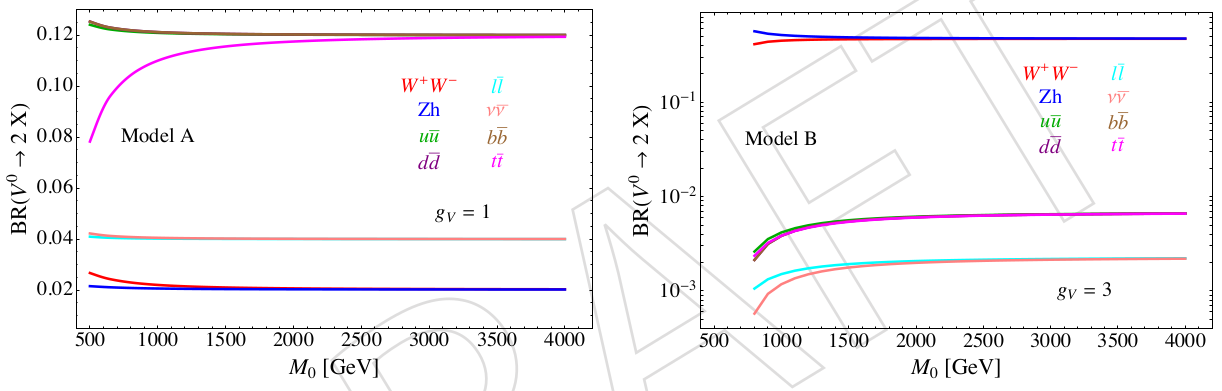
\includegraphics[width=\textwidth]{figure/CH1/BRs_modelAvsB.png}
  \end{center}
  \caption{\label{fig:BRs_AvsB}Branching ratios as a function of the resonance mass for the HVT benchmark model A(left) and model B(right).}
\end{figure}

\chapter{CMS detector and LHC}
This thesis is done via analyzing the data collected by the Compact Muon Solenid (CMS) detector at the Large Hadron Collider (LHC). CMS is one of the two largest detectors built on the LHC. This chapter will briefly introduce the LHC and the CMS detector.

\section{Large Hadron Collider}
The LHC is the world's most powerful hadron collider and the largest experimental facility ever. It was built by the European Organization for Nuclear Research (CERN) between 1998 and 2008 in collaboration with over 10,000 scientists and engineers from over 100 countries, as well as hundreds of universities and laboratories. It lies in a tunnel 27 km in circumference, as deep as 175 m beneath the France$-$Switzerland border near Geneva. The designed maximum collison energy and highest luminosity of the LHC are 14 TeV and $\textup{10}^{-34} \textup{cm}^{-2}\textup{s}^{-1}$ respectively.

Other accelerators that had been originally built at CERN for previous experiments is working as an injection chain for the LHC now. The proton beam starts from LINAC, a small linear accelerator, where its energy firstly reaches 50 MeV. It then passes through a booster and goes to the PS, where it is accelerated up to 25 GeV. After that, it reaches 450 GeV in the SPS. The beam is finally injected in the LHC ring from the SPS, it is accelerated up to 4 TeV in 2012. In early 2015, the proton beam had been acceletated to 6.5 TeV, a value near its designed energy, before undergoing collision.

There are four collision points at the LHC, corresponding to four main experiments, CMS, ATLAS, LHCb and ALICE. The ALICE experiment is optimized to study heavy-ion (Pb-Pb nuclei) collisions and focusing on the physics of strongly interacting matter at extreme energy densities. LHCb is a specialized b-physics experiment, measuring the parameters of CP violation in the interactions of b-hadrons. Such studies can help to explain the matter-antimatter asymmetry of the universe. Last, CMS and ATLAS are two general purpose detectors. The aims of these two experiments are investigating a wide range of physics, including the search for the beyond standard model particles, extra dimensions, and dark matter.


\begin{figure}[hbtp]
  \begin{center}
    \includegraphics[width=0.9\textwidth]{figure/CH2/CERN_Overview.jpg}
  \end{center}
  \caption{\label{fig:LHC_overview}Overview of the LHC and relative location of the detectors.}
\end{figure}

\begin{figure}[hbtp]
  \begin{center}
    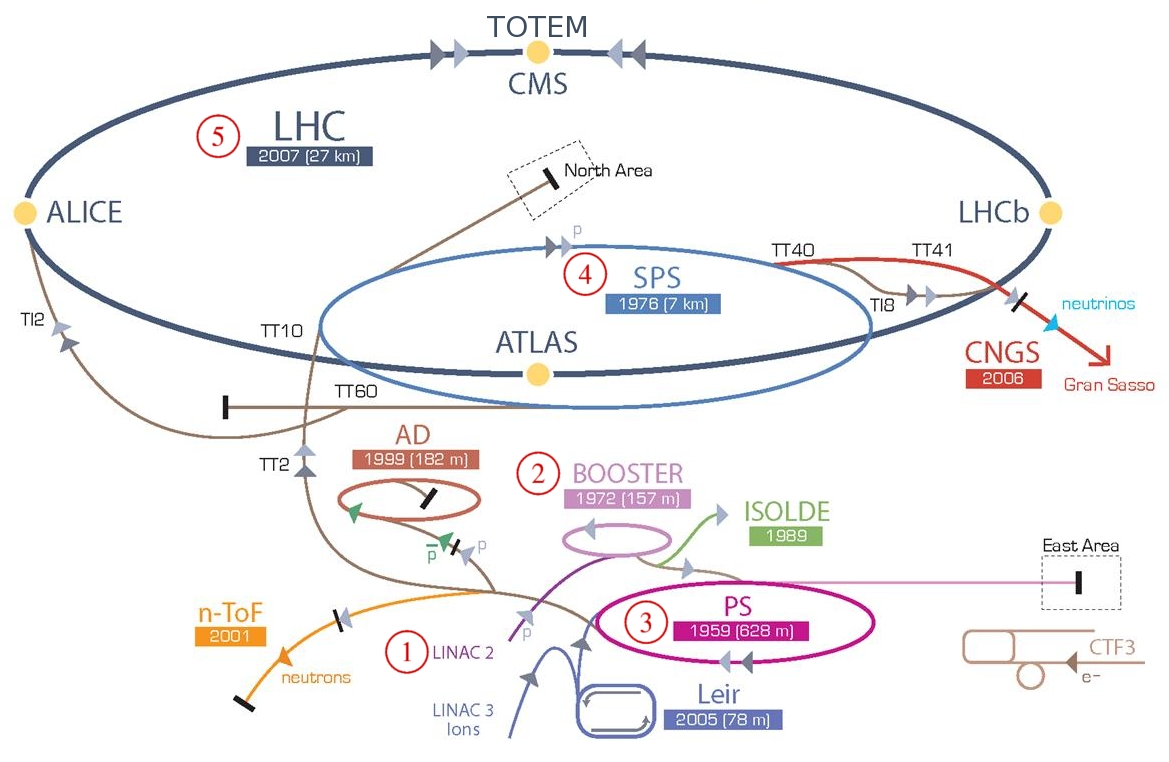
\includegraphics[width=0.9\textwidth]{figure/CH2/complex.png}
  \end{center}
  \caption{\label{fig:accelerator}CERN accelerator complex.}
\end{figure}

\section{Compact Muon Solenoid}
The Compact Muon Solenoid (CMS) detector is designed to cope very high rate of interactions expected to take place at the high LHC luminosity. It has the typical structure of detectors at hadron colliders: a central region ($barrel$) enclosed by two disks ($endcaps$). The structure of CMS can be seen in Fig.~(\ref{fig:CMS}).

\subsection*{Solenoid and Sub-detectors}
CMS features a powerful superconducting coil, generating a solenoidal magnetic field around 3.8 Tesla in a large volume, which hosts different sub-detctors. The magnetic field lines close through steel yoke in the outer region and the distinct sub-detectors are designed in order to obtain the highest possible resolution and the largest acceptance for every kind of particles.

The innermost layer is a silicon-based tracker. Surrounding it is a scintillating crystal electromagnetic calorimeter (ECAL), which is itself surrounded with a sampling calorimeter for hadrons (HCAL). The tracker and the calorimeters are compact enough to fit inside the CMS Solenoid. Outside the magnet are the large muon detectors separated by layers of the steel yoke.

\begin{figure}[hbtp]
  \begin{center}
    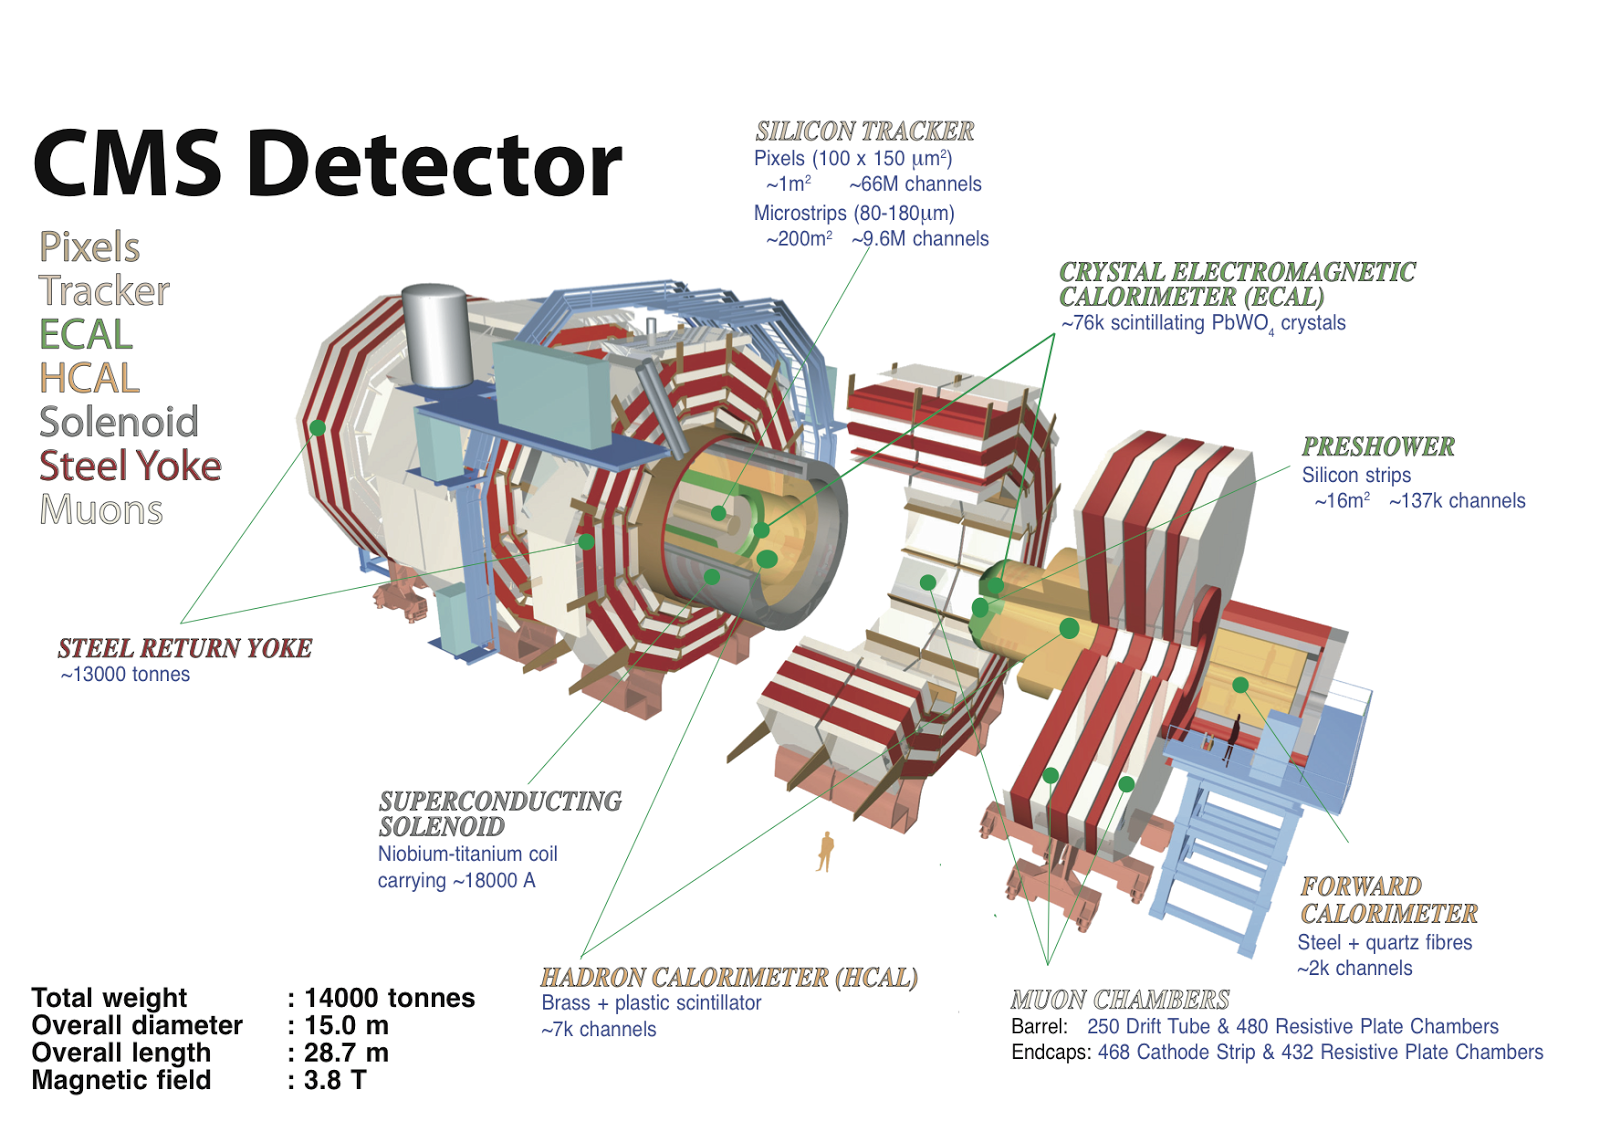
\includegraphics[width=0.9\textwidth]{figure/CH2/CMS.png}
  \end{center}
  \caption{\label{fig:CMS}Structure overview of the CMS detector.}
\end{figure}
\subsection*{Coordinate System}

The CMS coordinate system is oriented such that the $x$-axis points to the center of the LHC ring, the $y$-axis points vertically upward and the $z$-axis is in the direction of the beam. The azimuthal angle $\phi$ is measured from the $x$-axis in the $xy$ plane and the radial coordinate in this plane is denoted by $r$. The polar angle $\theta$ is defined in the $rz$ plane, while the pseudo-rapidity $\eta=-ln\tan{(\theta/2)}$. The momentum component transverse to the beam direction, denoted by $p_{T}$, is computed from the $x$- and $y$-components, and the transverse energy is defined as $E_{T}=E\sin\theta$.

\subsection{Tracker}
Tracker is the most inner part of CMS that contacts the productions of collisions in the first place. It traces the charged particles' trajectories without considering their energy as possible. Physicists can reconstruct the vertices of the interaction and the momentum of charged particles by linking tracks to the collider's pipe and measuring the curves of particles under magnetic field.

The tracking system is composed of two kinds of detector, the pixel detector and silicon strip detector. The pixel detector is built from three barrel layers at $r$=44, 73, 102 mm, and two endcap disks on each side at $z$=$\pm$345, $\pm$465 mm.
\begin{figure}[hbtp]
  \begin{center}
    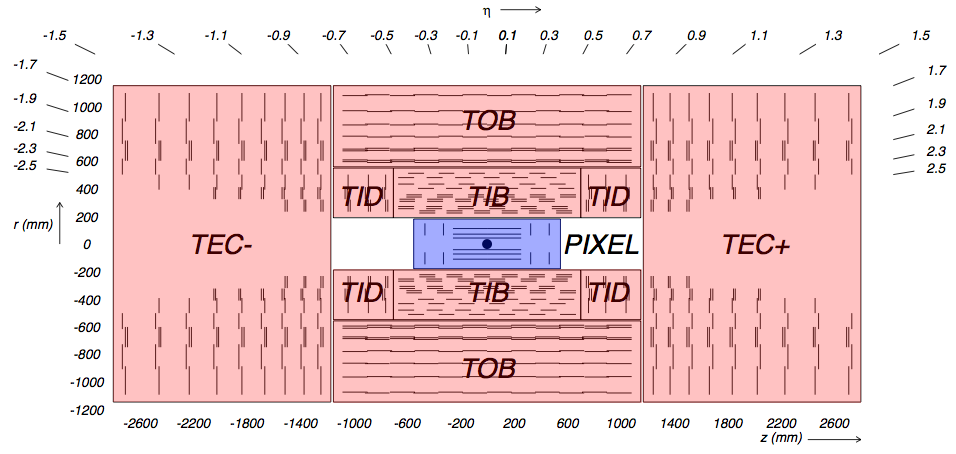
\includegraphics[width=0.9\textwidth]{figure/CH2/tracker.png}
  \end{center}
  \caption{\label{fig:tracker}Schematic layout of tracker.}
\end{figure}
\begin{figure}[hbtp]
  \begin{center}
    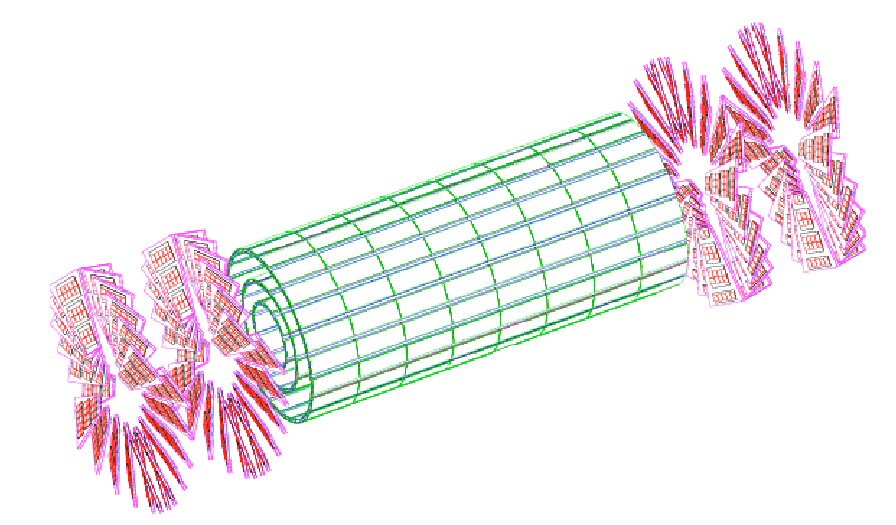
\includegraphics[width=0.4\textwidth]{figure/CH2/pixel.png}
  \end{center}
  \caption{\label{fig:pixel}The pixel detector inside tracker.}
\end{figure}
\newline And the pixel detector consists of 1440 segmented silicon sensor modules with total 66 millon readout channels. Charge carriers are distributed over several pixels. The analog pulse height information can be used to calculate the center of certain charge distribution which could improve the hit information. The spatial resolution is measured to be about 10 $\mu m$ for the $r-\phi$ plane or about 20 $\mu m$ for $z$ direction measurement.

Outside the pixel detector, there comes the silicon strip detector. The barrel region of silicon strip detector is divided into two parts, the Tracker Inner Barrel (TIB) and the Tracker Outer Barrel (TOB). The former is composed of four layers of silicon sensors with a thickness of 320 $\mu m$ and of strip pitches varying from 80 to 120 $\mu m$. The TOB is made of six layers. In this sub-detector thicker silicon sensors (500 $\mu m$) are employed, while the strip pitch varies from 120 to 180 $\mu m$. The endcap region ($|\eta| >$ 1.6) is covered by the Tracker Inner Disks (TID) and the Tracker End Cap (TEC). The entire silicon strip detector is comprised of 15200 high-sensitivity modules consisting of detecting unit, supporting structure and readout electonic system.

\subsection{ECAL}

The Electromagnetic Calorimeter (ECAL) measures the energy of photons, electrons and positrons. It it is placed just outside the tracker, but still inside the solenoid. ECAL is made of 74848 lead-tungstate (PbWO$_{4}$) crystals. This material is characterized by a high density (8.28 g/cm$^3$ ), which gives the crystals a very compact form and makes them particularly suitable to be placed inside the magnetic coil. Another reason, this material has also a fast temporal response ($\sim$10 ns) and its radiation length (X$_{0}$) of 0.89 cm give ECAL the possibility to fully contain the expansion of the electromagnetic shower.

The arrangement of ECAL is shown in Fig.~(\ref{fig:ECAL}). The barrel crystals have a front face area of 2.2 $\times$ 2.2 cm$^2$ and a length of 23 cm. They are positioned at $r$= 1.29 m in pseudo-rapidity region 0 $< |\eta| <$ 1.479. The crystals in the endcaps have a 2.47 $\times$ 2.47 cm$^2$ front face, a 22 cm length and they are positioned at $z$= 3.17 m in 1.479 $< |\eta| <$ 3.0. A Preshower detector is placed in front of the endcaps crystals. The active elements of Preshower are two planes of silicon strips with a pitch of 1.9 mm, which lie behind disks of lead absorber at depths of 2X$_{0}$ and 3X$_{0}$. It allows the rejection of photon pairs from $\pi^{0}$ decays and improvesthe estimation of the direction of photons, to enhance the measurement of the two-photon invariant mass.

The energy resolution of the ECAL is given by three different contributions\cite{EcalReso},
\begin{align}
\frac{\sigma_{E}}{E}=\frac{a}{\sqrt{E}}\oplus\frac{b}{E}\oplus c
\end{align}
where the first term is statistical in nature, it also contains fluctuation in showering and in the amplification through photodiodes (a$\sim$2.8\%), the second one considers electronic noise and pile-up (b$\sim$12\%) and the last term is mainly due to the calibration (c$\sim$0.3\%).

\begin{figure}[hbtp]
  \begin{center}
    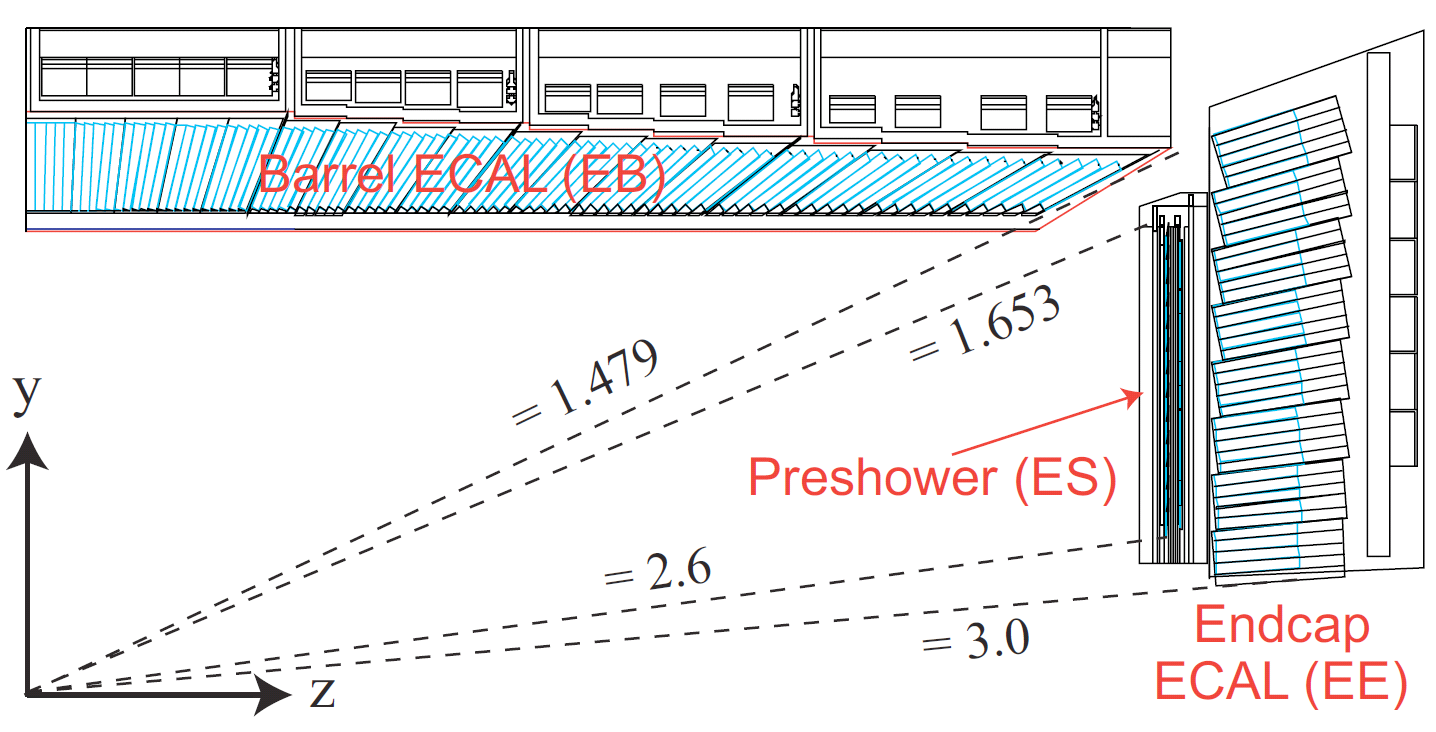
\includegraphics[width=0.9\textwidth]{figure/CH2/ECAL.png}
  \end{center}
  \caption{\label{fig:ECAL}Schematic layout of the CMS ECAL.}
\end{figure}










\subsection{HCAL}
\subsection{Muon Chamber}
\subsection{Trigger System}

% This chapter includes
% 3. Analysis procedures
%    3.1 Data sets and MC samples
%        3.1.X sub-sections for samples
%    3.2 Trigger
%    3.3 Physics objects reconstruction and identification
%        3.3.X sub-sections for physics objects

\chapter{Analysis Procedures}

In this chapter, the analysis procedures of the search for $Z'$ decaying into $Z$h in $llbb$ final state are reported. The data sets and Monte Carlo (MC) samples we used in this analysis will be indicated. Physics objects reconstruction and event selections are also introduced. Moreover, background yields and the effects of systematic uncertainties will be demonstrated in the end of this chapter.

\section{Monte Carlo Samples and Data sets}

\subsection{Signal MC}
As introduced in section 1.2.3, the signal hypothesis is HVT model B benchmark. The heavy resonance ($Z'$) is tested using a wide set of masses from 800 GeV to 2000 GeV, one masspoint every 100 GeV (Table~\ref{tab:TableSignalMC}). The signal is simulated by MadGraph5\_aMC$@$NLO\cite{MG5} in LO mode, as a narrow spin-1 neutral resonance and is forced to decay in the $Z'\rightarrow Zh\rightarrow llqq$ channel. Showering and hadronization are performed with PYTHIA6\cite{PYTHIA}.
\begin{figure}[hbtp]
  \begin{center}
    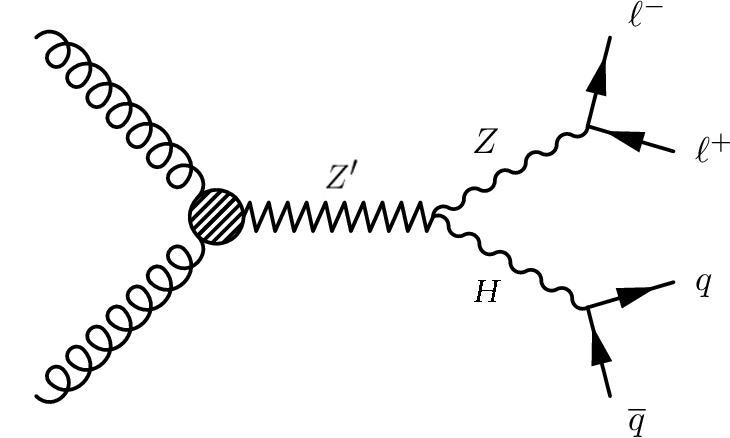
\includegraphics[width=0.4\textwidth]{figure/CH3/ZPrimeTo2l2q.png}
  \end{center}
  \caption{\label{fig:ZPrime2l2q}Feynman diagram for $Z'\rightarrow Zh \rightarrow 2l2q.$}
\end{figure}
\begin{center}
  \begin{table}
    \begin{center}
      \begin{tabular}{|c|c|c|}
        \hline
        Sample & Number of Processed Events & $\sigma_{LO}$(pb) \\ \hline
        ZPrime\_ZH\_lljj\_M800-MADGRAPH & 10710 & 0.00685367 \\ \hline
        ZPrime\_ZH\_lljj\_M900-MADGRAPH & 10209 & 0.00485861 \\ \hline
        ZPrime\_ZH\_lljj\_M1000-MADGRAPH & 19997 & 0.003263 \\ \hline
        ZPrime\_ZH\_lljj\_M1100-MADGRAPH & 9370 & 0.00217483 \\ \hline
        ZPrime\_ZH\_lljj\_M1200-MADGRAPH & 10710 & 0.00145484 \\ \hline
        ZPrime\_ZH\_lljj\_M1300-MADGRAPH & 9369 & 0.000979745 \\ \hline
        ZPrime\_ZH\_lljj\_M1400-MADGRAPH & 10497 & 0.000664783 \\ \hline
        ZPrime\_ZH\_lljj\_M1500-MADGRAPH & 19999 & 0.000454339 \\ \hline
        ZPrime\_ZH\_lljj\_M1600-MADGRAPH & 8950 & 0.000312541 \\ \hline
        ZPrime\_ZH\_lljj\_M1700-MADGRAPH & 9369 & 0.000216282 \\ \hline
        ZPrime\_ZH\_lljj\_M1800-MADGRAPH & 10708 & 0.000150398 \\ \hline
        ZPrime\_ZH\_lljj\_M1900-MADGRAPH & 10498 & 0.000105039 \\ \hline
        ZPrime\_ZH\_lljj\_M2000-MADGRAPH & 19999 & 7.36377e-05 \\
        \hline
      \end{tabular}
    \end{center}
    \caption{\label{tab:TableSignalMC}Signal samples used in the analysis.}    
  \end{table}
\end{center}
\newpage
\subsection{Background MC}
Since we are looking for new resonances decaying in semi-leptonic final state, the background samples of this analysis are originated by all SM events with two leptons and at least one jet as final state. The dominant background contribution is the produciton of Z boson with jets. This Z+jets sample is produced by MADGRAPH. In the matrix element level, the Z boson is forced decaying into two leptons, and further this sample is divided into two samples depending on the Z $p_{T}$, higher than 100 GeV or between 70 and 100 GeV. The contribution of events with Z $p_{T}$ less than 70 GeV is negligible due to further cut on the objects $p_{T}$ in the selection criteria.

The second dominant source of background is $t\bar{t}$ production. Both of the two top quarks decay into all leptonic final state (top decays into a W boson and a b quark first) which gives two leptons, neutrinos and two b-jets. This sample is generated by POWHEG\cite{POWHEG}.

Other sources of background considered are SM di-boson productions (WW, WZ and ZZ) generated by PYTHIA6. All the background samples are required to pass phase-space cuts, $p_{T}^{ll} > $60 GeV and 60$ < M_{ll} < $120 GeV. Related statistics are reported in Table~\ref{tab:TabBkgMC}.

\begin{center}
  \begin{table}[h]
    \begin{center}
      \begin{tabular}{|c|c|c|}
        \hline
        Sample & Number of Processed Events & $\sigma_{NLO}$(pb) \\ \hline
        DYJetsToLL\_PtZ-70To100 & 11764538 & 63.5 \\ \hline
        DYJetsToLL\_PtZ-100 & 12511326 & 39.4 \\ \hline
        TTTo2L2Nu2B & 10783509 & 25.8 \\ \hline
        WW & 7759752 & 56.0 $\pm$ 2.3 ($\pm$ 0.3) \\ \hline
        WZ & 9910267 & 22.4 \\ \hline
        ZZ & 9769891 & 7.6 $\pm$ 0.3 ($\pm$ 0.3)\\
        \hline
      \end{tabular}
    \end{center}
    \caption{\label{tab:TabBkgMC}Background samples used in the analysis.}    
  \end{table}
\end{center}

\subsection{Data Samples}
In this analysis, the full CMS data collected in 2012 is used, corresponding to the integrated luminosity of 19.7 fb$^{-1}$ at center-of-mass energy $\sqrt{s} = $8 TeV. For each lepton channel, there are four datasets. All datasets are collected with a double muon or a double electron trigger, as explained in detail in the next section. The trigger algorithm employed for the electron samples doesn't use any information from the tracker but only the energy deposite in the ECAL. This expedient is implemented in order to avoid any possible inefficiencies due to the presence of two tracks very close to each other when the Z is highly boosted and its decay products are very collimated. Such a trigger is contained in the Photon/DoublePhotonHighPt dataset. The full dataset names are listed in Table~\ref{tab:TabDataSet}.

\begin{center}
  \begin{table}[h]
    \begin{center}
      \begin{tabular}{|c|c|}
        \hline
        AOD Sample & Luminosity (pb$^{-1}$) \\ \hline
        DoubleMu/Run2012A-22Jan2013-v1 & 876.225 \\ \hline
        DoubleMuParked/Run2012B-22Jan2013-v1 & 4409 \\ \hline
        DoubleMuParked/Run2012C-22Jan2013-v1 & 7017 \\ \hline
        DoubleMuParked/Run2012D-22Jan2013-v1 & 7369 \\ \hline
        Photon/Run2012A-22Jan2013-v1 &  876.225 \\ \hline
        DoublePhotonHighPt/Run2012B-22Jan2013-v1 & 4412 \\ \hline
        DoublePhotonHighPt/Run2012C-22Jan2013-v1 & 7055 \\ \hline
        DoublePhotonHighPt/Run2012D-22Jan2013-v1 & 7369 \\
        \hline
      \end{tabular}
    \end{center}
    \caption{\label{tab:TabDataSet}Data sets used in this analysis.}    
  \end{table}
\end{center}

\section{Trigger}
Since the final state contains two same flavour leptons and at least one jet, we perform this analysis on the DoubleMu and Photon/DoublePhotonHighPt datasets. The first dataset is triggered by two muons, the second one is triggered by two eletrons. These triggers are:
\begin{itemize}
\item HLT\_Mu22\_TkMu8* (for DoubleMu datasets)
\item HLT\_DoubleEle33\_* (for Photon/DoublePhontonHighPt datasets)
\end{itemize}

The muon trigger has a double $p_{T}$ threshold, requires leading muon $p_{T}$ greater than 22 GeV and sub-leading muon $p_{T}$ greater than 8 GeV. Differently, the double electron trigger requires a higher threshold of 33 GeV to electrons. The trigger efficiencies are close to 1 in both cases.

\section{Physics Objects}

\subsection{Muon}
\subsection*{Reconstruction}
The muon reconstruction algorithm at CMS takes advantage of the redundancy of detection methods. Muon tracks are first reconstructed independently in the inner tracker (tracker track) and in the muon system (standalone track). Based on these objects, two reconstruction approaches are used\cite{MuonReco}:
\begin{itemize}
\item $Globol~Muon$ (outside-in): Starting from a standalone track, this algorithm finds a best tracker track to match the standalone track. Then, the fit of the track is repeated using the hits both in the tracker and in the muon system\cite{KF}. The resulting object is called a $Global~Muon$. At large transverse momentum ($p_{t} > $200 GeV), the global muon fit can improve the momentum resolution compared to the tracker only fit.
\item $Tracker~Muon$ (inside-out): A tracker muon is reconstructed by an opposite direction from a global muon. In this approach, all tracker tracks with $p_{T} >$ 0.5 GeV and the total momentum $p >$ 2.5 GeV are considered as possible muon candidates. The extrapolation to the muon system takes into account the magnetic field, average expected energy losses, and multiple scattering in the detector material. If at least one muon segment matches the extrapolated track, the corresponding track track qualifies as a $Tracker~Muon$. This algorithm is useful for low-$p_{T}$ muons that are not fully penetrate the muon system, and therefore only register a few hits
\end{itemize}

If no match is found when extrapolating outside-in, the standalone track is stored as a $Stanalone~Muon$. This happens only for less than 1\% of the muons produced in a collison, and the reconstruction efficiency is about 99\% for the muon which carries enough high momentum within detector coverage\cite{MuonReco}.

\newpage
\subsection*{Identification}
We use both tracker muons and global muons in this analysis. To identify muons from the signal, the muons must pass one of these two off-line selections, high$-p_{T}$ muon ID or tracker-based muon ID\cite{MuonID}. The requirements are listed as follows:\\

High-$p_{T}$ muon ID
\begin{itemize}
\item Muon identified as a $Global~Muon$.
\item Number of muon hits in the global track $> 0$.
\item Number of matched muon stations $> 1$.
\item Number of pixel hits $> 0$.
\item Number of tracker layer with hits $> 8$.
\item Transverse impact parameter $d_{xy} < 0.2$ cm.
\item Longitudinal impact parameter $d_{z} < 0.5$ cm.
\item Relative error on the track transverse momentum $\sigma_{p_{T}}/p_{T} < 0.3$.\\
\end{itemize}

In the tracker-based muon ID, the muon has to be identified as a $Tracker~Muon$, and the requirement of muon hits in the global track is removed. Other requirements are the same.

An additional useful variable for lepton identification is the isolation. It is defined as the scalar sum of the $p_{T}$ of the reconstructed objects within a cone (typical size is $\Delta R=0.3$) space around the lepton track but excluding the $p_{T}$ of the lepton itself. Moreover, the relative isolation is defined as isolation divided by the lepton $p_{T}$ ($I_{rel} = Iso/p_{T}^{lep}$). The relative isolation is more frequently used in the modern analysis.

In this analysis, a modified isolation criteria is used. The two muons originated from boosted Z decay are close to each other, and consequently the presence of another muon in the isolation cone could break the function of this variable. To solve this problem, we exclude the energy contribution of muons inside the cone.

\begin{align}
  \label{eq:ModIso}
  I_{rel}^{mod}=\frac{\sum p_{T}^{CH}+max(0.0 , \sum E_{T}^{NH}+\sum E_{T}^{\gamma}-0.5\times \sum p_{T}^{PU})}{p_{T}^{lep}}
\end{align}

In the above equation, $p_{T}^{CH}$ denotes the charged hadron transverse momentum inside the cone. Similarly, $E_{T}^{NH}$ and $E_{T}^{\gamma}$ stand for neutral hadron and photon transverse energy respectively. The last term in the nomimator, $\sum p_{T}^{PU}$ is defined as sum of transverse momentum of the charged particles in the cone but with particles not originating from the primary vertex (for pile-up corrections). Finally, the modified requirement is $I_{rel}^{mod} < 0.1$.\\

\begin{table}[h]
  \begin{center}
    \begin{tabular}{|l|c|c|}
      \hline
      Variable & Standard & Modified \\ \hline
      Muon type & Global muon & Tracker muon \\
      Muon hits in global track & $\geq$ 1 & - \\
      Muon stations matched & $\geq$ 2 & $\geq$ 2 \\
      $d_{xy}$ & $<$ 0.2 cm & $<$ 0.2 cm\\
      $d_{z}$ & $<$ 0.5 cm & $<$ 0.5 cm\\
      Pixel hits & $\geq$ 1 & $\geq$ 1 \\
      Tracker layers & $\geq$ 8 & $\geq$ 8 \\
      $\sigma_{p_{T}}/p_{T}$ & $<$ 0.3 & $<$ 0.3 \\ \hline
      $I_{rel}^{mod}$  & $<$ 0.1 & $<$ 0.1 \\
      \hline
    \end{tabular}
    \caption{\label{tab:MuonIDtable} Summary of the muon ID selection criteria.}
  \end{center}
\end{table}


\subsection{Electron}
\subsection*{Reconstruction}
Text.

%% This textfile includes
% 3. Analysis procedures
%    ..
%    ..
%    ..
%    3.3 Event and Object selection
%    3.4 Data and MC comparison
%    3.5 Background estimation
%
\section{Pile-up reweighting}
At the typical luminosity provided by the LHC, it is common to reconstruct more than one vertex per event. The main event vertex is defined as the one with the highest sum of the $p_{T}^{2}$ of the associated tracks. The presence of additional interactions, known as pile-up (PU). 

The simulation generates the pile-up roughly to match the condiction in data, however there are still difference between the pile-up numbers in data and MC. It is neccesary to reweight pile-up distribtuions of MC samples to match the data more precisely. By applying a proper weight to each MC event according to the pile-up distribution from data, the MC samples can describe the data better. Fig.~\ref{fig:PUreweight} shows the number of vertices after pile-up reweighting in both two lepton channel.

\begin{figure}[hbtp]
  \centering
  \subfigure[Number of vertices in muon channel]{
    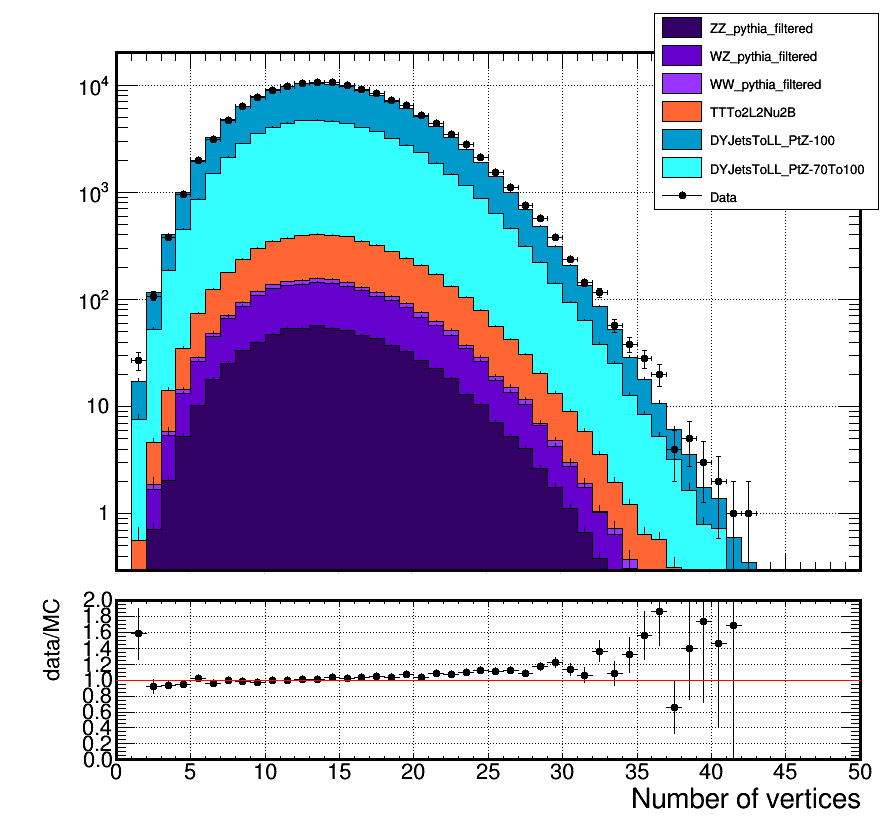
\includegraphics[scale=0.22]{figure/CH3/h_nVtx_Mu.png}}
  \hspace{0.5cm}
  \subfigure[Number of vertices in electron channel]{
    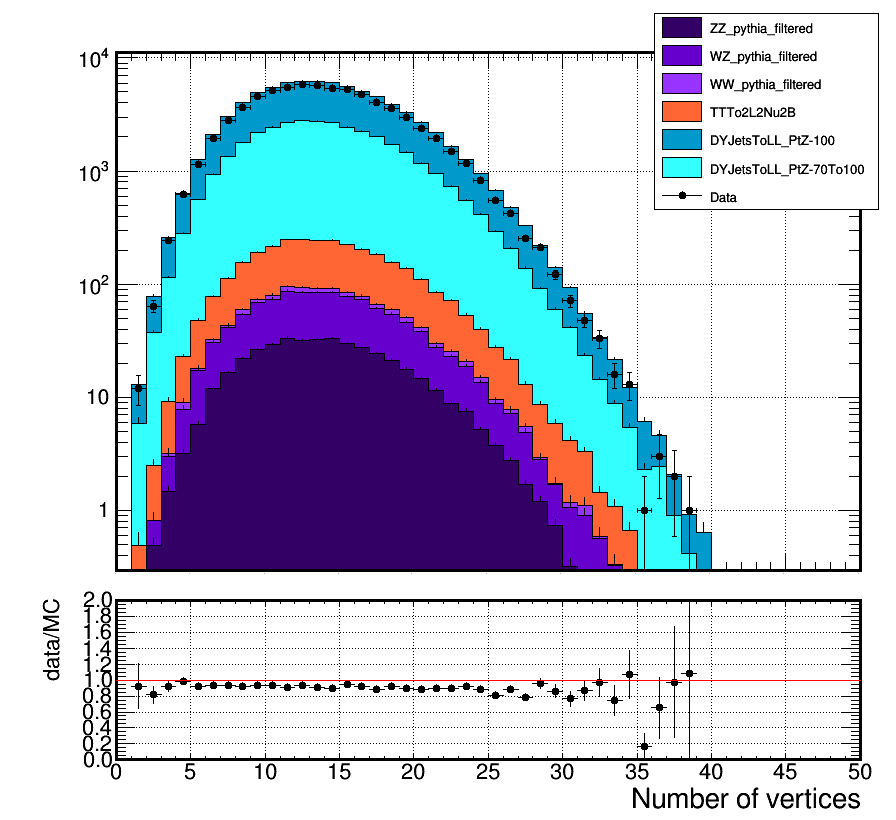
\includegraphics[scale=0.22]{figure/CH3/h_nVtx_El.png}}
  \caption{\label{fig:PUreweight}Number of vertices distributions after pile-up reweighting. Data are compared to the combination of all MC background samples. After reweighting, the distributions are almost identical to the data in both channels.}
\end{figure}



\newpage
\section{Event and Object selection}


\subsection{Lepton Requirements}

\subsection*{Muon Selection}

Besides the muon ID criteria disscussed in section 3.3.1 (Table~\ref{tab:MuonIDtable}), we also require kinematic cuts on the muon candidates. We select the transverse momentum of the leading muon candidate must greater than 40 GeV, while the second leading muon transverse momentum threshold is 20 GeV. All muon candidates are must in the psuedo-rapidity $|\eta| < 2.4$ region.

\subsection*{Electron Selection}
Kinematic cuts on the electron candidates are also applied. Although the electron ID selection (Table~\ref{tab:EleIDtable}) already required the pseudo-rapidity of electron supercluster, we cut on the $|\eta| < 2.5$ for electron candidates and all electrons must out of [1.4442,1.566] in the $\eta$ region to avoid the ECAL gap. The $p_{T}$ requirement is a bit different from the muon case. Since the HLT trigger already selects electron $p_{T}$ greater than 33 GeV, we require both leading and sub-leading electrons $p_{T}$ greater than 40 GeV in advance.

\subsection{Jet Requirement}
CA8jets in our signal process is originated from Higgs decay. If the $Z'$ mass is large enough, the Higgs will be boosted. Therefore we require higher kinematic thresholds to the CA8jets. In every event, there must find at least one CA8jet with $p_{T} > 80$ GeV, $|\eta| < 2.4$, passing loose jet ID and the pruned-jet mass must greater than 40 GeV to remove jets from backgrounds.

Futhermore, in order to veto leptons that are mis-identified as jets, leptons overlap with jets are removed by the $\Delta R$ cut, i.e. if there's a lepton passing all lepton selections and the spatial distance to a CA8jet smaller than 0.1 ($\Delta R_{jet,lepton} < 0.1$), then the jet will be removed.

\subsection{Z boson Requirement}
The Z boson candidate is reconstructed by adding four-momentum of the selected lepton pair. Since the Z boson mass is about 91 GeV, we require the reconstructed invariant mass of the Z boson in the mass region [70 GeV, 110 GeV] where is $\pm 20$ GeV to its theoretical mass.

For the CA8jet from Higgs, we require $p_{T}$ threshold as 80 GeV. The kinematics of reconstructed Z boson and Higgs should be symmetric, because they are both decayed from the heavy $Z'$, comparing their mass to $Z'$, the difference between 125 GeV and 91 GeV is negligible ($1\textup{ TeV} >> 125 \textup{ GeV} \sim 91 \textup{ GeV}$). Therefore we require the same $p_{T}$ theshold to the Z boson. Fig.~\ref{fig:genZHPt} shows the transverse momentum distributions from the signal samples.

\begin{figure}[hbtp]
  \centering
  \subfigure[generator level Higgs $p_{T}$ distribustion]{
    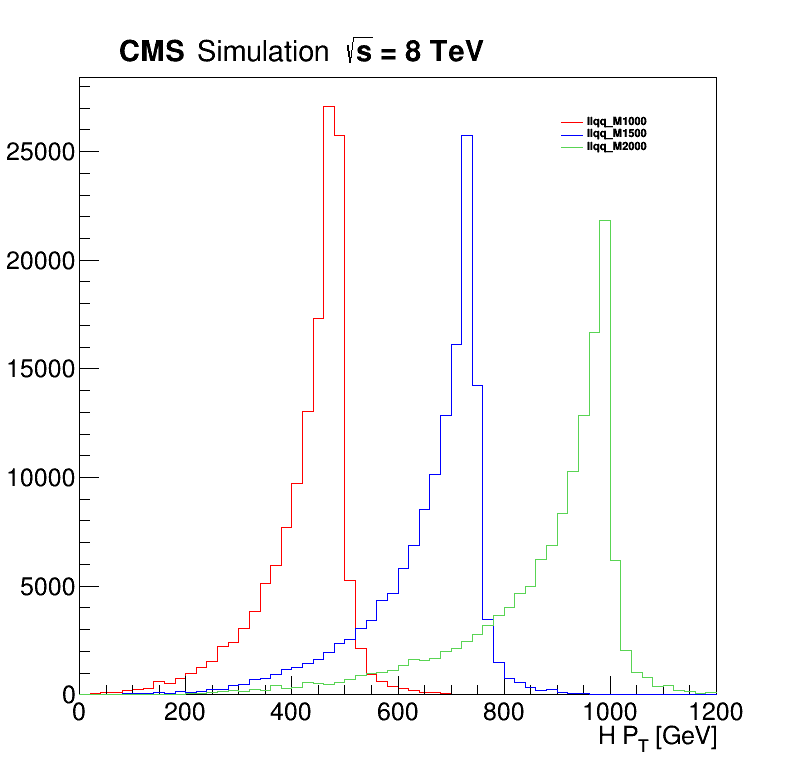
\includegraphics[scale=0.25]{figure/CH3/h_genHPt.png}}
  \hspace{0.5cm}
  \subfigure[generator level Z boson $p_{T}$ distribustion]{
    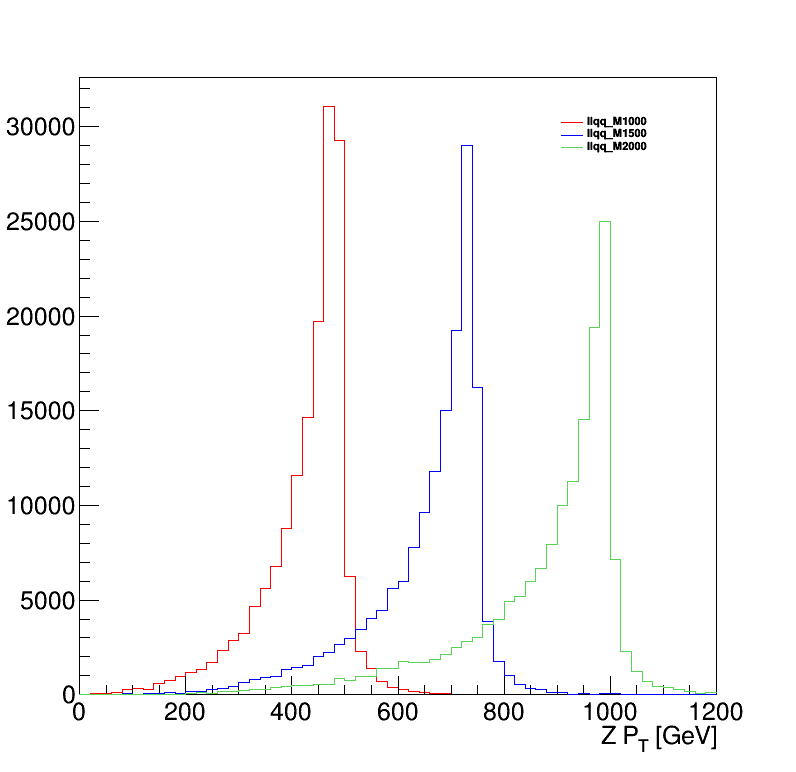
\includegraphics[scale=0.25]{figure/CH3/h_genZPt.png}}
  \caption{\label{fig:genZHPt}Z and Higgs $p_{T}$ distribution are almost identical. We pick three samples with different mass points of $Z'$, 1000 GeV (red), 1500 GeV (blue) and 2000 GeV (green). These plots are made from the generator level signal samples without any proper selections.}
\end{figure}

Finally, all selection requirements are summarized in Table~\ref{tab:preselection}.
\newpage

\begin{center}
  \begin{table}[h]
    \begin{center}
      \begin{tabular}{|lcc|}
        \hline
        \textbf{Selection} & \textbf{Value} & \textbf{Comments} \\ \hline
        Trigger & HLT\_Mu22\_TkMu8 & DoubleMu dataset \\
        & HLT\_DoubleEle33 & DoublePhoton dataset \\ \hline
        Leading muon $p_{T}$ & $p_{T} > 40$ GeV &\\
        Sub-leading muon $p_{T}$ & $p_{T} > 20$ GeV &\\
        Muon $\eta$ & $|\eta| < 2.4$ &\\
        Muon ID & High $p_{T}$ tracker based &\\
        Muon isolation $I_{trk}^{mod}$ & $< 0.1$ &\\ \hline
        Leading electron $p_{T}$ & $p_{T} > 40$ GeV &\\
        Sub-leading electron $p_{T}$ & $p_{T} > 40$ GeV &\\
        Electron $\eta$ & $|\eta| < 2.5$ &\\
        & out of [1.4442,1.566] & To avoid ECAL gap. \\
        Electron ID & HEEP modified &\\
        Electron isolation  & &\\
        $I_{trk}^{mod}$ & $<$ 5 GeV &\\
        $I_{ECAL,HCAL}^{mod}$ & $<$ 2 GeV + 0.03$E_{T}$ & Barrel \\
        & $< 2.5$ GeV & for $E_{T} < 50$ GeV candidates in Endcap\\
        & $< 2.5$ GeV + 0.03$E_{T}$ & for $E_{T} > 50$ GeV candidates in Endcap\\ \hline
        Jet ID & Loose working point &\\
        Jet $p_{T}$ & $p_{T} > 80$ GeV &\\
        Jet $\eta$ & $|\eta| < 2.4$ &\\
        Prunedjet mass & $> 40$ GeV &\\
        Veto jet-lepton overlap & $\Delta R_{jet,lepton} < 0.1$ & Remove the jet satisfies this requirement.\\ \hline
        Z $p_{T}$ & $p_{T} > 80$ GeV &\\
        Z mass window cut & $70 \textup{ GeV} < m_{Z} < 110 \textup{ GeV}$ &\\
        \hline
      \end{tabular}
    \end{center}
    \caption{\label{tab:preselection}Event and object selection requirements used in the analysis.}
  \end{table}
\end{center}

\newpage
\section{Data-MC comparison}

In this section, a comparison between data and simulation is reported for various kinematic observables. It can be seen that the dominant background contribution comes from the Z+jets production, while sub-leading contributions are from $t\bar{t}$ and dibosons can be negligible.

On top of the selections described in previous section, additional regions are defined as following:

\begin{itemize}
\item \textbf{Signal region (SR)}: Represents the phase space where the signal is expected, defined by the prunedjet mass in $110 \textup{ GeV} < m_{prunedjet} < 140 \textup{ GeV}$ region. The range is chosen by $\pm$15 GeV to the mass of Higgs.
\item \textbf{Sidebands (SB)}: Defined by the interval between $70 \textup{ GeV} < m_{prunedjet} < 110 \textup{ GeV}$. This region is signal-depleted. In our case, we don't consider prunedjet mass higher than 140 GeV, because of the poor statistics and the excessive contribution of $t\bar{t}$ events.
\end{itemize}

In the following plots, the data-MC comparison is performed in SB region and all background samples are weighted to the same luminosity as data. Because the signal region in data is considered \textbf{blind} in this analysis stage, so they are not shown.

\begin{figure}[hbtp]
  \centering
  \subfigure[Muon energy fraction]{
    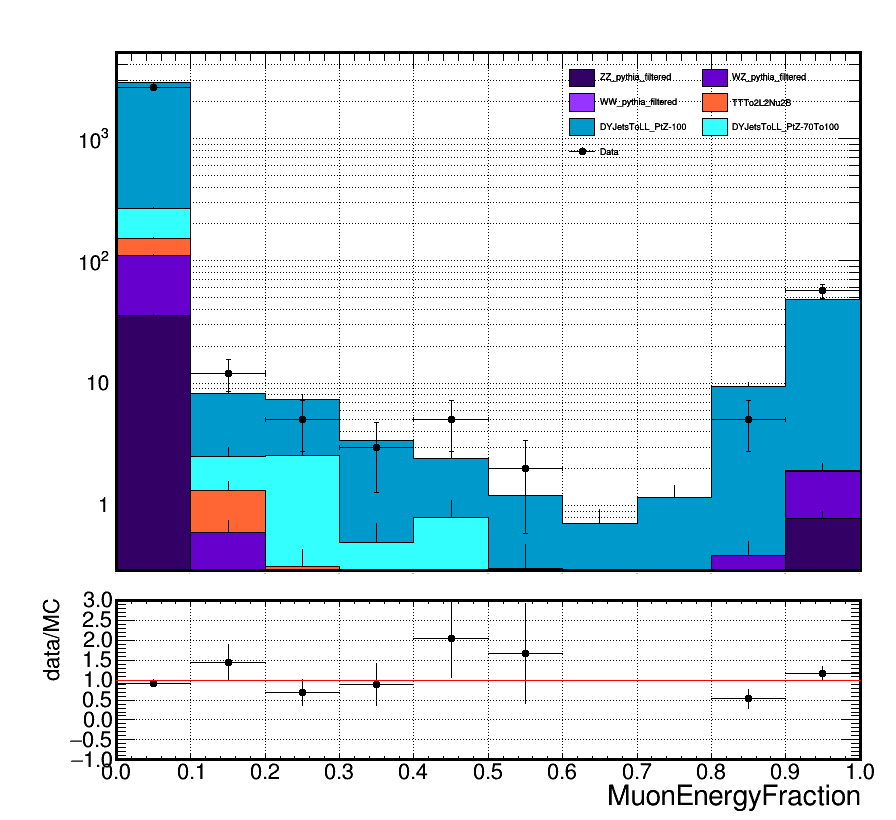
\includegraphics[scale=0.22]{figure/CH3/JetID/h_CA8jetMuEF.png}}
  \hspace{0.5cm}
  \subfigure[Photon energy fraction]{
    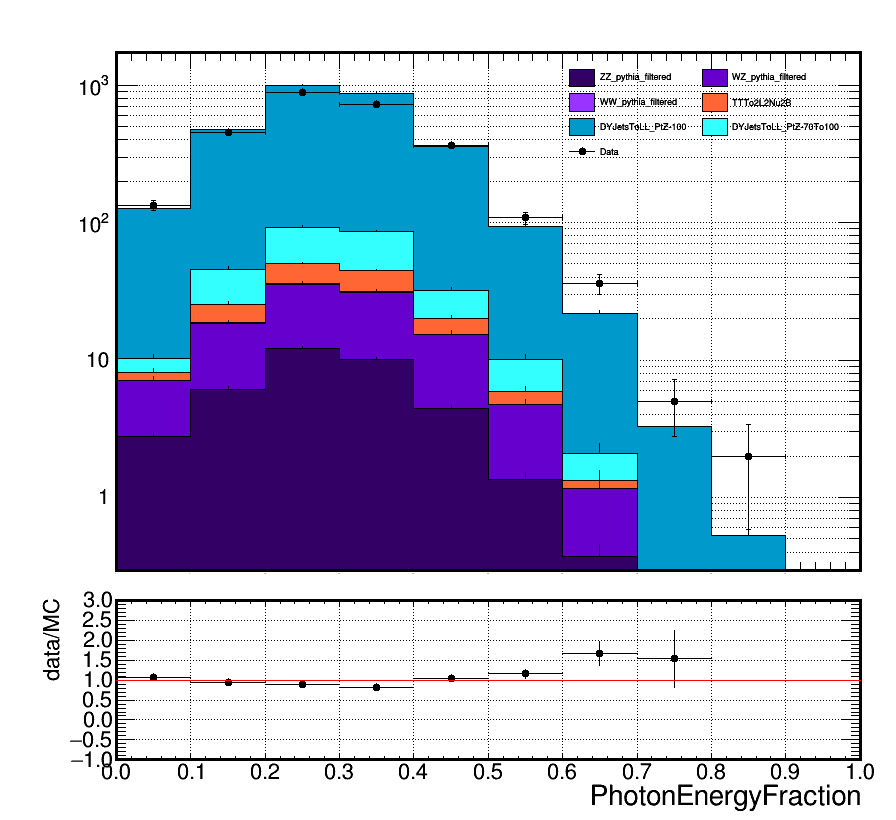
\includegraphics[scale=0.22]{figure/CH3/JetID/h_CA8jetPhoEF.png}}
  \caption{\label{fig:MuPhoEF}Comparison between data and all background samples for two jet variables. The definition of muon/photon  energy fraction is muon/photon energy divided by jet energy.}
\end{figure}

\begin{figure}[hbtp]
  \centering
  \subfigure[Charged electromagnetic energy fraction]{
    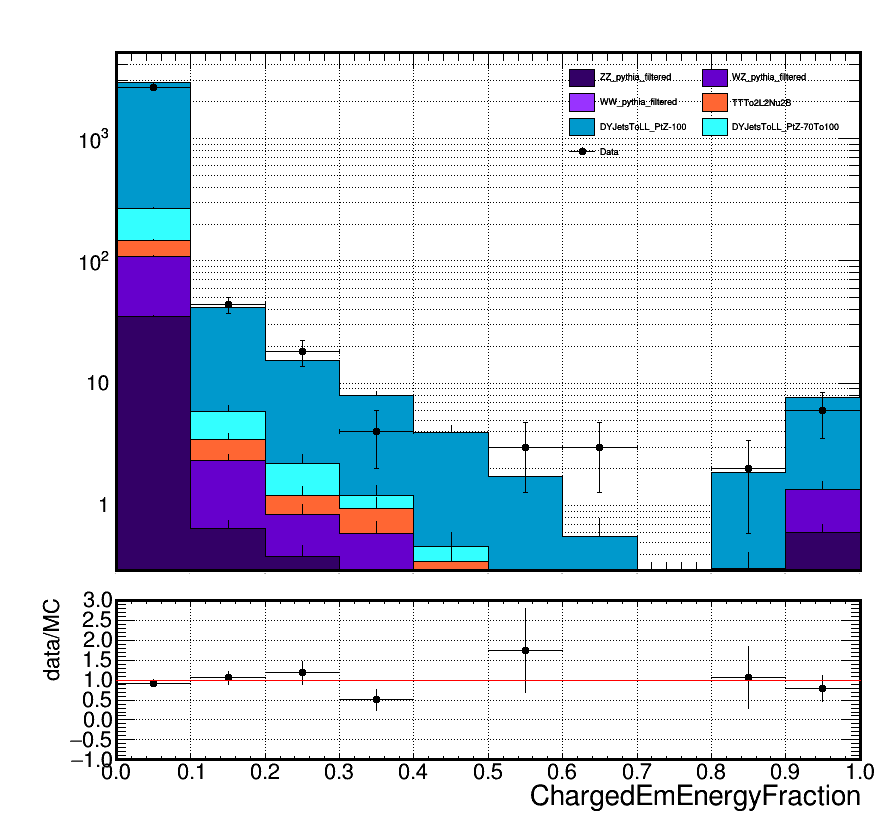
\includegraphics[scale=0.22]{figure/CH3/JetID/h_CA8jetCEmEF.png}}
  \hspace{0.5cm}
  \subfigure[Charged hadron energy fraction]{
    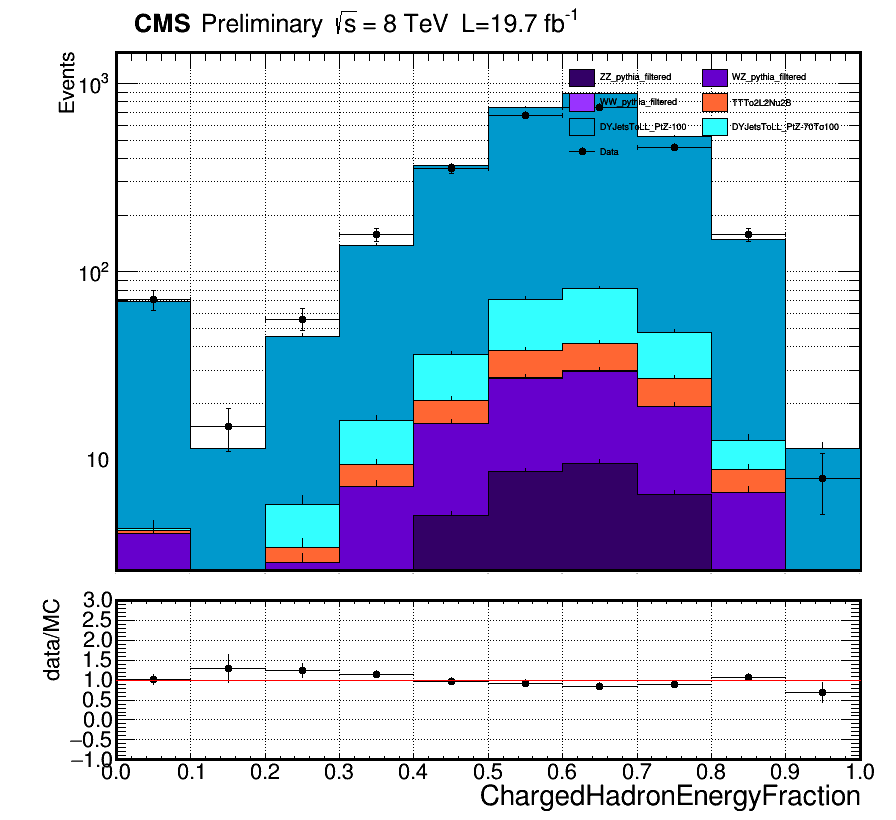
\includegraphics[scale=0.22]{figure/CH3/JetID/h_CA8jetCHadEF.png}}
  \caption{\label{fig:ChargedEF}Charged electromagnetic/hadron energy fraction is defined by the ratio of the energy of charged particles in ECAL/HCAL to the jet energy.}
\end{figure}

\begin{figure}[hbtp]
  \centering
  \subfigure[Neutral electromagnetic energy fraction]{
    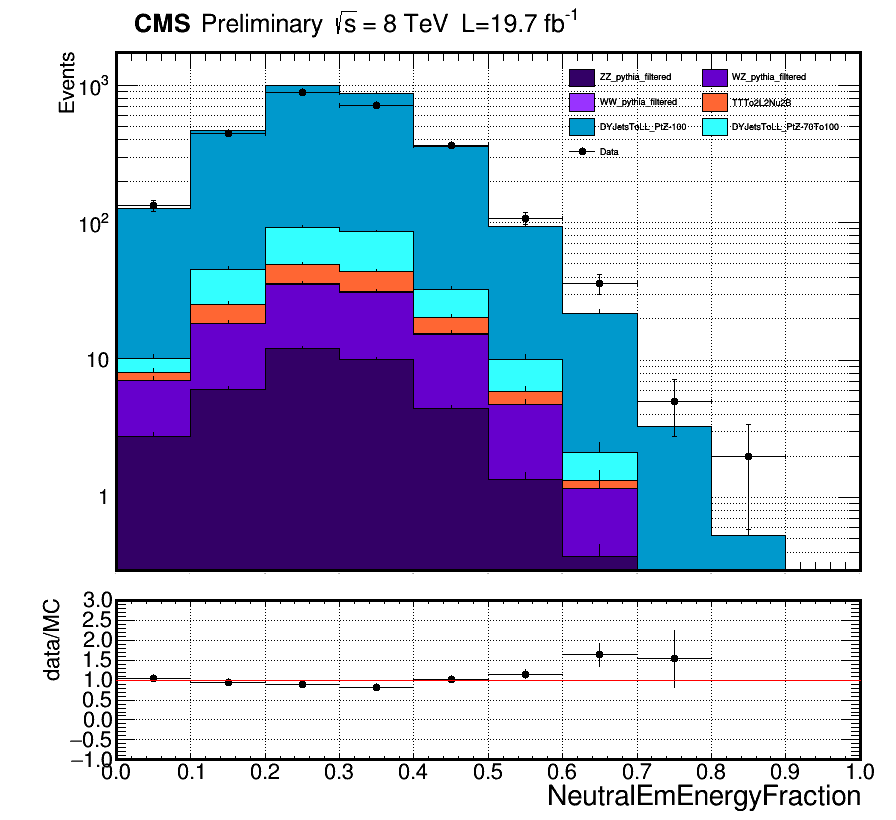
\includegraphics[scale=0.22]{figure/CH3/JetID/h_CA8jetNEmEF.png}}
  \hspace{0.5cm}
  \subfigure[Neutral hadron energy fraction]{
    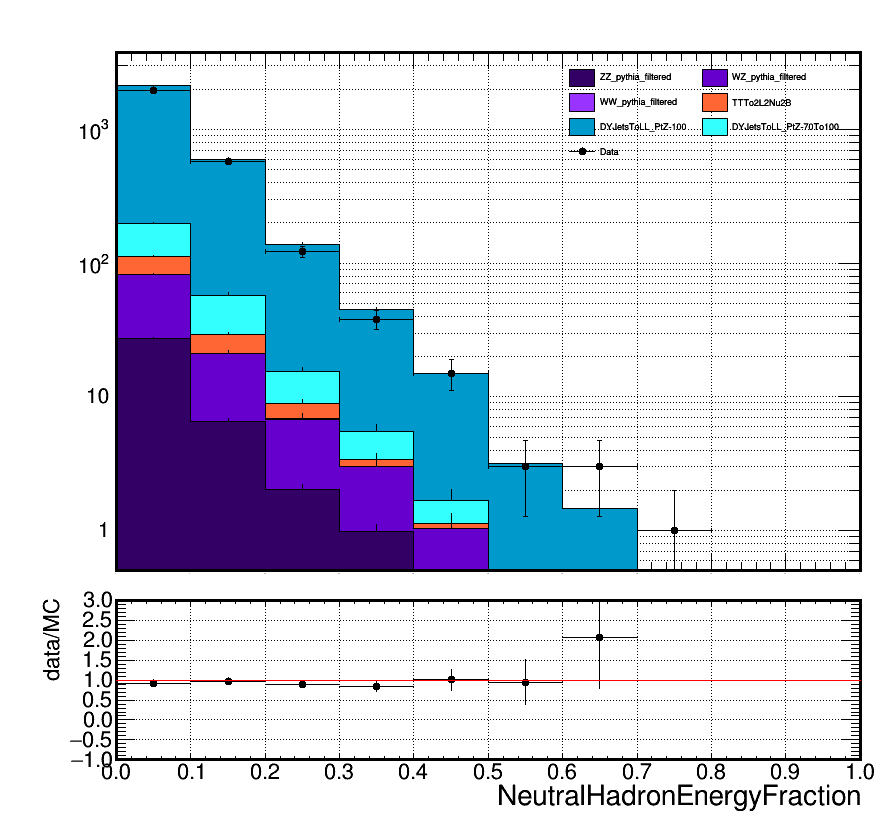
\includegraphics[scale=0.22]{figure/CH3/JetID/h_CA8jetNHadEF.png}}
  \caption{\label{fig:NeutralEF}Neutral electromagnetic/hadron energy fraction is defined by the ratio of the energy of neutral particles in ECAL/HCAL to the jet energy.}
\end{figure}

\begin{figure}[hbtp]
  \centering
  \subfigure[Jet multiplicity]{
    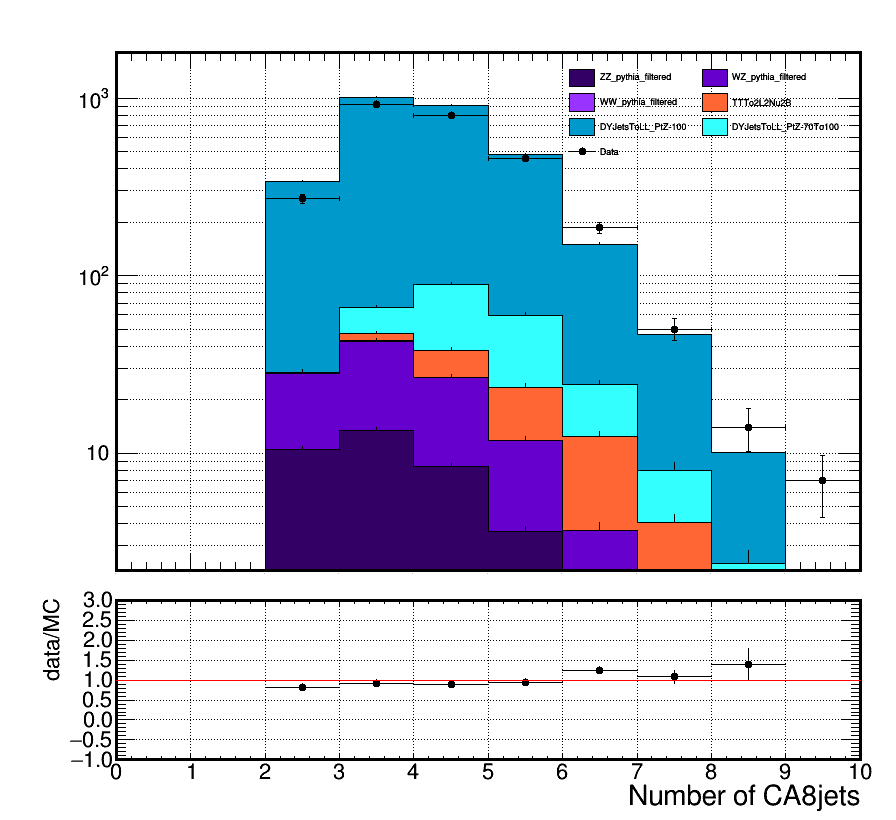
\includegraphics[scale=0.22]{figure/CH3/Jet_kinematics/h_nCA8jet.png}}
  \hspace{0.5cm}
  \subfigure[CA8jet $p_{T}$]{
    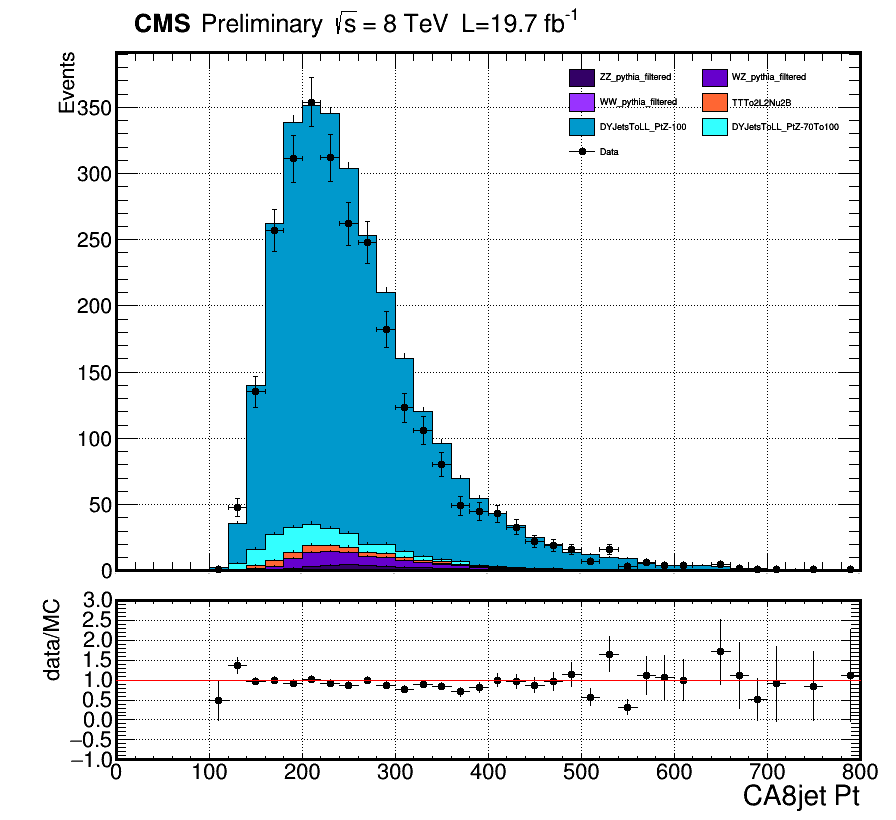
\includegraphics[scale=0.22]{figure/CH3/Jet_kinematics/h_CA8jetPt.png}}
  \caption{\label{fig:nCA8jetPt}Comparison between data and MC in SB region using jet multiplicity (number of jets) and CA8jet transverse momentum.}
\end{figure}

\begin{figure}[hbtp]
  \centering
  \subfigure[CA8jet $\eta$]{
    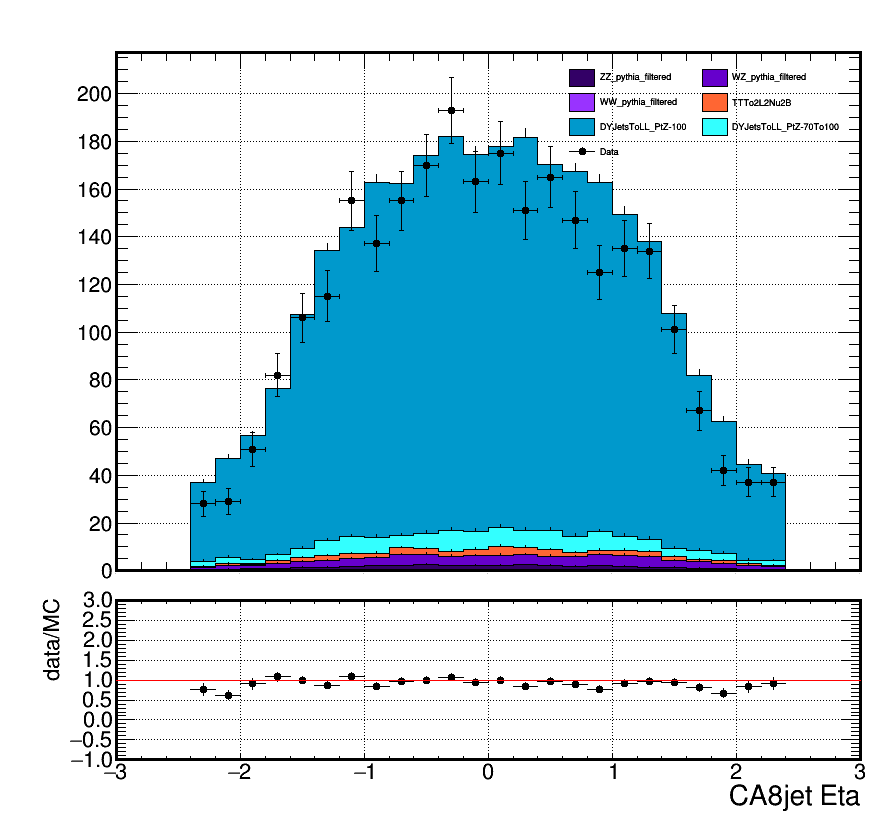
\includegraphics[scale=0.22]{figure/CH3/Jet_kinematics/h_CA8jetEta.png}}
  \hspace{0.5cm}
  \subfigure[CA8jet $\phi$]{
    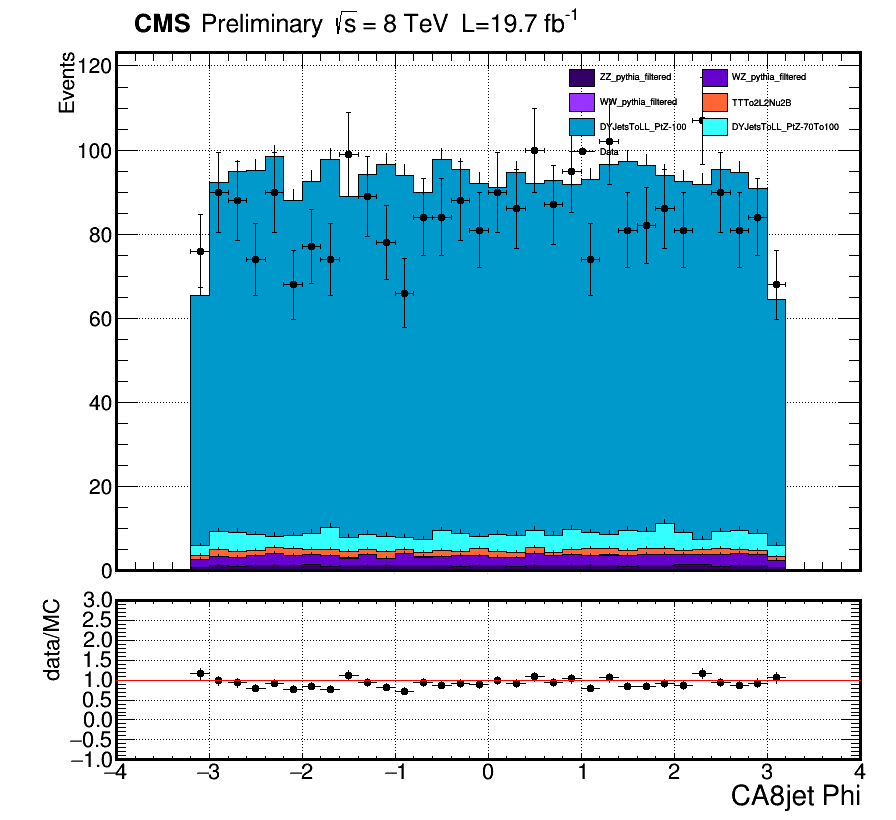
\includegraphics[scale=0.22]{figure/CH3/Jet_kinematics/h_CA8jetPhi.png}}
  \caption{\label{fig:CA8jetEtaPhi}Comparison between data and MC in SB region using CA8jet $\eta$ and $\phi$.}
\end{figure}

\begin{figure}[hbtp]
  \centering
  \subfigure[Prunedjet mass]{
    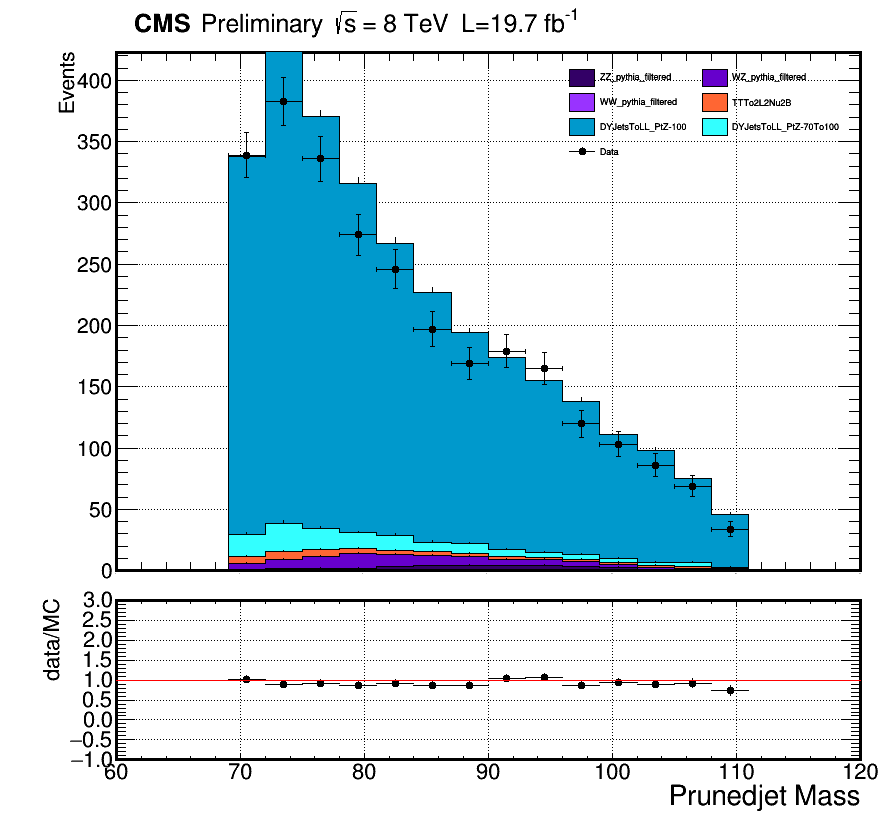
\includegraphics[scale=0.22]{figure/CH3/Jet_kinematics/h_PrunedjetM.png}}
  \hspace{0.5cm}
  \subfigure[$\Delta R$ between two subjets]{
    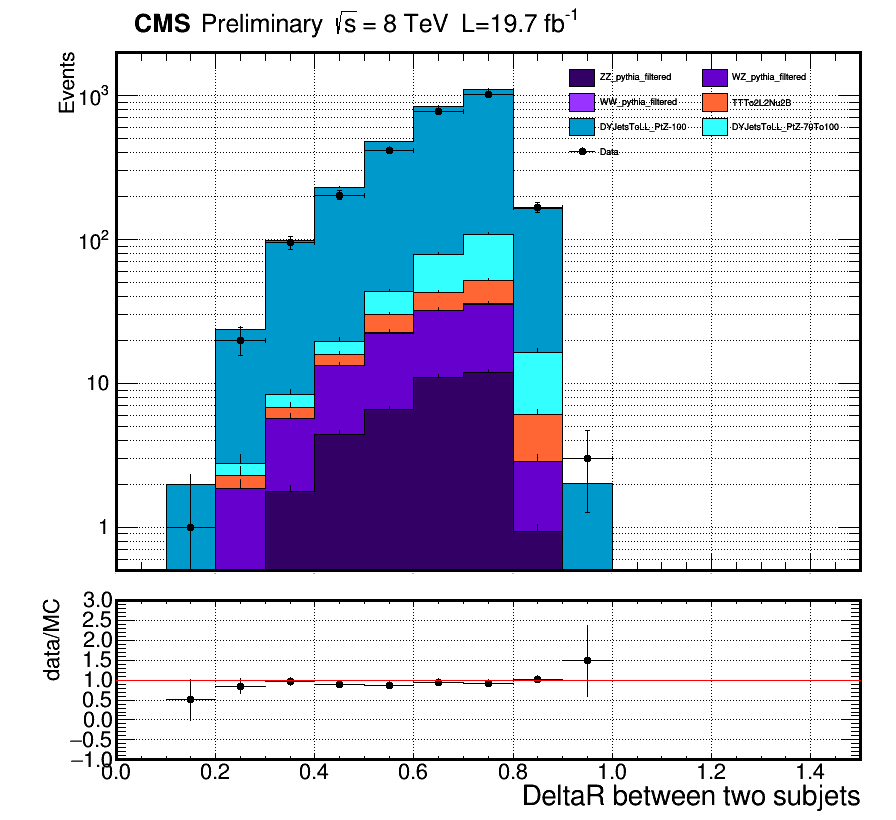
\includegraphics[scale=0.22]{figure/CH3/Jet_kinematics/h_DeltaRjj.png}}
  \caption{\label{fig:prunedmassDRjj}Left: the prunedjet mass in the SB region. Right: the spatial distance between two subjets within the CA8jet.}
\end{figure}

\begin{figure}[hbtp]
  \centering
  \subfigure[Z mass]{
    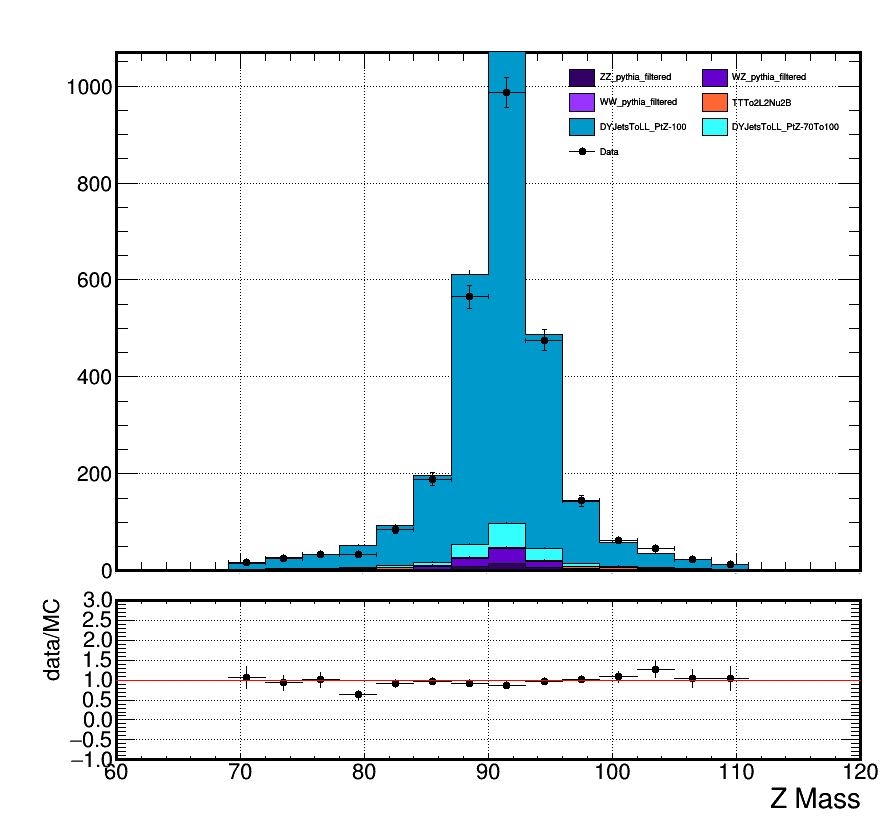
\includegraphics[scale=0.22]{figure/CH3/Z_kinematics/h_ZMass.png}}
  \hspace{0.5cm}
  \subfigure[Z $p_{T}$]{
    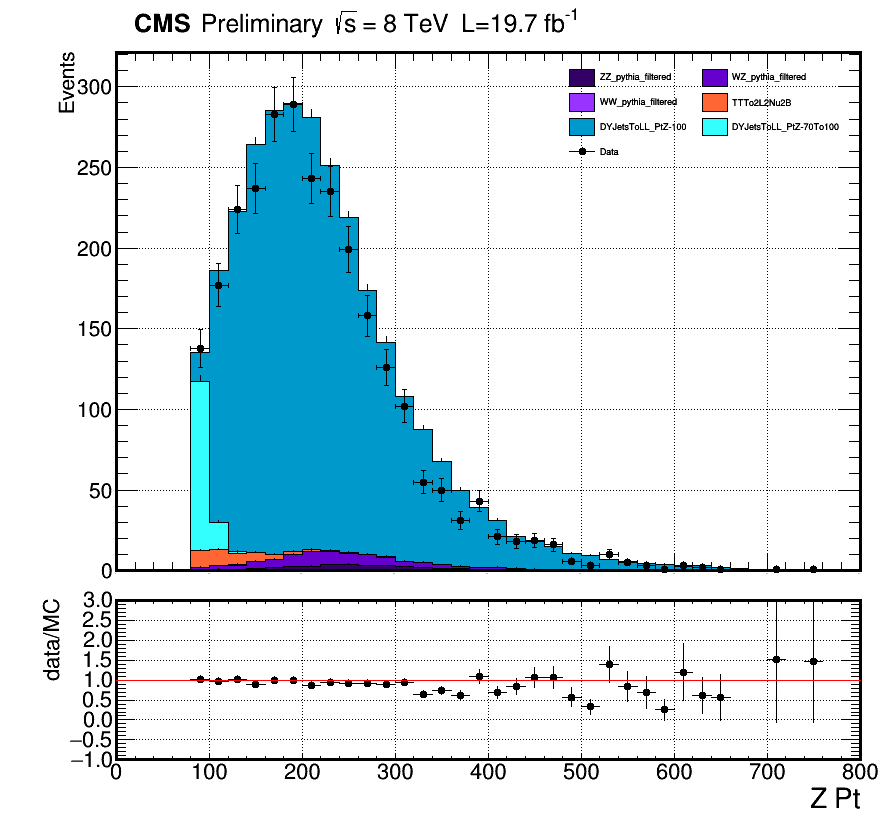
\includegraphics[scale=0.22]{figure/CH3/Z_kinematics/h_ZPt.png}}
  \caption{\label{fig:ZMassPt}Comparison between data and MC in SB region using mass and transverse momentum of reconstructed Z boson.}
\end{figure}

\begin{figure}[hbtp]
  \centering
  \subfigure[Z $\eta$]{
    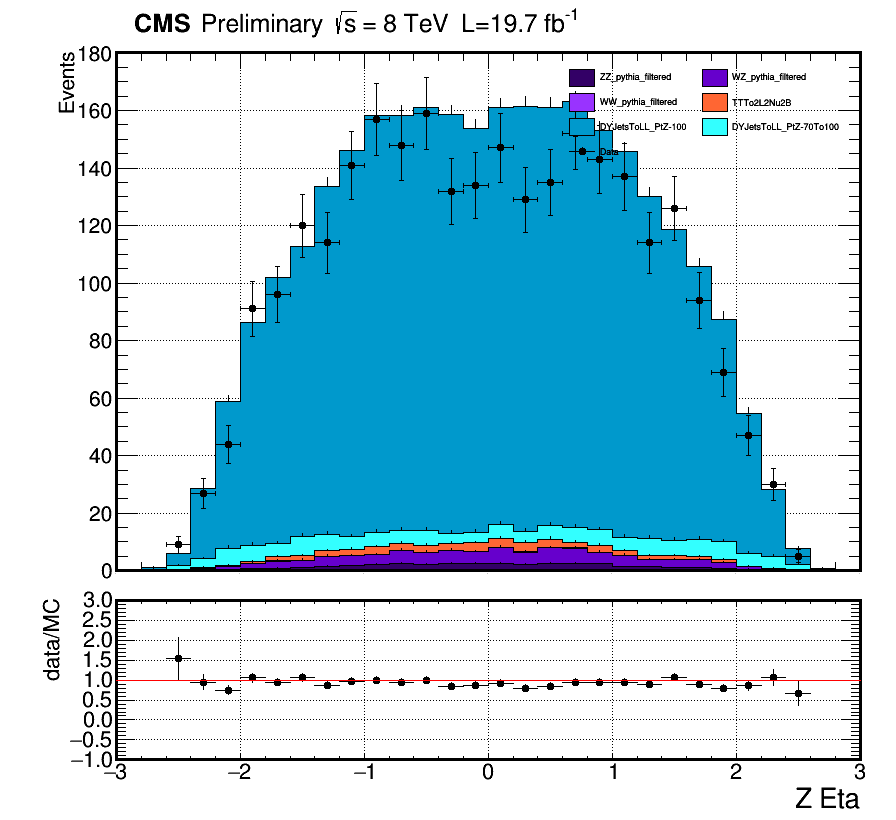
\includegraphics[scale=0.22]{figure/CH3/Z_kinematics/h_ZEta.png}}
  \hspace{0.5cm}
  \subfigure[Z $\phi$]{
    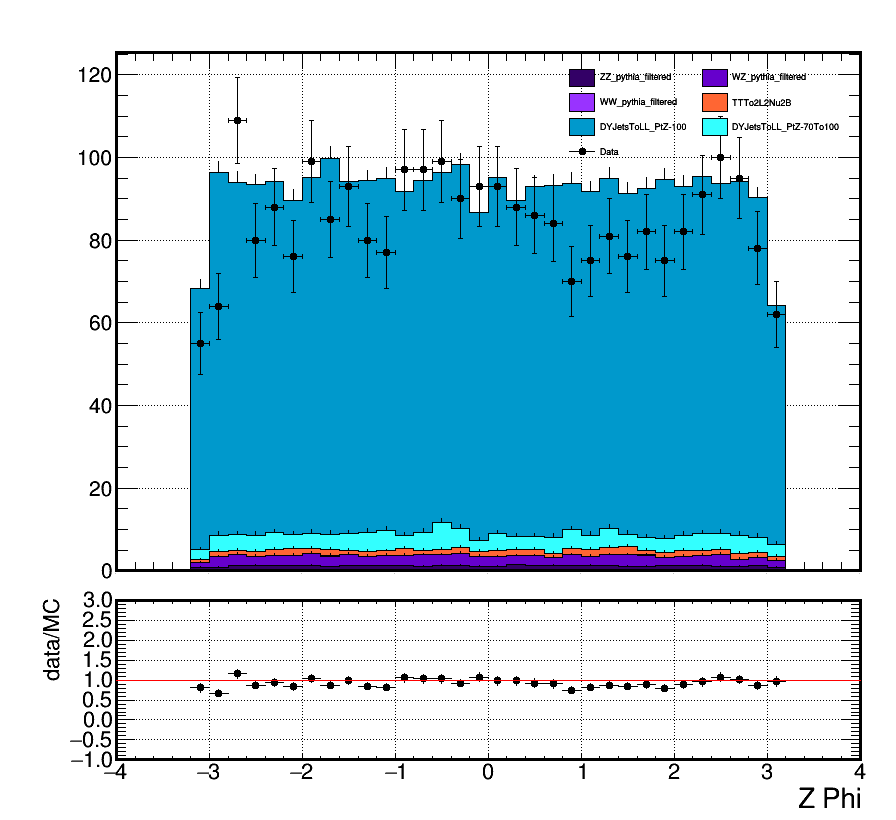
\includegraphics[scale=0.22]{figure/CH3/Z_kinematics/h_ZPhi.png}}
  \caption{\label{fig:ZEtaPhi}Comparison between data and MC in SB region using $\eta$ and $\phi$ of reconstructed Z boson.}
\end{figure}

\begin{figure}[hbtp]
  \begin{center}
    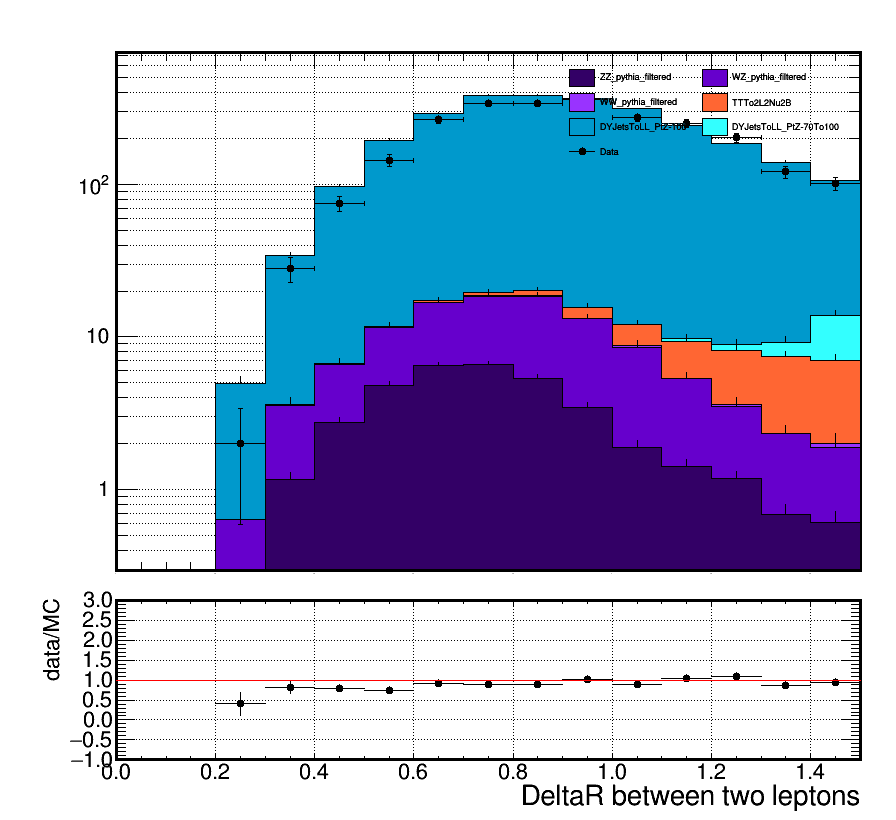
\includegraphics[width=0.5\textwidth]{figure/CH3/Z_kinematics/h_DeltaRll.png}
  \end{center}
  \caption{\label{fig:DeltaRll}$\Delta R$ between the two selected leptons.}
\end{figure}

\newpage
\section{Background Extrapolation}

The final aim of this analysis is to compare the predicted SM background with the observed data, it is important to elaborate a trustworthy strategy for the background estimation. Despite the good description of the event kinematics provided by the MC simulation, it is more advisable to minimize the dependence on the MC and develop a data driven strategy.

\subsection{$\alpha$ ratio method}

$\alpha$ ratio is a data driven method in order to estimate the final background in data signal region. We consider the $m_{Zh}$ MC mass spectrum in the SR and SB, then a ratio $\alpha$($m_{Zh}$) of the two is created. This factor $\alpha$ allows prediction of the mass spectrum in the signal region starting from the observed distribution in the sidebands. Under the assumption that this estrapolation from the sidebands to the signal region works in the same way both for data and MC, we can estimate the final background distribution in data signal region by multipling the $m_{Zh}$ mass spectrum observed in the sidebands by this $\alpha$ ratio:

\begin{align}
  \label{eq:AlphaRatio}
  N_{SR}^{data}(m_{Zh}) = N_{SB}^{data}(m_{Zh})\times \frac{N^{MC}_{SR}(m_{Zh})}{N^{MC}_{SB}(m_{Zh})}= N_{SB}^{data}(m_{Zh})\times \alpha (m_{Zh})
\end{align}

We divided the spectrum in 14 non-uniform width bins, as shown in Table~\ref{tab:bin}, accordingly to the decreasing statistics in the high mass tail.

\begin{center}
  \begin{table}[h]
    \begin{center}
      \begin{tabular}{c|c}
        \hline
        \bf Bin & \bf GeV \\
        \hline
        \hline
        1 & [680, 720] \\
        2 & [720, 760] \\
        3 & [760, 800] \\
        4 & [800, 840] \\
        5 & [840, 920] \\
        6 & [920, 1000] \\
        7 & [1000, 1100] \\
        8 & [1100, 1250] \\
        9 & [1250, 1400] \\
        10 & [1400, 1600] \\
        11 & [1600, 1800] \\
        12 & [1800, 2000] \\
        13 & [2000, 2200] \\
        14 & [2200, 2400] \\
        \hline
      \end{tabular}
    \end{center}
    \caption{\label{tab:bin}Binning of the Zh invariant mass range.}
  \end{table}
\end{center}

Finally, we multiplied the $\alpha$ ratio to the sidebands data $m_{Zh}$ distribution and obtained the prediction number of backgrounds in data signal region.

\begin{figure}[hbtp]
  \begin{center}
    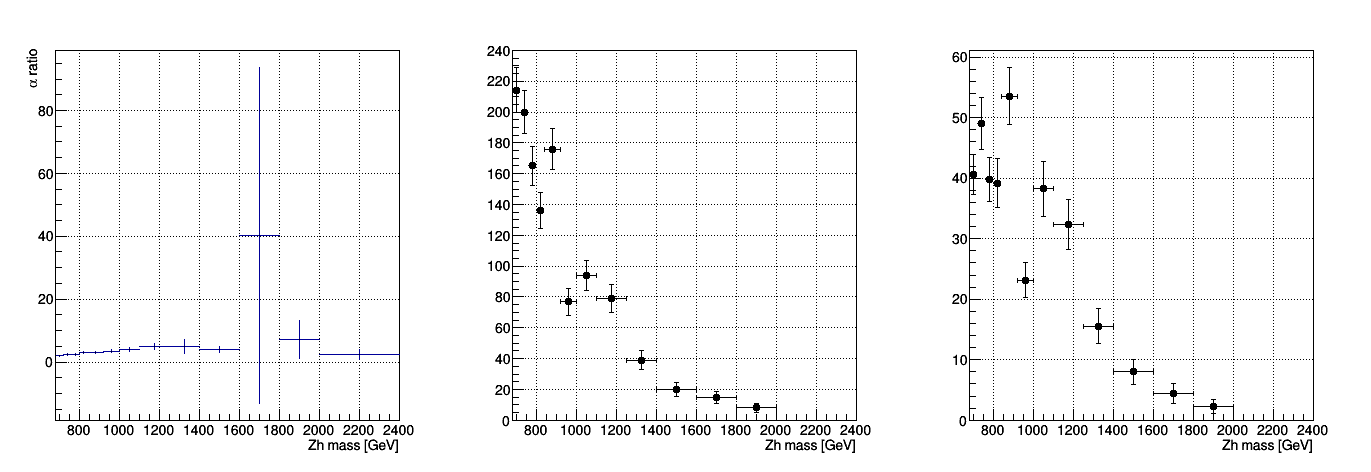
\includegraphics[width=\textwidth]{figure/CH3/alpha.png}
  \end{center}
  \caption{\label{fig:alpha}Left figure: the $\alpha$ ratio from MC simulation. Central figure: the $m_{Zh}$ distribution observed from data SB. Right figure: the predicted $m_{Zh}$ distribution in data signal region. }
\end{figure}


%% This textfile includes
% 3. Analysis procedures
%    ..
%    ..
%    3.9 Systematic uncertainties

\section{Systematic uncertainties}
The background and signal predictions are affected by systematic uncertainties that have to be estimated and taken into account for limit setting. This section includes a list of the relevant systematic uncertainties for this analysis and how they are estimated.

\begin{itemize}
\item \textbf{Luminosity:} The overall uncertainty of the LHC luminosity delivered to CMS in the 2012 Run-I is measured to be 2.6\%\cite{lumi}
\item \textbf{Jet energy scale:} The systematic on the jet energy scale was studied by scaling up and down the jet mass and $p_{T}$ according to the uncertainty associated to the jet energy corrections used. The Zh mass distributions reconstructed by jet four-momentum is affected and therefore we consider the shape uncertainty as well, shown in Fig.~\ref{fig:SYS_JES}. The overall uncertainty is about 8\%.
\end{itemize}

\begin{figure}[hbtp]
  \centering
  \subfigure[The systematic uncertainty of jet energy scale on background MC $m_{Zh}$ spectrum.]{
    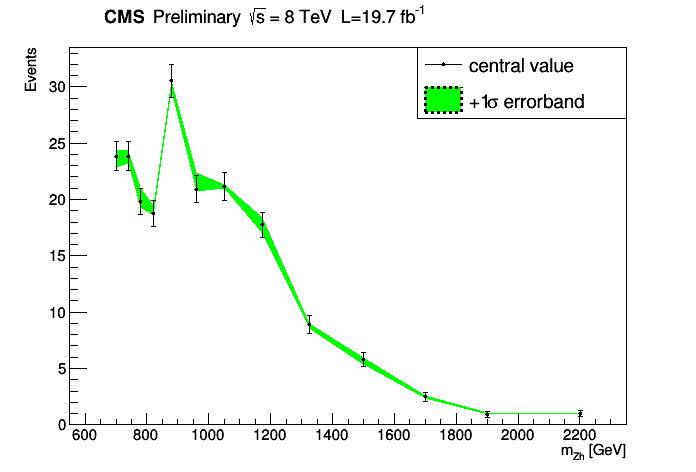
\includegraphics[scale=0.28]{figure/CH3/Systematics/Bkg_jes.png}}
  \hspace{0.5cm}
  \subfigure[The systematic uncertainty of jet energy scale on signal MC $m_{Zh}$ spectrum.]{
    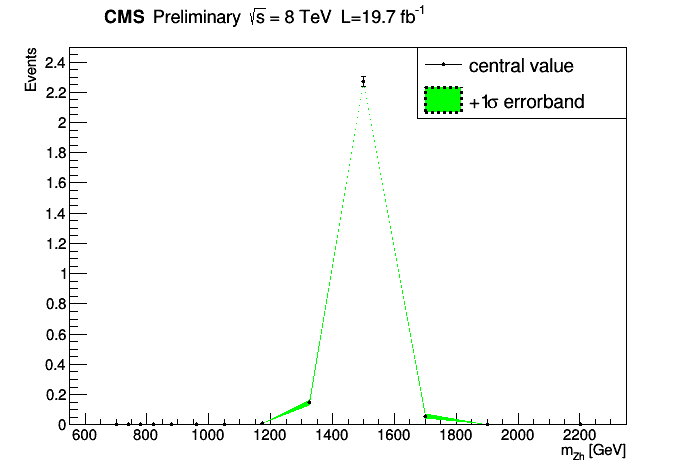
\includegraphics[scale=0.28]{figure/CH3/Systematics/Sig_jes.png}}
  \caption{\label{fig:SYS_JES}SR $m_{Zh}$ distributions for both signal (1500 GeV) and background MC samples. The uncertainty of jet energy scale is shown as the green error band ($\pm1 \sigma$), while the error bar presents the statistic error.}
\end{figure}

\begin{itemize}
\item \textbf{CSV distribution normalization:} The uncertainty comes when normalizing the CSV distributions of MC background prediction in order to match the data distribution, which is estimated about 10\%.
\item \textbf{Pile-up reweighting:} As described previously in section 3.4, we reweight the pile-up interactions in MC predictions for better modeling. To calculate the uncertainties on the pile-up simulation, we produce two pile-up distributions where the minimum bias cross section is shifted by $\pm$5\%\cite{PileupError}. The impact on the event yields is about 2\%. Despite the effects are small, we still consider it as the shape uncertainty. Fig.~\ref{fig:SYS_PU} shows the variation distributions of number of vertices for $\pm1\sigma$.  
\end{itemize}

\begin{figure}[hbtp]
  \centering
  \subfigure[Number of vertices in electron channel.]{
    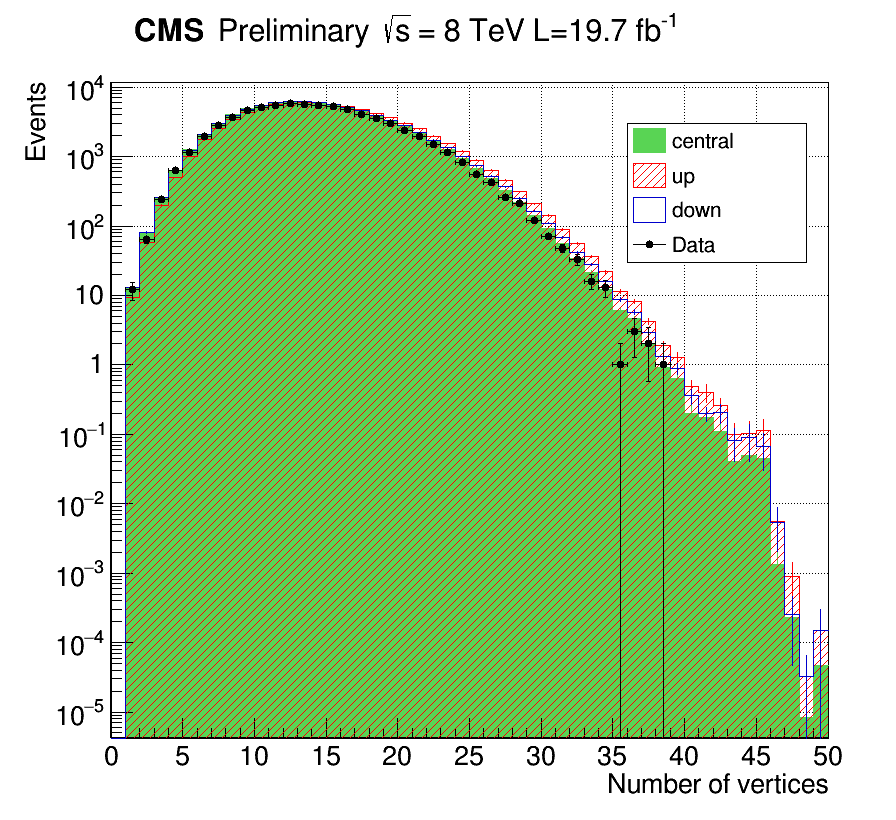
\includegraphics[scale=0.22]{figure/CH3/Systematics/h_nVtx_El_SysLog.png}}
  \hspace{0.5cm}
  \subfigure[Number of vertices in muon channel.]{
    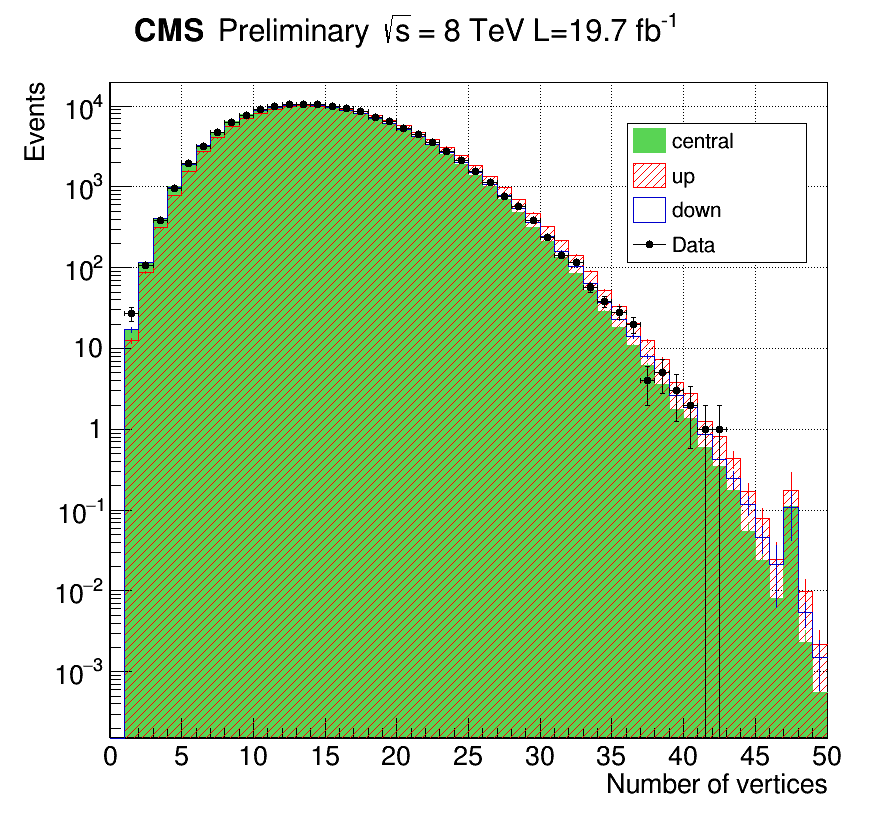
\includegraphics[scale=0.22]{figure/CH3/Systematics/h_nVtx_Mu_SysLog.png}}
  \caption{\label{fig:SYS_PU}(a) shows the distributions of number of vertices in electron channel, comparing central value of the total background prediction and the $\pm1\sigma$ variation, and data as well. (b) shows the result in muon channel.}
\end{figure}

\begin{itemize}
\item \textbf{Lepton ID scale factor:} The muon/electron ID scale factor depends on the kinematics of muon/electron (Table.~\ref{tab:lepIDsf}). This systematic was studied by applying $\pm 1 \sigma$ to the scale factor, the estimated uncertainty is 0.08\% for signal yields, 0.1\% for the Z+jets background, 0.05\% for $t\bar{t}$, and 0.06\% for the SM diboson backgrounds. No shape uncertainties are considered.
\item \textbf{b-jet Ratio:} Since the Drell-Yan process also generates b-jets into our background, the uncertainty of production cross section of Z+b-jets events indeed affects the number of background yield. The cross section ratio defined as $\sigma_{Z+bjet}$ divided by $\sigma_{Z+jet}$ and its uncertainties have been studied in \cite{SMP-13-004}. By scaling $1\sigma$ on the ratio, we etimated there's 0.2\% uncertainty for our Z+jets background yield.
\item \textbf{SHERPA:} The major background sample in this analysis is Z+jets, which is generated by MADGRAPH and showered by PYTHIA. In order to study the dependence on the MC generator, we use the Z+jets sample generated by SHERPA\cite{SHERPA} to estimate the background yield again. The relative uncertainty between SHERPA and MADGRAPH$\times$PYTHIA from the estimated background yield is taken as the systematic by 12\%.
\item \textbf{Diboson cross section:} Uncertainties of the SM WW/WZ/ZZ production cross section affect their estimated background yield about 5.4\%/6.7\%/5.5\%.
\item \textbf{PDF uncertainty:} Systematic uncertainties coming from different choice of PDF sets have been considered for this analysis. This study is performed by varing the PDF set when producing the signal samples. The default PDF set we used is CTEQ6L1, replaced by the following PDF set: MSTW2008lo, MSTW2008nlo, NNPDF21\_lo, NNPDF21\_nlo and CT10. Comparison of distributions from different PDF sets are shown in Fig.~\ref{fig:StackPDF}. The estimated overall uncertainty for signal yields is 12\% (maximum), shape uncertainty is also taken into account.
\end{itemize}

\begin{center}
  \begin{table}[h]
    \begin{center}
      \begin{tabular}{|c|c|c|c|c|}
        \hline
        electron $p_{T}$ [GeV] & $0.0 < |\eta| < 0.8$ & $0.8 < |\eta| < 1.442$ & $1.556 < |\eta| < 2.0$ & $2.0 < |\eta| < 2.5$\\ \hline
        20-30 & 1.005 $\pm$ 0.003 & 0.981 $\pm$ 0.003 & 0.980 $\pm$ 0.005 & 1.017 $\pm$ 0.006\\
        30-40 & 1.004 $\pm$ 0.001 & 0.991 $\pm$ 0.001 & 0.992 $\pm$ 0.002 & 1.019 $\pm$ 0.003\\
        40-50 & 1.008 $\pm$ 0.001 & 0.994 $\pm$ 0.001 & 1.004 $\pm$ 0.002 & 1.005 $\pm$ 0.001\\
        50-200 & 1.008 $\pm$ 0.001 & 0.999 $\pm$ 0.001 & 1.006 $\pm$ 0.003 & 1.009 $\pm$ 0.002\\
        \hline
      \end{tabular}
      \begin{tabular}{|c|c|c|c|}
        \hline
        muon $p_{T}$ [GeV] & $0.0 < |\eta| < 0.8$ & $0.8 < |\eta| < 2.1$ & $2.1 < |\eta| < 2.4$\\ \hline
        20-40 & 1.0043 $\pm$ 0.0004 & 1.0074 $\pm$ 0.0005 & 1.022 $\pm$ 0.001  \\
        40-100 & 1.0012 $\pm$ 0.0004 & 1.0043 $\pm$ 0.0004 & 1.014 $\pm$ 0.001 \\
        \hline
      \end{tabular}
    \end{center}
    \caption{\label{tab:lepIDsf}Data to simulation scale factors for muon and electron identification requirements in various $p_{T}$ and $\eta$ ranges.}
  \end{table}
\end{center}

\begin{figure}[hbtp]
  \centering
  \subfigure[$m_{Zh}$ spectrum of 800 GeV $Z'$ sample]{
    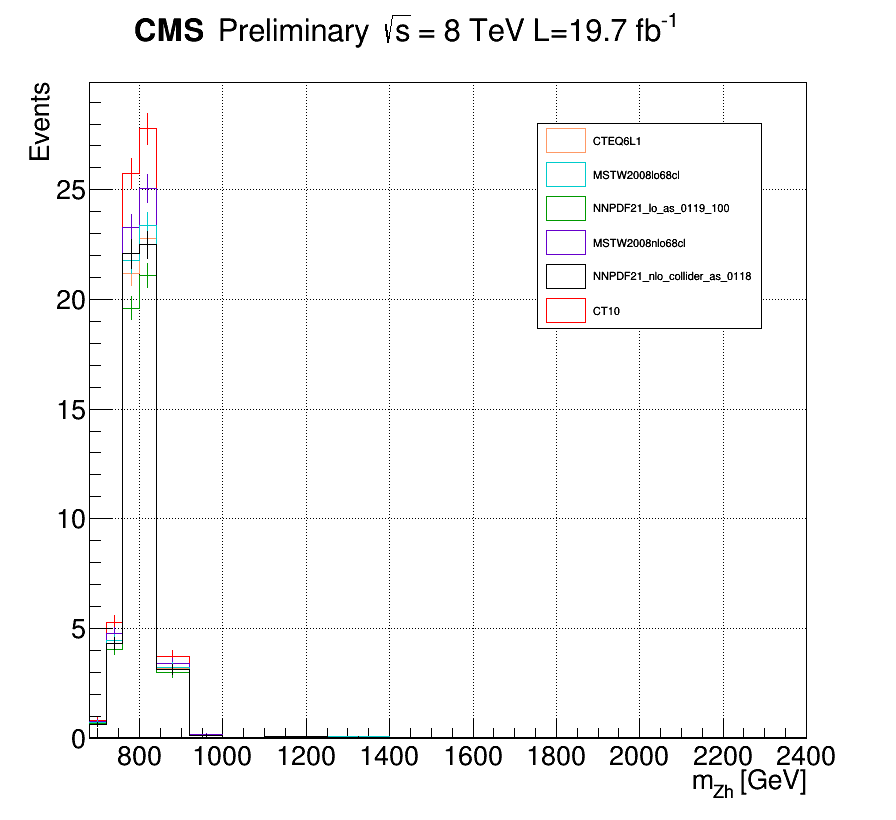
\includegraphics[scale=0.22]{figure/CH3/Systematics/StackPDF_M800.png}}
  \hspace{0.5cm}
  \subfigure[CSV shape of 800 GeV $Z'$ sample]{
    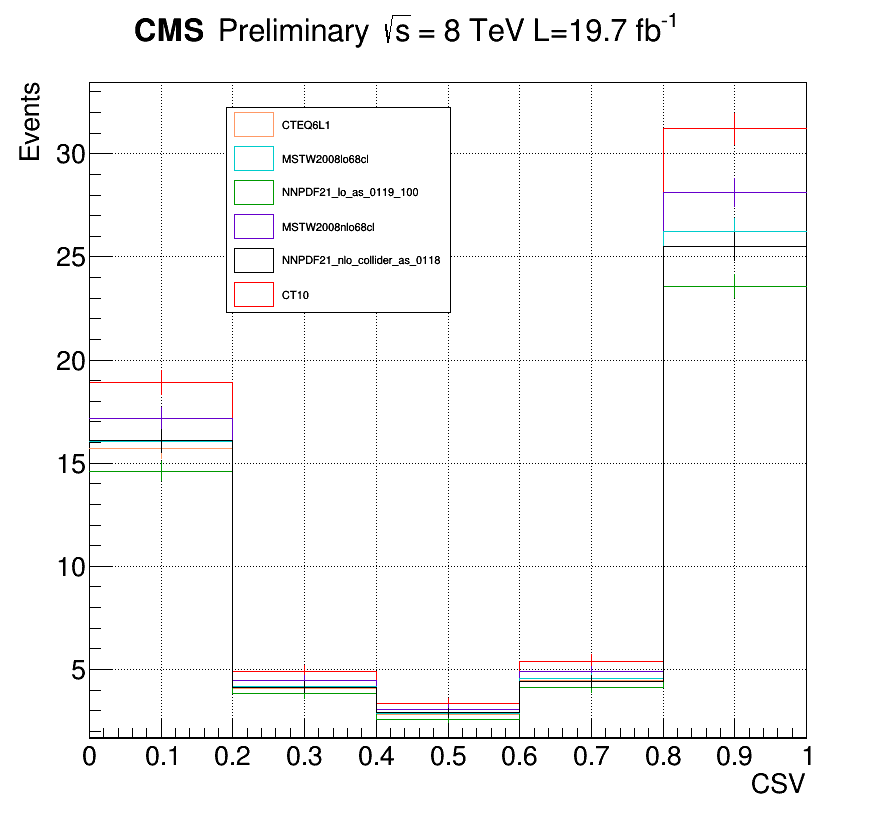
\includegraphics[scale=0.22]{figure/CH3/Systematics/StackCSV_M800.png}}
  \hspace{0.5cm}
  \subfigure[$m_{Zh}$ spectrum of 1200 GeV $Z'$ sample]{
    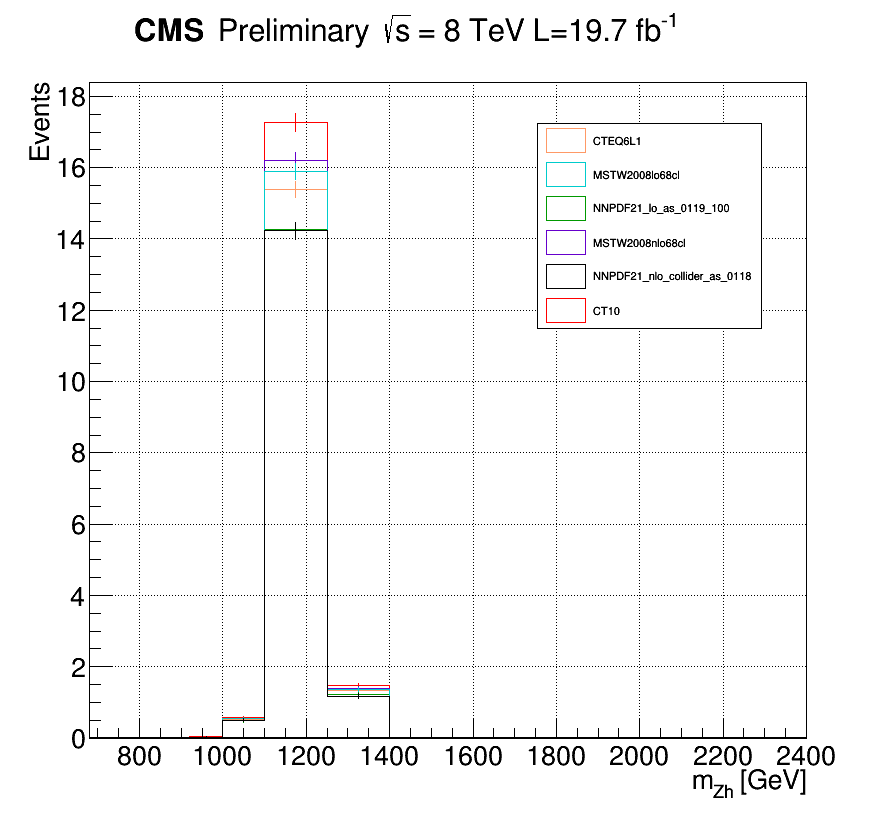
\includegraphics[scale=0.22]{figure/CH3/Systematics/StackPDF_M1200.png}}
  \hspace{0.5cm}
  \subfigure[$m_{Zh}$ spectrum of 2000 GeV $Z'$ sample]{
    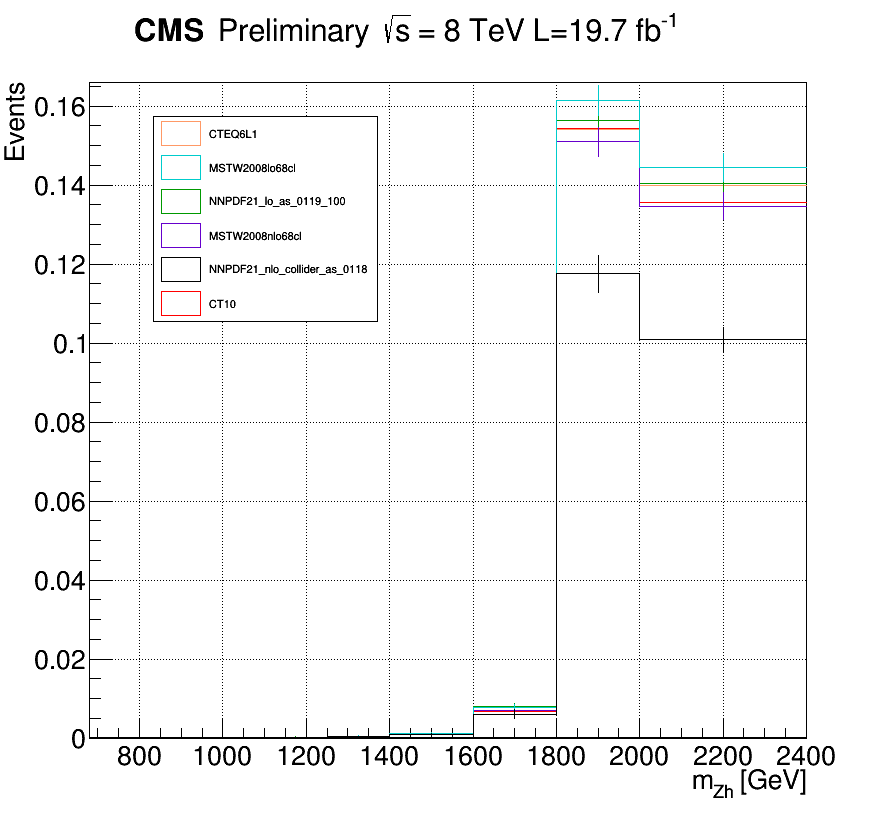
\includegraphics[scale=0.22]{figure/CH3/Systematics/StackPDF_M2000.png}}
  \caption{\label{fig:StackPDF} The comparison between different PDF sets using $m_{Zh}$ spectrum and CSV variable.}
\end{figure}

%\chapter{Results and conclusion}
In this chapter, the final selection is finally applied. The signal, background, and data count after this selection is then be used to perform the estimation of upper limits of excited leptons. This chapter also make comparisons to $\mu\mu^{*}\rightarrow 4\mu$ and $ee^{*}\rightarrow 4e$ channels. In the end, the final excited muon limit is shown by combining the results of $\mu\mu^{*}\rightarrow 2\mu 2e$ and $\mu\mu^{*}\rightarrow 4\mu$ channels, and the same is done for limit of excited electron.    

\section{Cross section limit computation}

As no significant excess can be observed, there is no evidence for existence of excited leptons. Thus, the sight now turns to set the limit for the excludable signal cross section as well as the region in the space of the excited lepton mass to the compositness scale parameter $\Lambda$. The calculation of the $95 \%$ CL excluded cross section is done with a Bayesian approach by using the statistical tool provided by the CMS collaboration that is based on ROOSTATS \cite{RooStatsCl95, stat_HiggsPAG}.

The statistical analysis of each channel is performed as a single bin counting experiment that is performed for each signal point individually. The two channels of e* and $\mu^{*}$ respectively are afterward combined to a single limit in order to further expand the excluded region. 

\section{Optimization of the final selection}

\label{sec:optimization}For our final selection, we look at the minimum-maximum three-body invariant mass plane. The signal has the shape of an inverted L in this plane. By adding a minimum invariant mass cut (vertical, left area) and a maximum invariant mass cut (horizontal, above area), the background can be discriminated  easily. Fig. \ref{fig:MminMmaxSignal} shows the minimum-maximum invariant mass plane for both $\mu\mu^{*}\rightarrow 2\mu 2e$ and $ee^{*}\rightarrow 2e2\mu$ channels with different invariant masses. 

\begin{figure}[hp]
\begin{center}
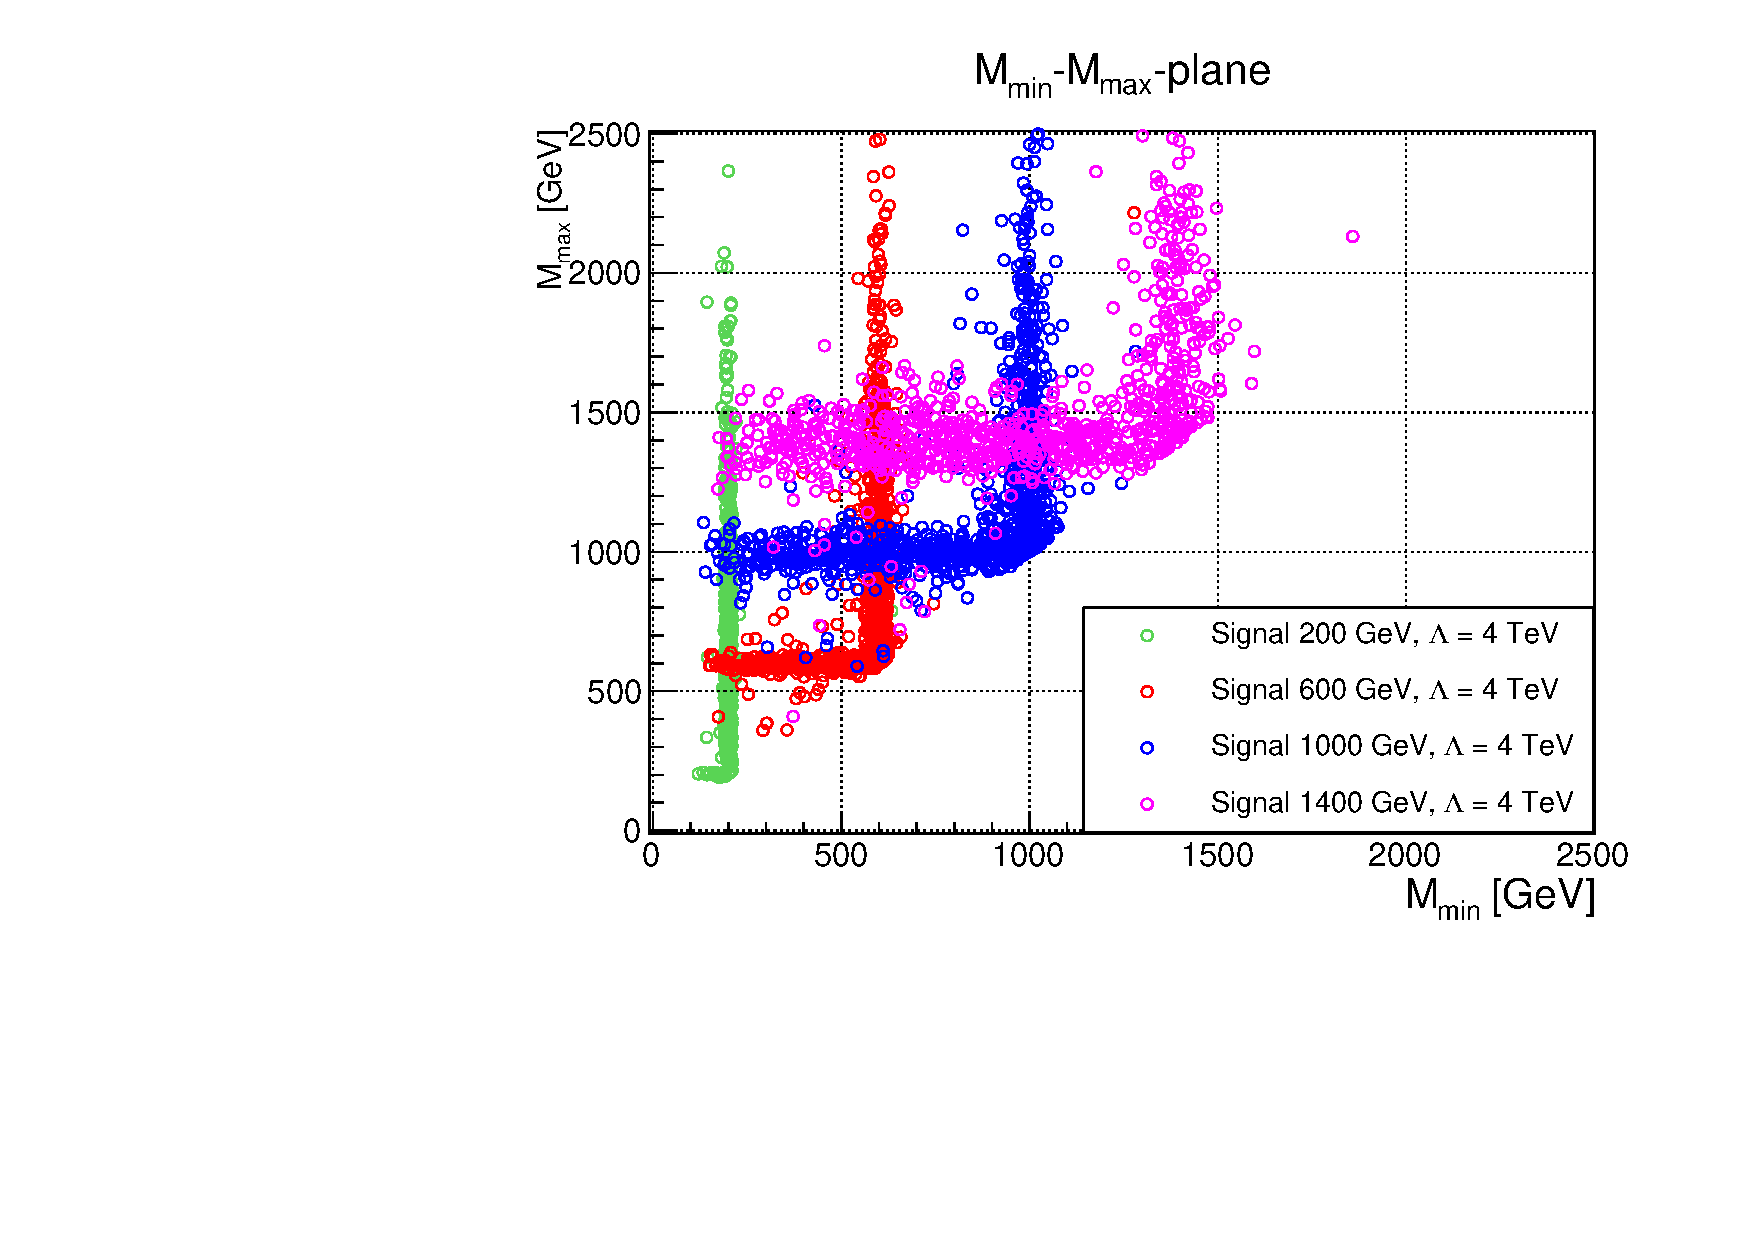
\includegraphics[width=0.48\textwidth]{plot/signal_2mu2e.pdf} 
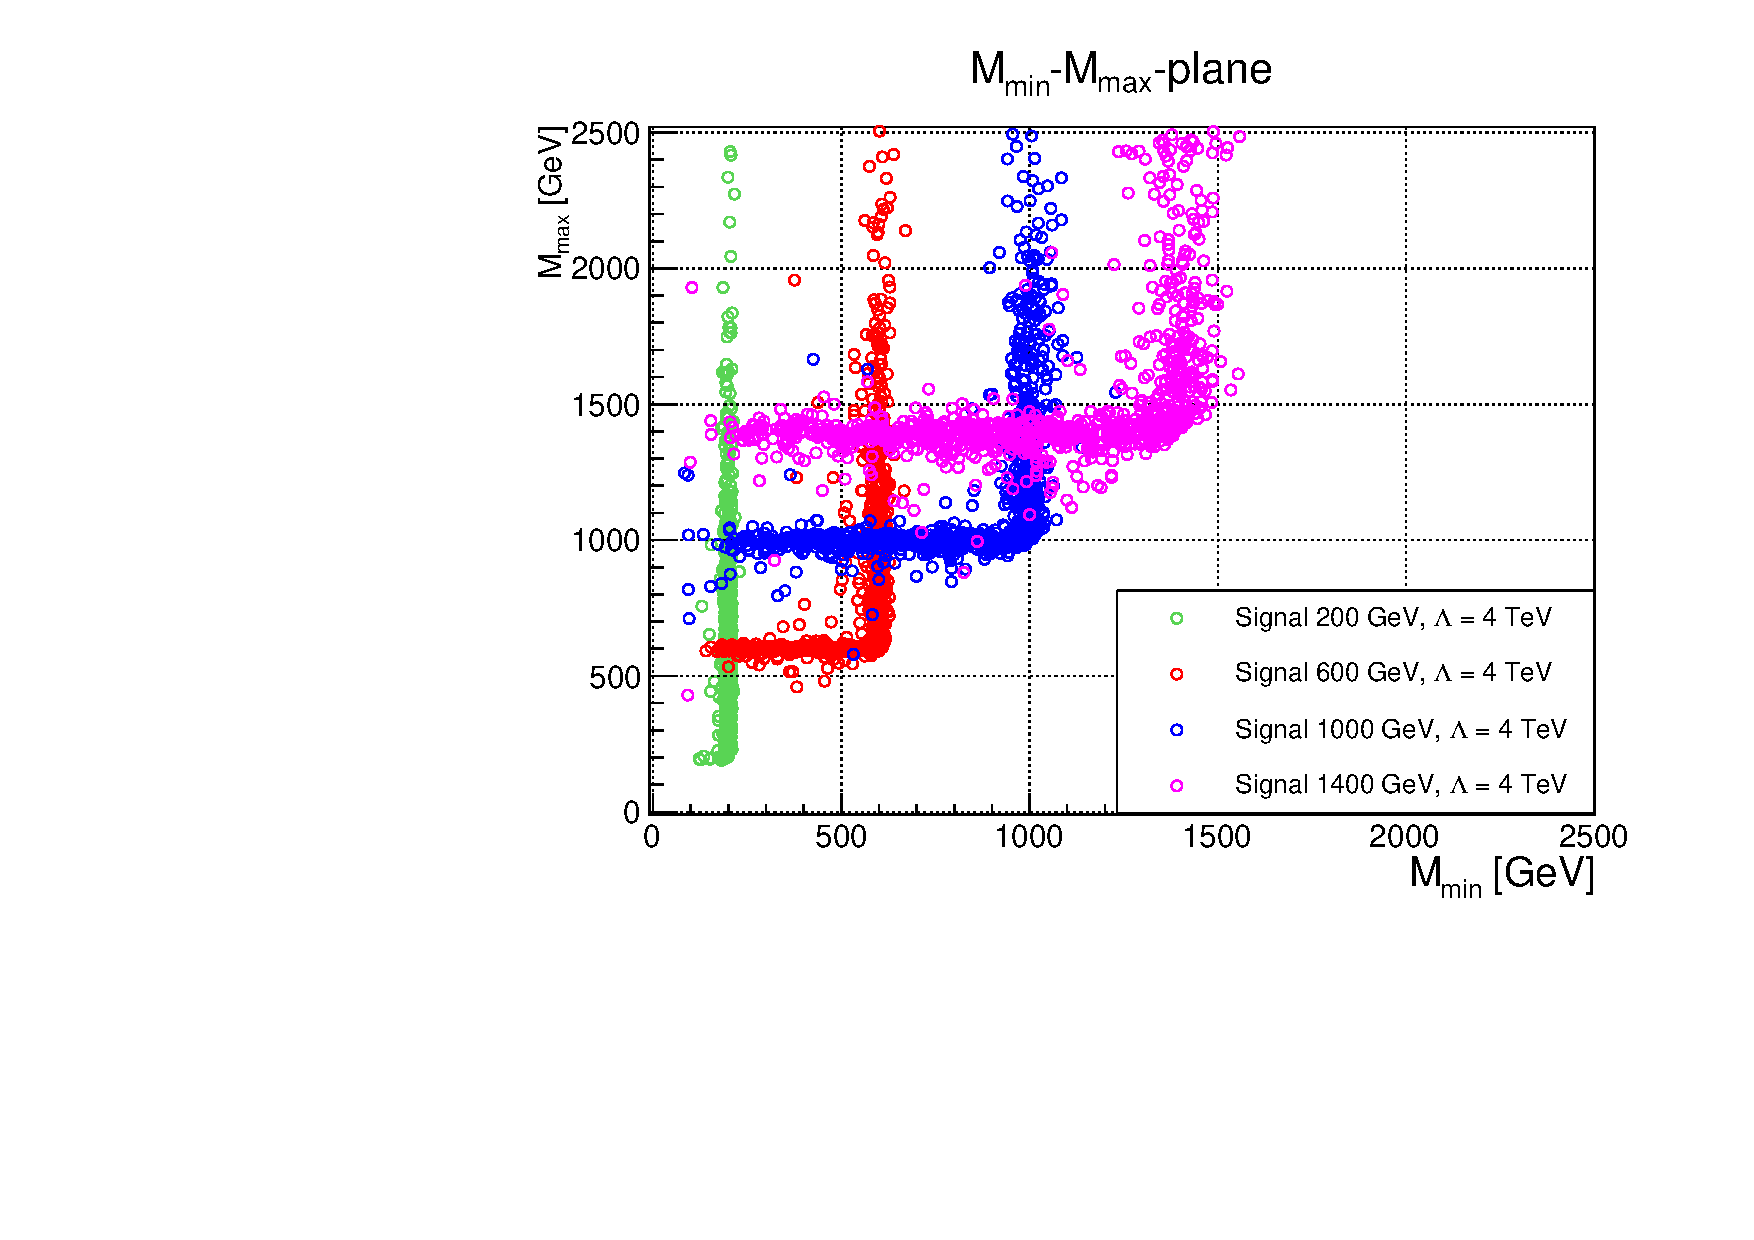
\includegraphics[width=0.48\textwidth]{plot/signal_2e2mu.pdf}
\end{center}
\caption{\label{fig:MminMmaxSignal}2-dimensional minimum-maximum invariant mass distribution after invariant mass cuts for different $l^{*}$ masses. Left: $\mu\mu^{*}\rightarrow 2\mu 2e$ channel. Right: $ee^{*}\rightarrow 2e2\mu$ channel.}
\end{figure}

The boundaries of the final selection depend on the mass of the excited leptons. Fig. \ref{fig:Boundaries} shows the selection of the boundaries for an invariant mass of 600 GeV. There are four cuts set: A lower cut von $M_{min}$, a higher cut on $M_{min}$, a lower cut on $M_{max}$ and a higher cut on $M_{max}$. The most important cuts of this four are the higher $M_{min}$ and the lower $M_{max}$ cuts, which do most effort on seperating signal and background. For the definition of the cut ranges, the best expected limit for the lower maximum invariant mass cut was calculated. Now, a range from optimized lower $M_{max}$ cut to the central mass of each $l^{*}$ samples is obtained. Then, we apply this range to upper $M_{max}$ cut, upper $M_{min}$ cut, and lower $M_{min}$ cut to form a symmetric signal region for each signal sample. Tab. \ref{tab:LShape2} - \ref{tab:LShape4} show the range and the event yields for the different $l^{*}$ masses and Fig. \ref{fig:Efficiencies_L} shows the acceptance $\times$ efficiency after lepton selection, after the Z-veto selection and after the final selection.

\begin{figure}
 \begin{center}
  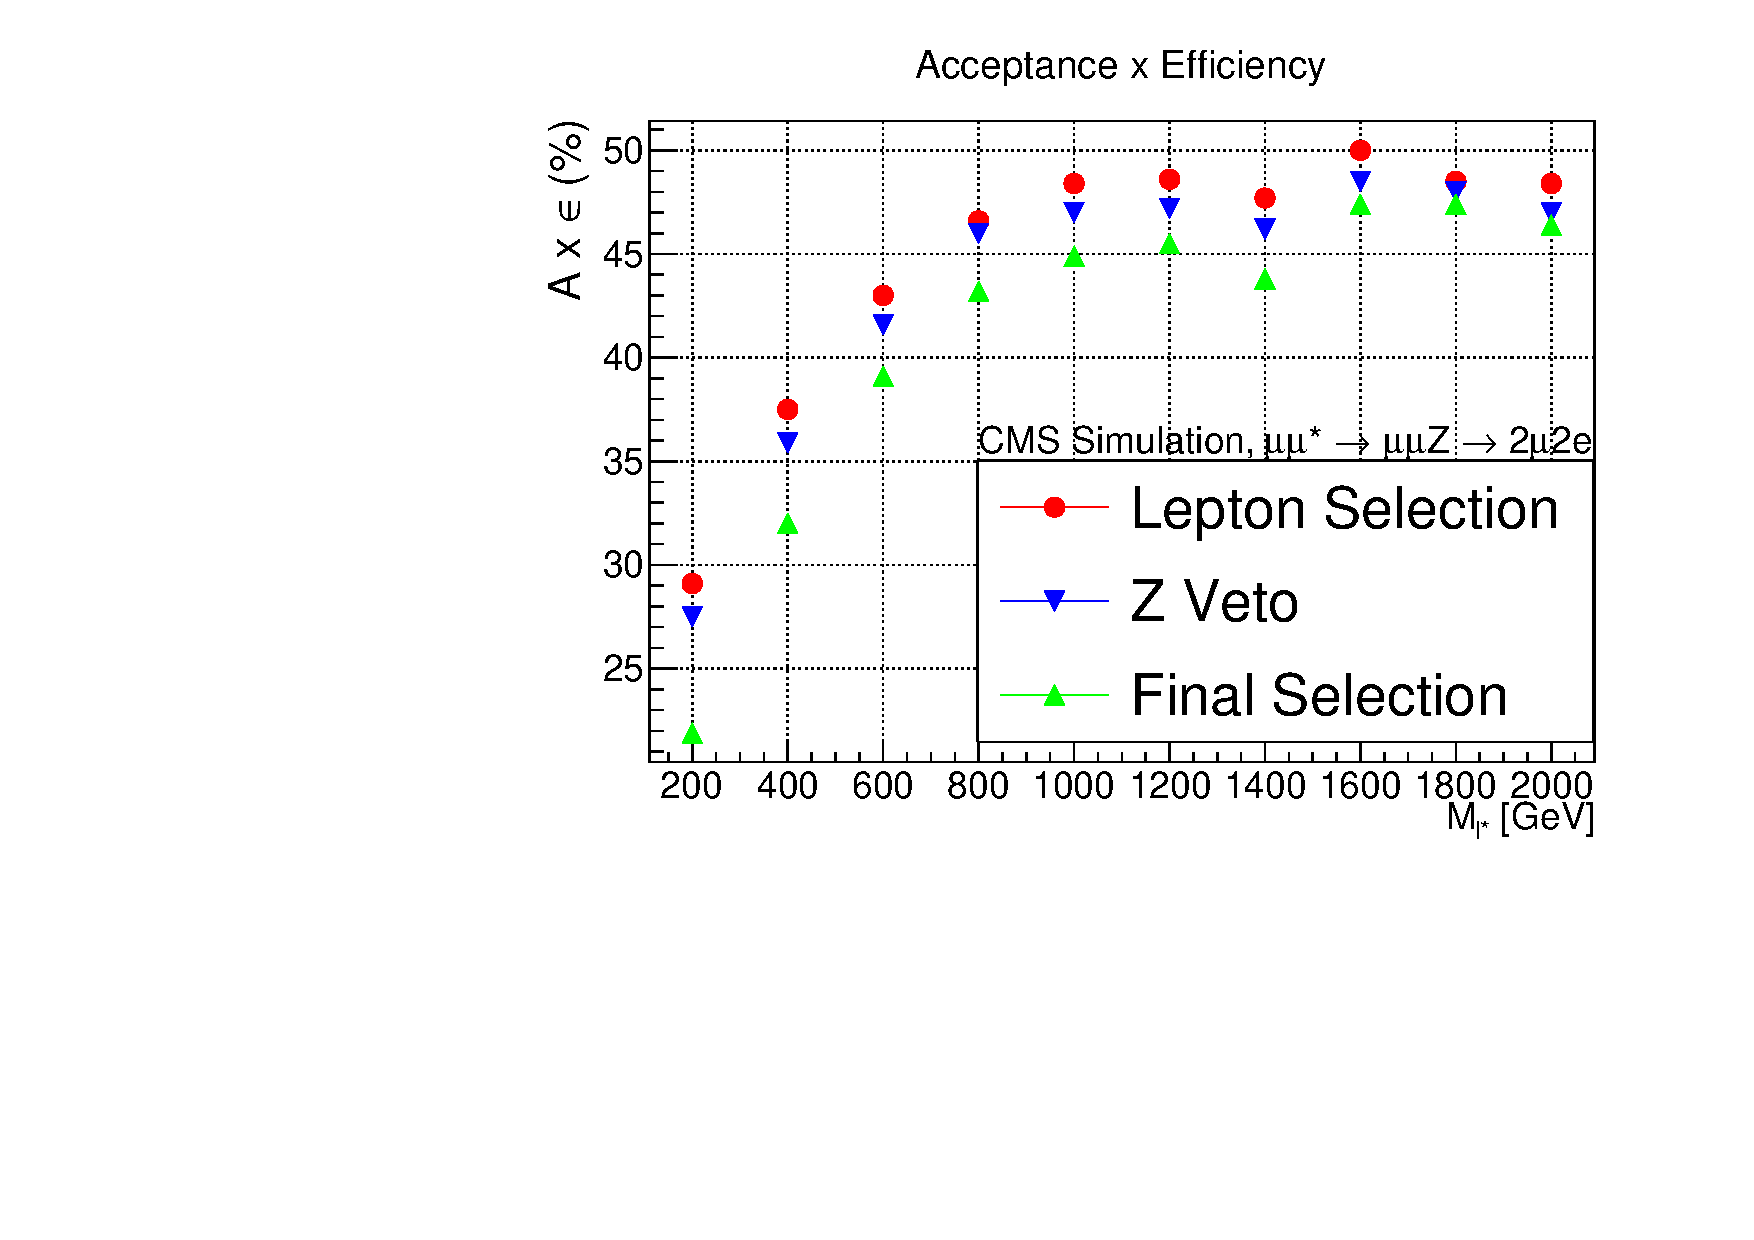
\includegraphics[width=0.48\textwidth]{plot/Effizienz_2mu2e.pdf}
  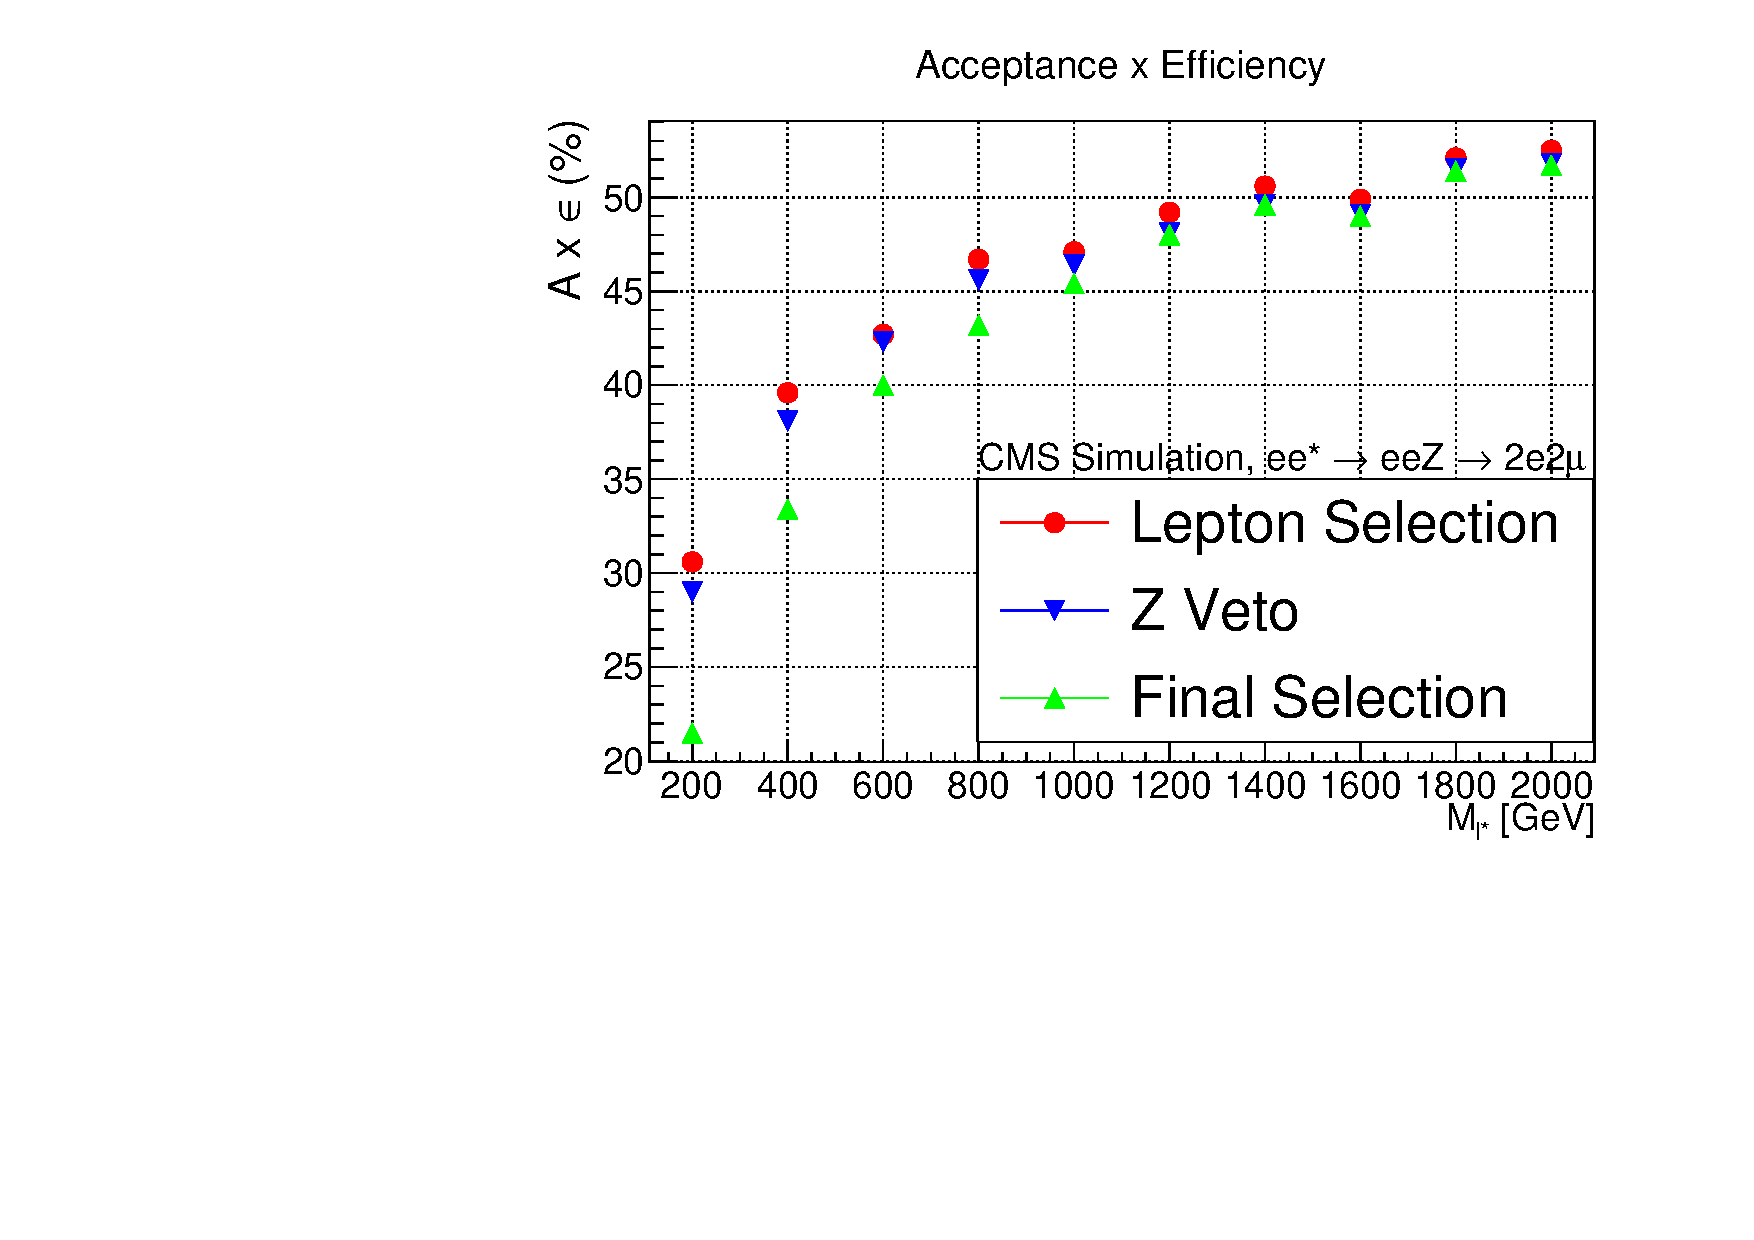
\includegraphics[width=0.48\textwidth]{plot/Effizienz_2e2mu.pdf}
 \end{center}
\caption{\label{fig:Efficiencies_L}Acceptance $\times$ Efficiency for different cut stages: Lepton selection, Z veto and final selection. }
\end{figure}



\begin{table}[h!]
\begin{center}
\begin{tabular}{|l|c|c|c|c|c|}
\hline
m($\mu^{*}$) [GeV] & $M_{min}-M_{max}$ Cut [GeV] & Data & BG (\# Events) & $\epsilon_{all}$ \\
\hline
\hline
200 & 196-204 & 0 & 0.23 $\pm$ 0.05 & 22.3\% \\
400 & 376-424 & 1 & 0.14$\pm$ 0.03 & 32.8\% \\
600 & 540-660 & 0 & 0.07 $\pm$ 0.03 & 39.8\% \\
800 & 720-880 & 0 & 0.04 $\pm$ 0.01 & 44.3\% \\
1000 & 850-1150 & 0 & 0.01 $\pm$ 0.01 & 46.1\% \\
1200 & 1000-1400 & 0 & 0.00 $\pm$ 0.00 & 46.7\% \\
1400 & 1200-1800 & 0 & 0.01 $\pm$ 0.01 & 45.0\% \\
1600 & 1200-2200 & 0 & 0.01 $\pm$ 0.01 & 48.4\% \\
1800 & 1200-2600 & 0 & 0.01 $\pm$ 0.01 & 48.7\% \\
2000 & 1200-3000 & 0 & 0.01 $\pm$ 0.01 & 47.6\% \\
2200 & 1200-3400 & 0 & 0.01 $\pm$ 0.01 & 47.4\% \\
2400 & 1200-3800 & 0 & 0.01 $\pm$ 0.01 & 48.2\% \\
2600 & 1200-4200 & 0 & 0.01 $\pm$ 0.01 & 45.5\% \\
\hline
\end{tabular}
\caption{\label{tab:LShape2}Cut ranges for the L shape cuts, corresponding event yields and signal efficiencies $\mu\mu^{*} \rightarrow 2\mu 2e$.}
\end{center}
\end{table} 

\begin{table}[h!]
\begin{center}
\begin{tabular}{|l|c|c|c|c|c|}
\hline
m($e^{*}$) [GeV] & $M_{min}-M_{max}$ Cut [GeV] & Data & BG (\# Events) & $\epsilon_{all}$ \\
\hline
\hline
200 & 196-204 & 0 & 0.24 $\pm$ 0.05 & 22.4\% \\
400 & 384-416 & 0 & 0.09 $\pm$ 0.02 & 34.6\% \\
600 & 552-648 & 0 & 0.08 $\pm$ 0.02 & 41.6\% \\
800 & 728-872 & 0 & 0.02 $\pm$ 0.01 & 44.7\% \\
1000 & 860-1140 & 0 & 0.02 $\pm$ 0.01 & 47.3\% \\
1200 & 860-1540 & 0 & 0.02 $\pm$ 0.01 & 49.7\% \\
1400 & 860-1940 & 0 & 0.02 $\pm$ 0.01 & 51.1\% \\
1600 & 860-2340 & 0 & 0.02 $\pm$ 0.01 & 51.1\% \\
1800 & 860-2740 & 0 & 0.02 $\pm$ 0.01 & 53.7\% \\
2000 & 860-3140 & 0 & 0.02 $\pm$ 0.01 & 53.8\% \\
2200 & 860-3540 & 0 & 0.02 $\pm$ 0.01 & 52.3\% \\
2400 & 860-3940 & 0 & 0.02 $\pm$ 0.01 & 52.8\% \\
2600 & 860-4340 & 0 & 0.02 $\pm$ 0.01 & 52.6\% \\
\hline
\end{tabular}
\caption{\label{tab:LShape4}Cut ranges for the L shape cuts, corresponding event yields and signal efficiencies $e e^{*} \rightarrow 2e 2\mu$.}
\end{center}
\end{table} 


\begin{figure}[hp]
\begin{center}
\includegraphics[width=0.48\textwidth]{plot/L_shape_2mu2e.pdf} 
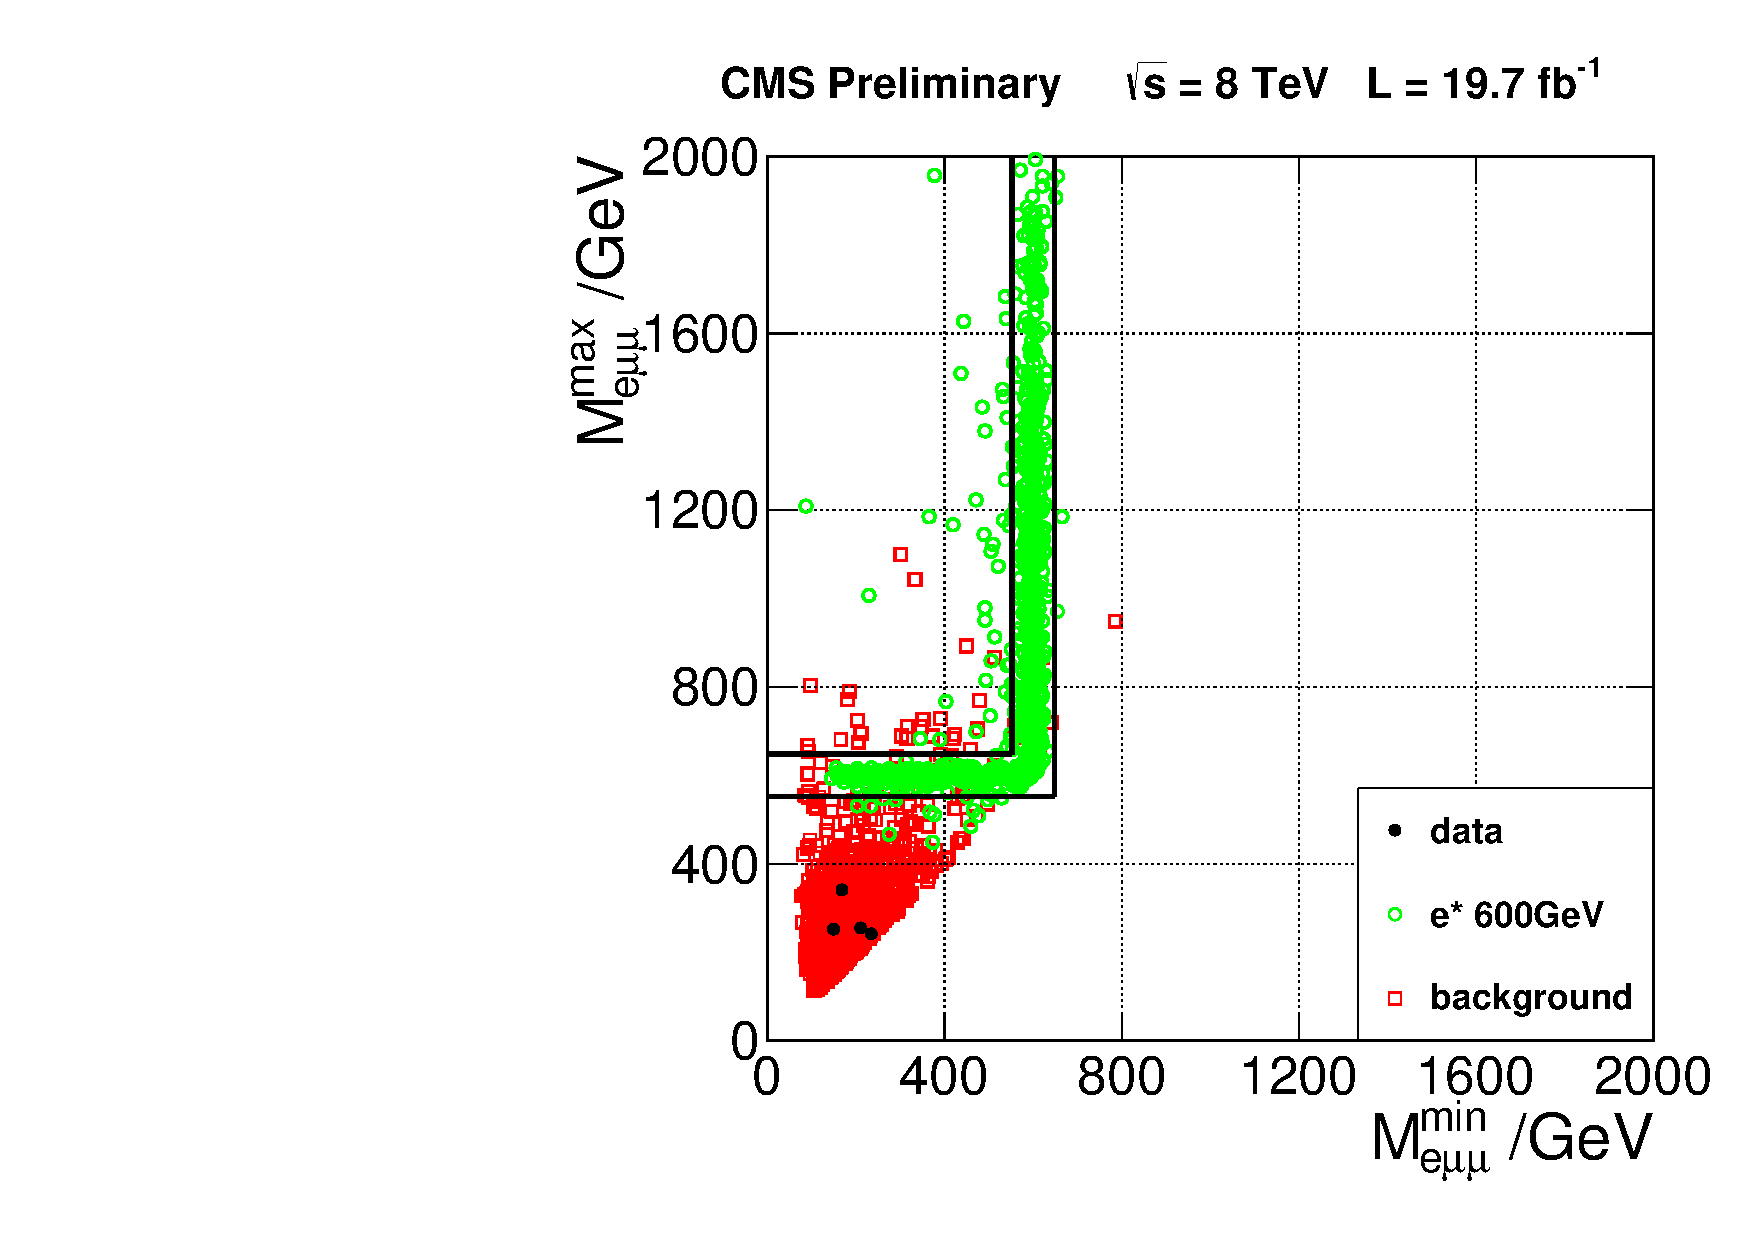
\includegraphics[width=0.48\textwidth]{plot/L_shape_2e2mu.pdf}
\end{center}
\caption{\label{fig:Boundaries}2-dimensional minimum-maximum invariant mass distribution after invariant mass cuts. Left: $\mu\mu^{*} \rightarrow 2\mu 2e$ channel. Right: $ee^{*}\rightarrow 2e2\mu$ channel.}
\end{figure}


Looking at the Tab. \ref{tab:LShape2}-\ref{tab:LShape4}, it can be seen that the selected signal regions do not cover the complete parameter space. Especially in the low mass regions, there are gaps between the search regions that might lead to a case where a potential excited lepton could not be discovered. Those gaps are closed by additional L-shaped search regions that are determined as follows. The 4e-channel is chosen to estimate the new regions as it has the best mass resolution and thus the most narrow windows. For the windows given by the signal MC, the width was plotted depending on the $e^*$-Mass. The width and the position of the new windows is estimated by linear interpolation. The positions are used in all channels, while the correponding width has to be estimated for each channel individually.

Measured data, as well as the background expectation in this new search regions can be drived from the distribution. As there is no corresponding MC, this information is not available for the signal. Estimate the signal contribution by a fit on the points we have from the signal MC. 

The channels containing muons have a much higher A x $\epsilon$ because of the higher efficiency of the high-$p_{T}$ muon ID. As the numbers show, the lose of efficiency due to the L shape cut is very small while we can discriminate the background to a small amount of events. This characteristic returns a very good signal over brackground ratio. 


\section{Limit computation}

The selection defined in section \ref{sec:optimization} and the limit setting tool are used to calculate observed and expected limits for all four channels. The inputs from Tab. \ref{tab:LShape2} - \ref{tab:LShape4} are used for the limit calculation. The calculated cross section limits depend on the compositeness scale $\Lambda$ (here, $f = f^{\prime} = 1$ is assumed). One natural point for limit setting is the point where the $l^{*}$-mass and the compositeness scale have the same value.      

\subsection{Limits for excited muons $\mu^{*}$}

Fig. \ref{fig:limit4mu} and \ref{fig:limit2mu2e} show the cross section limits and the limits on the compositeness scale for $\mu\mu^{*}\rightarrow 4\mu$ and $\mu\mu^{*} 
\rightarrow 2\mu2e$ depending on the $\mu^{*}$-mass. The black lines show the signal cross section for different values of $\Lambda$. From those plots, the channel 
$\mu\mu^{*}\rightarrow 4\mu$ excited muons can be excluded up to a mass of 1.65 TeV for $\Lambda = M_{\mu^{*}}$. In the channel  $\mu\mu^{*}\rightarrow 2\mu2e$, the limit is set to 1.60 TeV. 

\begin{figure}[hp!]
\begin{center}
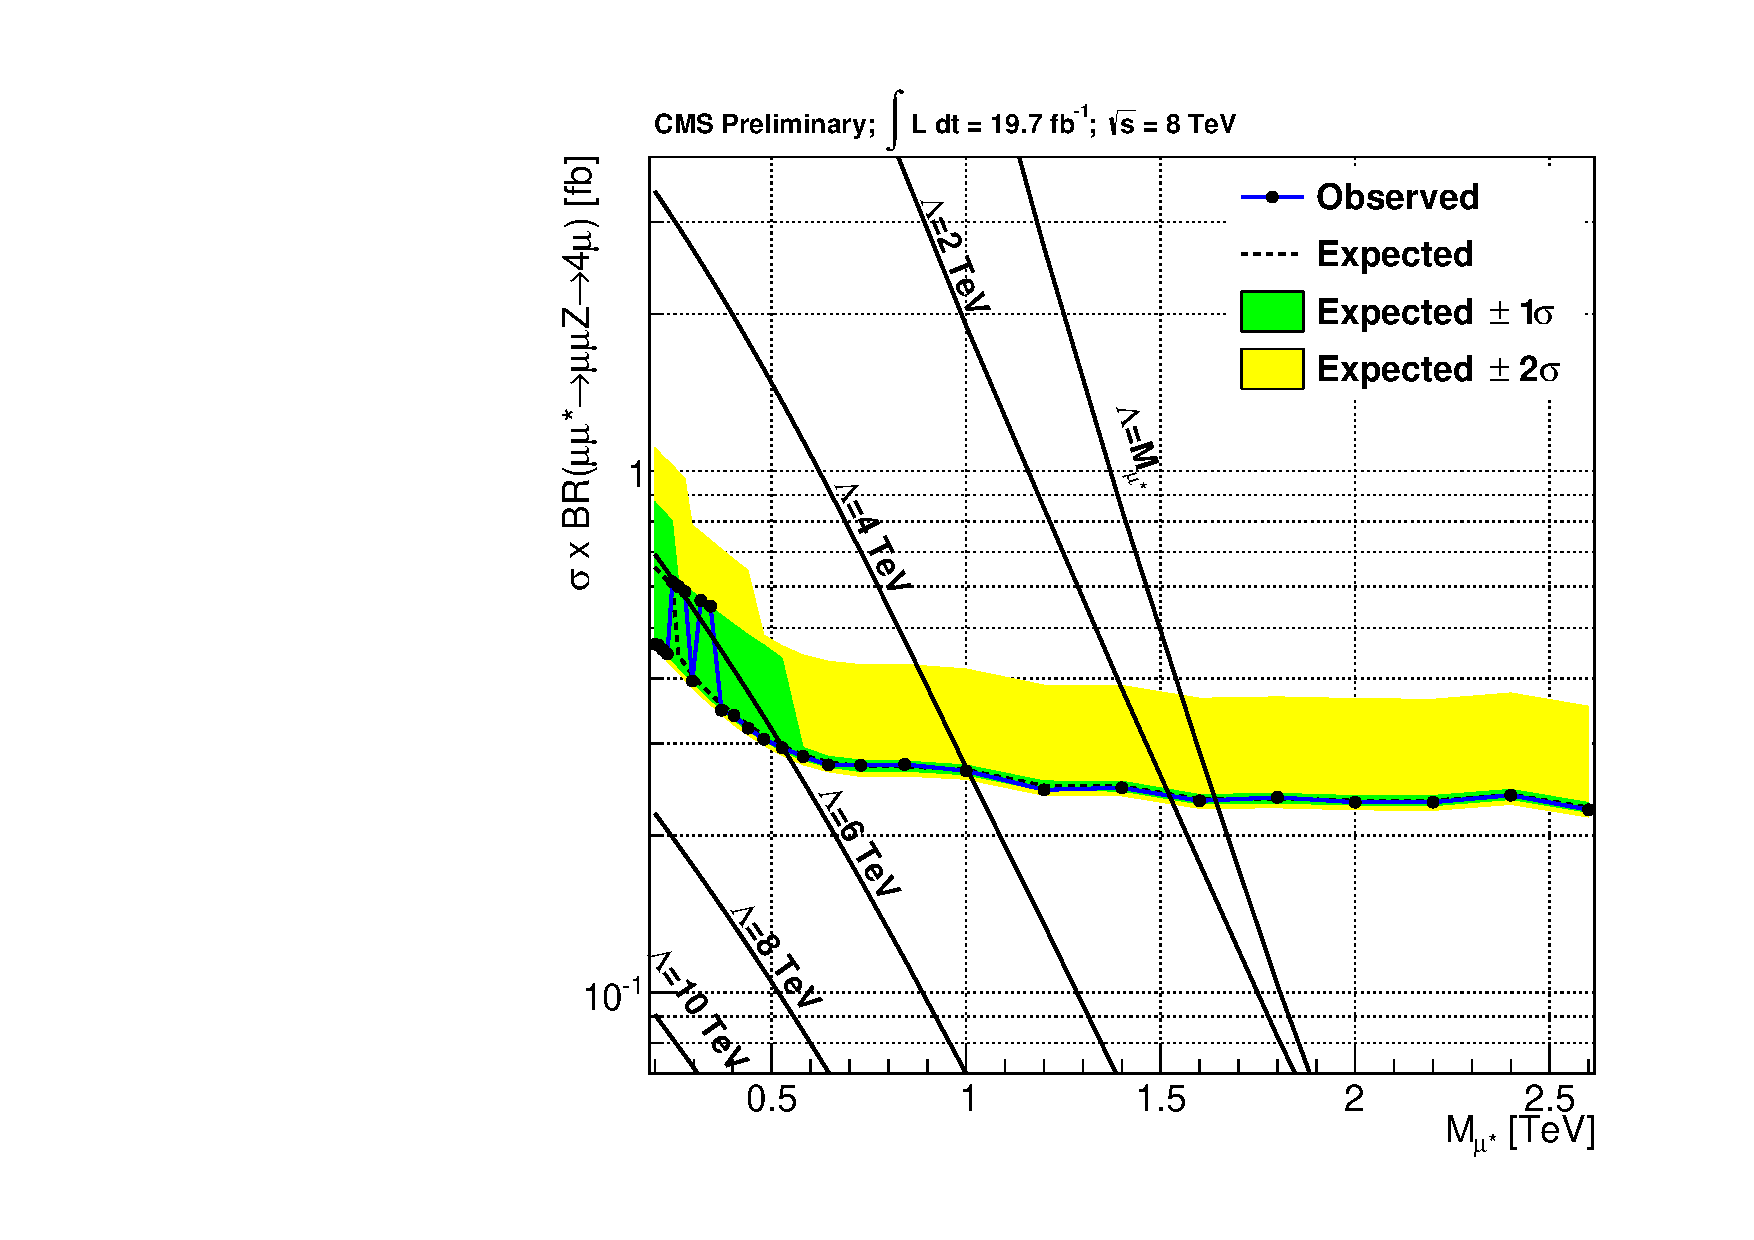
\includegraphics[width=0.48\textwidth]{plot/limit_4mu.pdf}
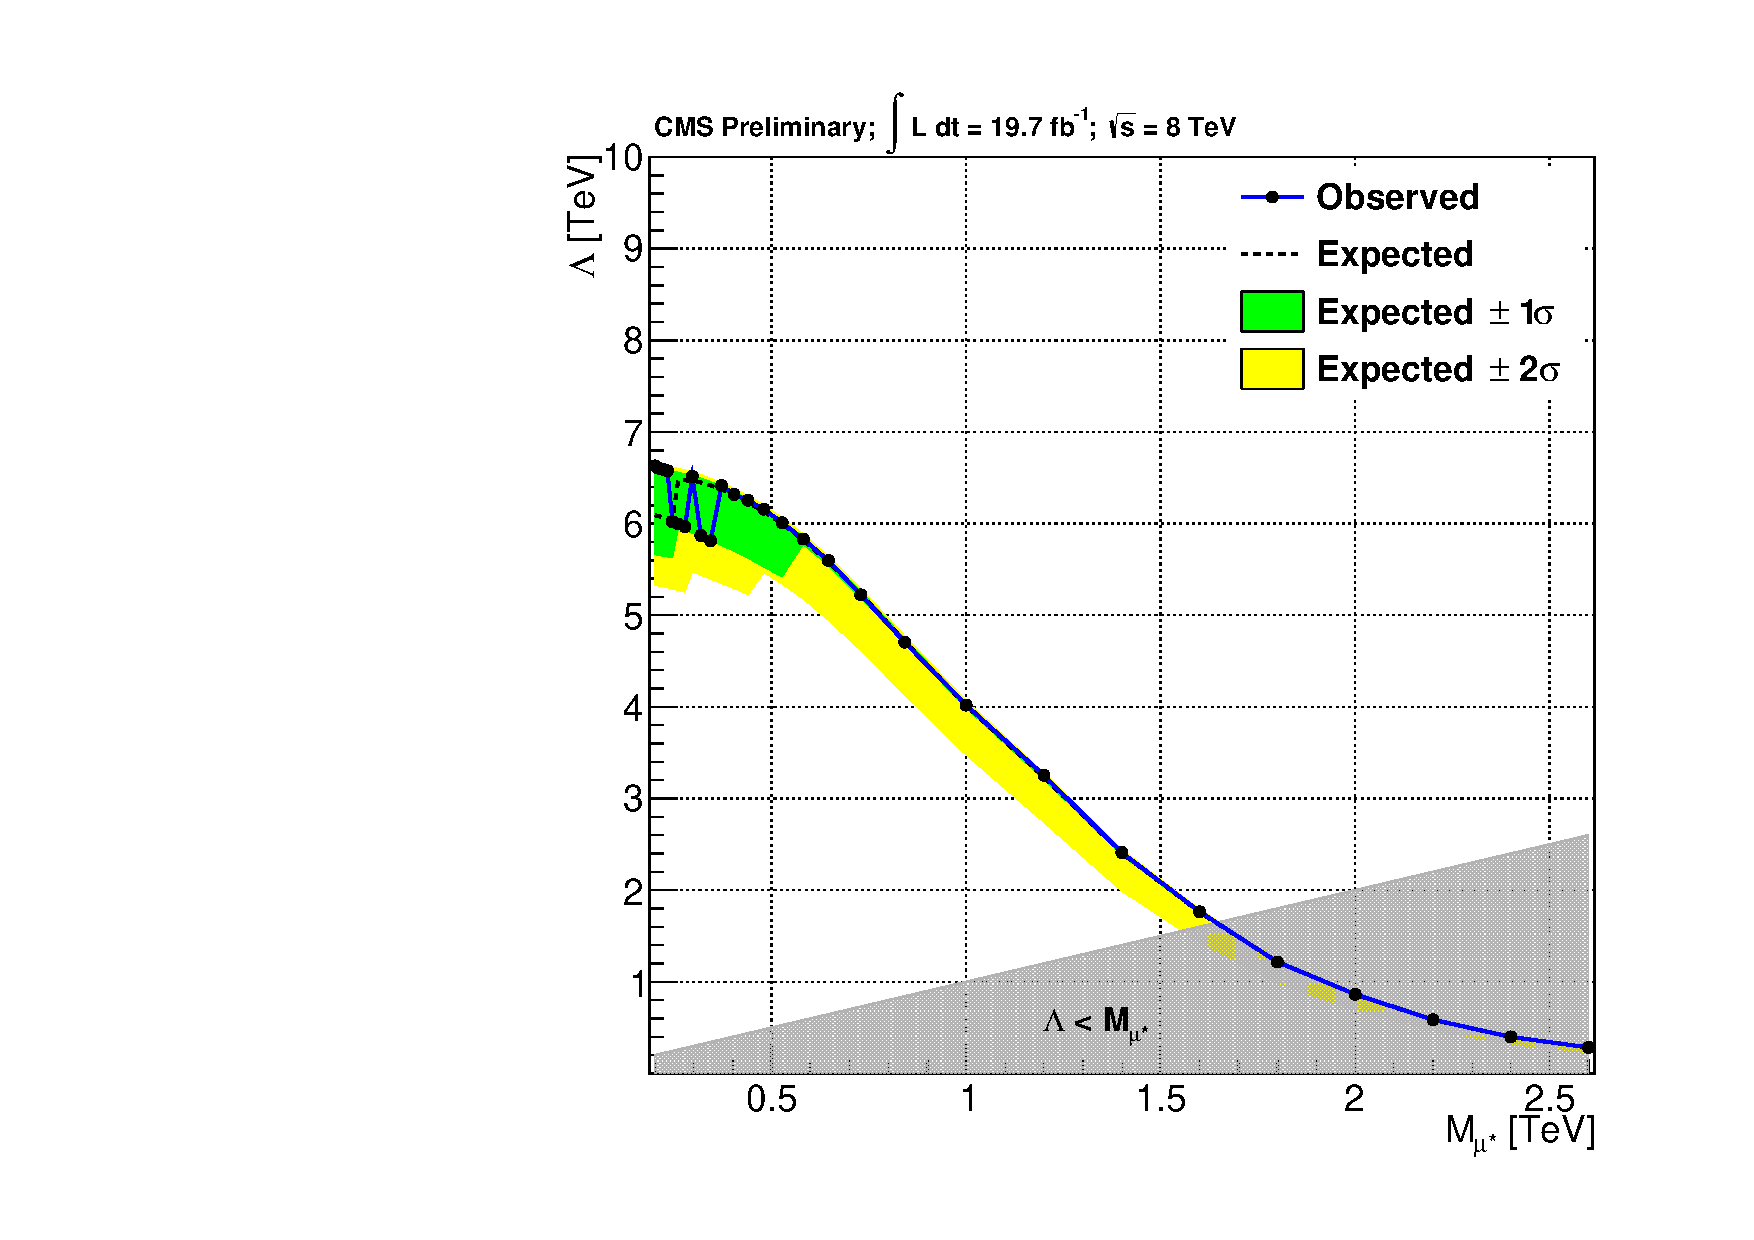
\includegraphics[width=0.48\textwidth]{plot/limit_lambda_4mu.pdf}
\end{center}
\caption{\label{fig:limit4mu}Cross section and $\Lambda$ limit for $\mu\mu^{*} \rightarrow 4\mu$.}
\end{figure}

\begin{figure}[hp!]
\begin{center}
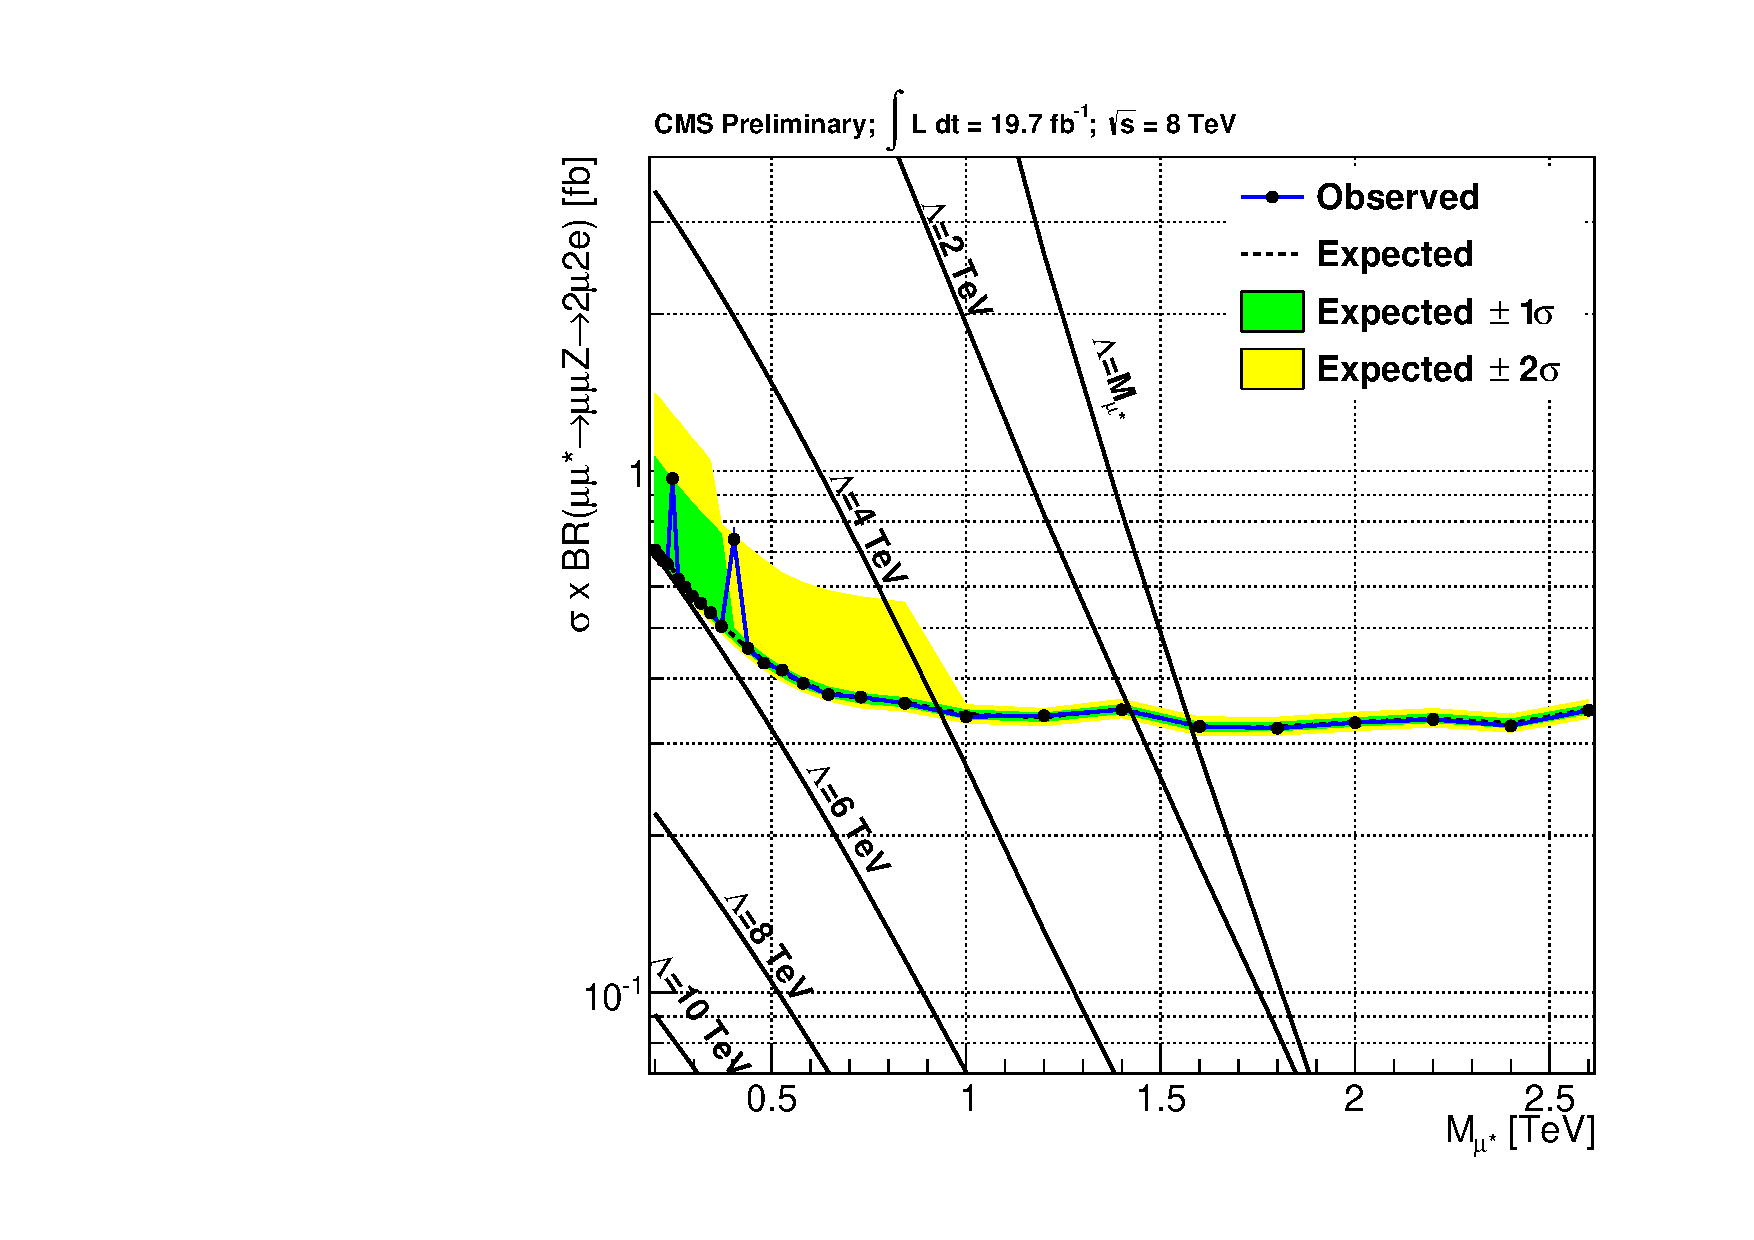
\includegraphics[width=0.48\textwidth]{plot/limit_2mu2e.pdf}
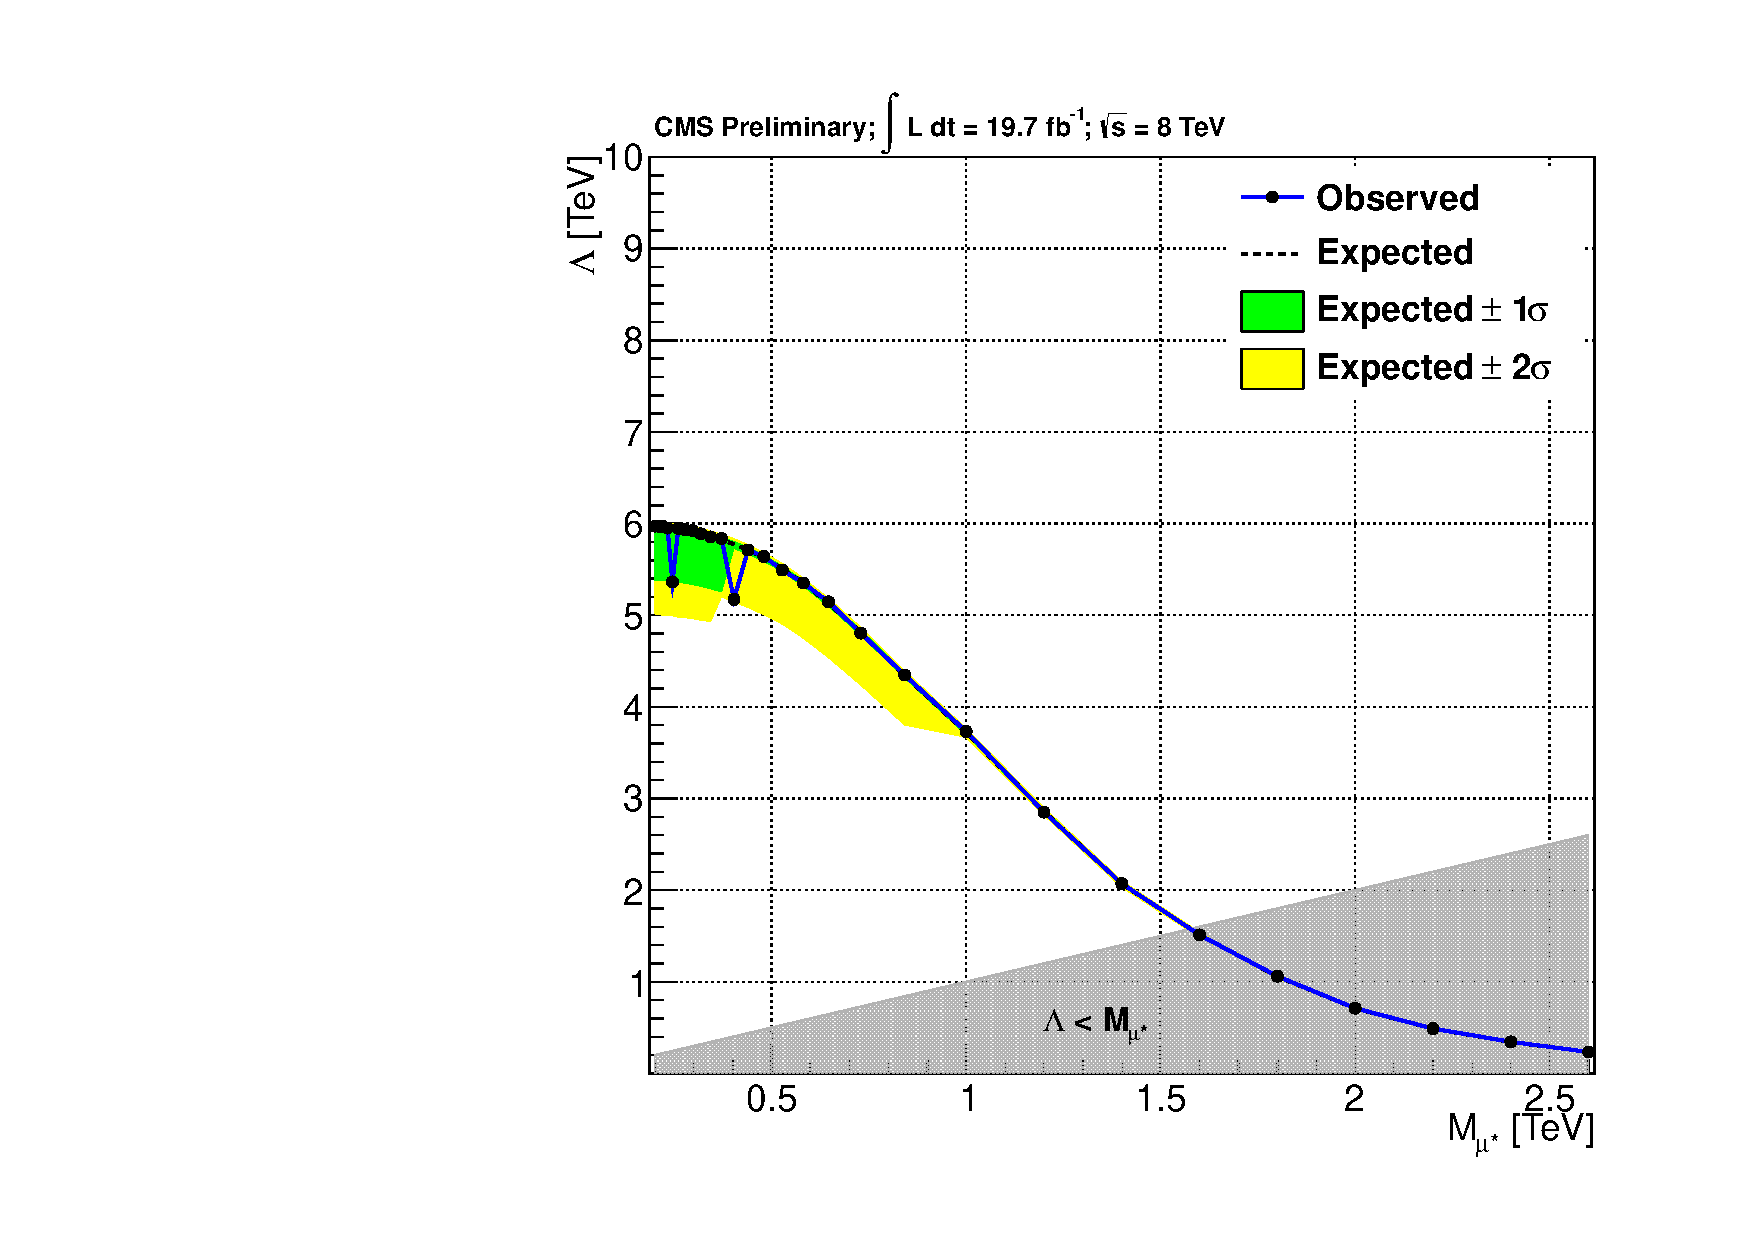
\includegraphics[width=0.48\textwidth]{plot/limit_lambda_2mu2e.pdf}
\end{center}
\caption{\label{fig:limit2mu2e}Cross section and $\Lambda$ limit for $\mu\mu^{*} \rightarrow 2\mu2e$.}
\end{figure}

\subsection{Limits for excited leptons $e^{*}$}

For excited electrons, the same limits as for the excited muons search has been calculated. Fig. \ref{fig:limit4e} and \ref{fig:limit2e2mu} show the cross section limits and the limits on the compositeness scale for $e^{*}\rightarrow 4e$ and $ee^{*} \rightarrow 2e2\mu$. Here, both channels exclud masses up to 1.60 TeV for $\Lambda = M_{e^{*}}$. 

\begin{figure}[hp!]
\begin{center}
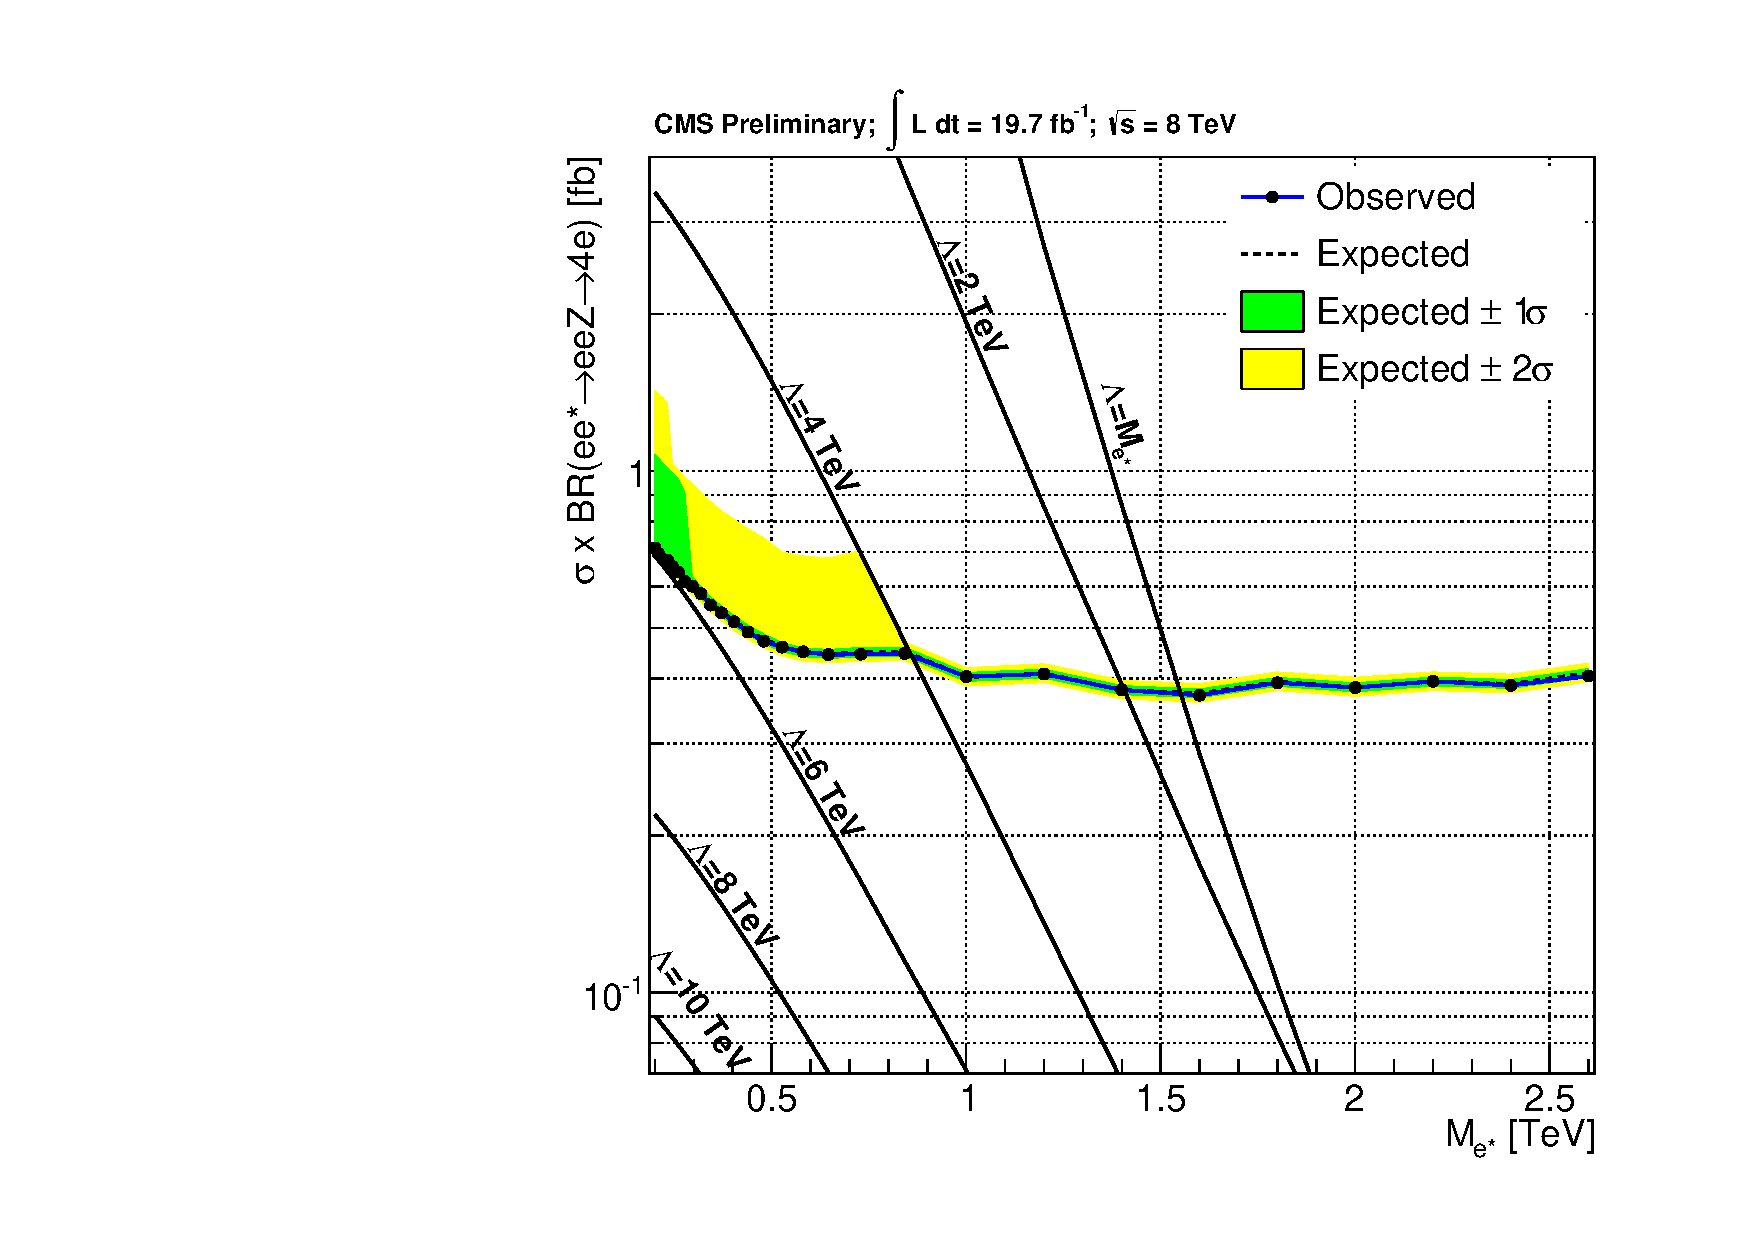
\includegraphics[width=0.48\textwidth]{plot/limit_4e.pdf}
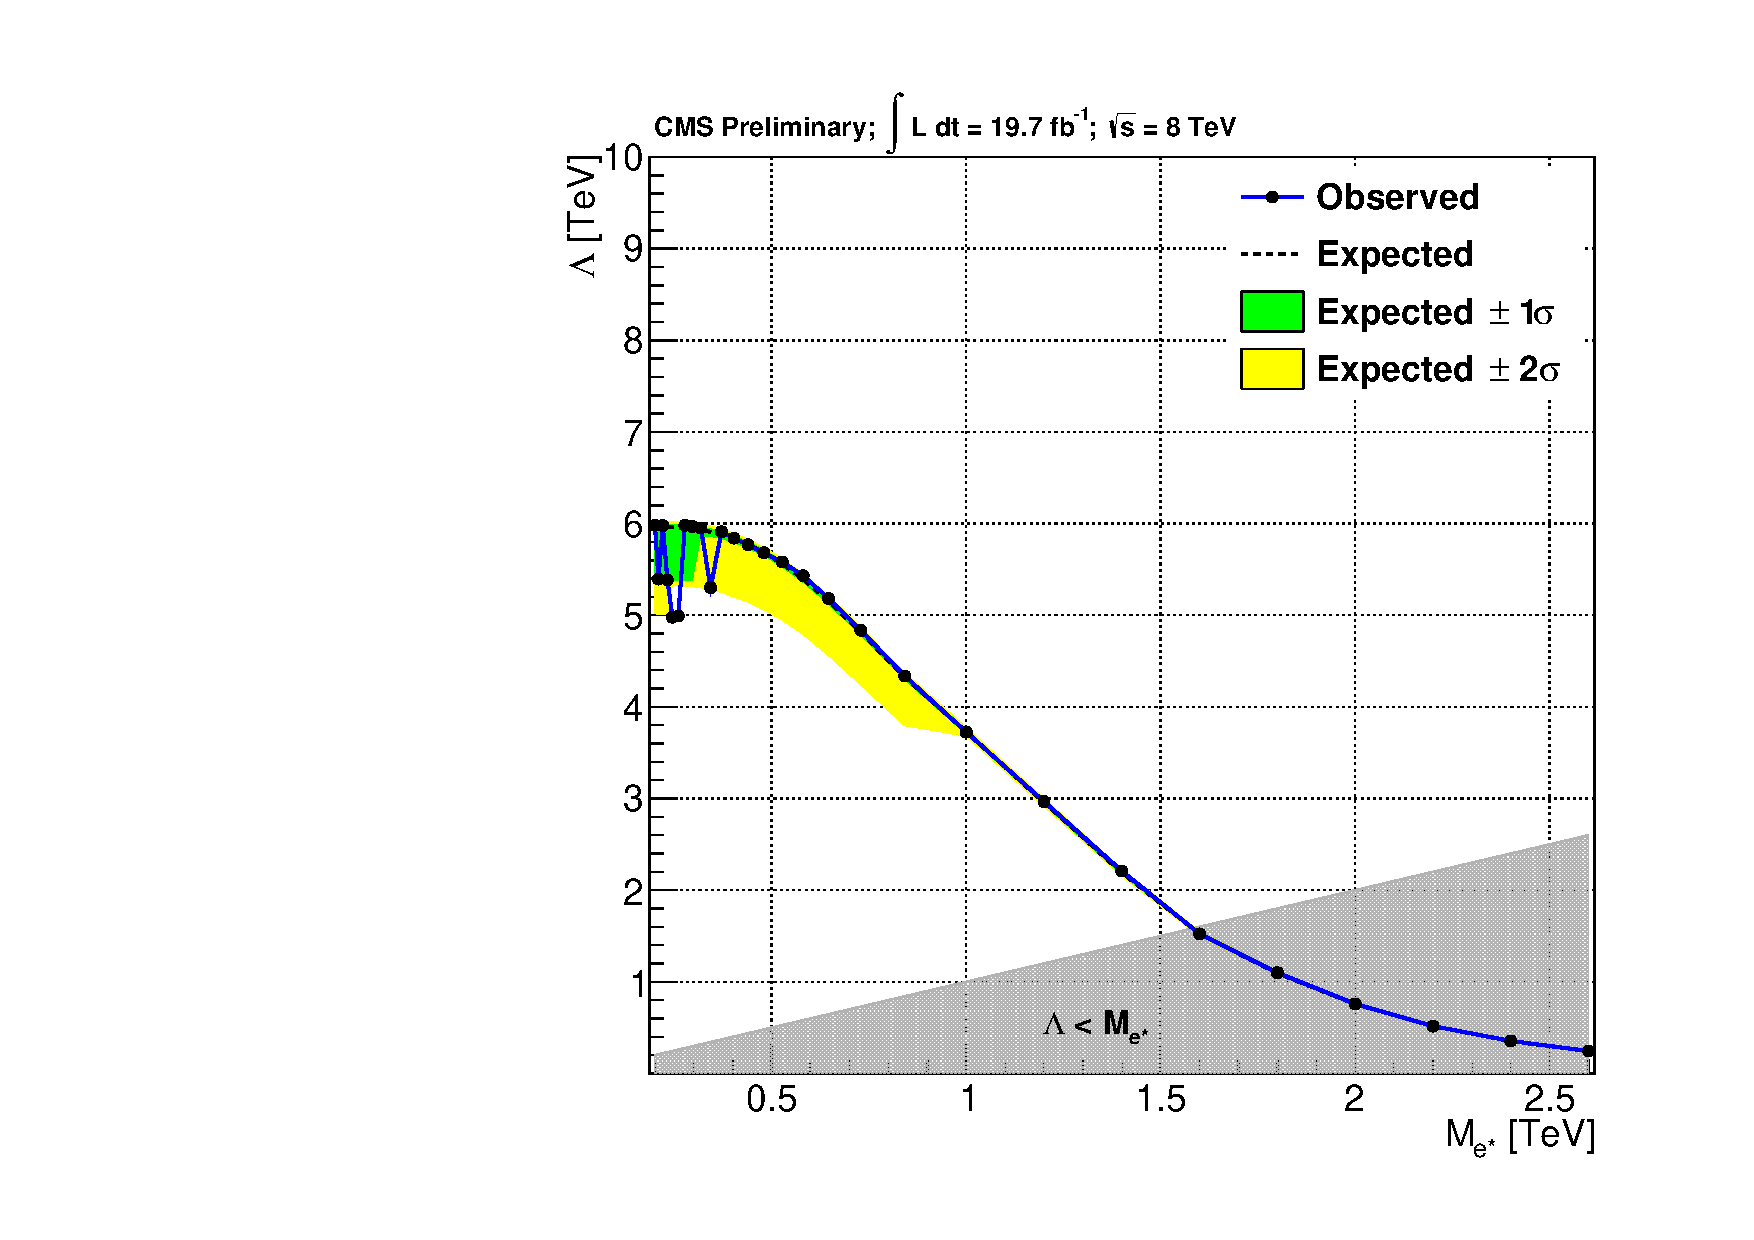
\includegraphics[width=0.48\textwidth]{plot/limit_lambda_2e2mu.pdf}
\end{center}
\caption{\label{fig:limit4e}Cross section and $\Lambda$ limit for $e e^{*} \rightarrow 4e$.}
\end{figure}

\begin{figure}[hp!]
\begin{center}
\includegraphics[width=0.48\textwidth]{plot/limit_2e2mu.pdf}
\includegraphics[width=0.48\textwidth]{plot/limit_lambda_2e2mu.pdf}
\end{center}
\caption{\label{fig:limit2e2mu}Cross section and $\Lambda$ limit for $e e^{*} \rightarrow 2e 2\mu$.}
\end{figure}

Depending on the limits of both channels, a combination has been done. This combination leads to an exclusion limit of 1.75 TeV for excited muons from Fig. \ref{fig:limitmustar}. The limit on excited electrons can be set to 1.7 TeV for $\Lambda = M_{e^{*}}$ as shown in \ref{fig:limitestar}. In all cases, the expected and observed limits are close to each other.

\begin{figure}[hp!]
\begin{center}
\includegraphics[width=0.48\textwidth]{plot/limit_combined_mustar.pdf}
\includegraphics[width=0.48\textwidth]{plot/limit_lambda_combined_mustar.pdf}
\end{center}
\caption{\label{fig:limitmustar}Combined cross section and $\Lambda$ limit for $\mu\mu^{*} \rightarrow 4l$.}
\end{figure}

\begin{figure}[hp!]
\begin{center}
\includegraphics[width=0.48\textwidth]{plot/limit_combined_estar.pdf}
\includegraphics[width=0.48\textwidth]{plot/limit_lambda_combined_estar.pdf}
\end{center}
\caption{\label{fig:limitestar}Combined cross section and $\Lambda$ limit for $e e^{*} \rightarrow 4l$.}
\end{figure}

The limit plots show some striking features. Looking at Fig. \ref{fig:limit4mu} to \ref{fig:limitestar} it can be seen that on the one hand, the error bands are mostly asymmetric around the median expected limit. On the other hand, the $1\sigma$- and sometimes also the $2\sigma$-band drop to a value very close to the dashed line of the median expected limit. Both effects have the same reason which is the low background expectation of below one event in the search regions (comp. Tab. \ref{tab:LShape2} - \ref{tab:LShape4}). During the limit computation, repeatedly toy-experiments are diced. When the background expectation is low, those are manly varied in the upper direction as it is not possible to reach under zero. Thus the asymetric error bands can be explained. When the background expectation becomes even lower as in the high mass search regions, the limit calculation is not able to iterate higher intger event assumptions and one after another, first the $1\sigma$- and later on also the $2\sigma$-quantile drop into the $0$-event assumption resulting in the very narrow error bands.

\section{Conclusion}
For the first time, a search for excited electrons and muons is performed in the channels with four leptons in the final states using pp collision data at $\sqrt{s} = 8 TeV$. No evidence of new physics is observed. Combining the respective two search channels, excited electrons with $M_{e^{∗}} < 1.70 TeV$ and excited muons with $M_{\mu^{∗}} < 1.75 TeV$ are excluded for the compositeness scale equals to the excited lepton mass ($M_{l^{*}} = \Lambda$).


\newpage


\appendix
%\bibliography{auto_generated}
%% This defines the bibliography file (main.bib) and the bibliography style.
%% If you want to create a bibliography file by hand, change the contents of
%% this file to a `thebibliography' environment.  For more information 
%% see section 4.3 of the LaTeX manual.
\begin{singlespace}
\bibliography{main}
\bibliographystyle{plain}
\end{singlespace}

\end{linenumbers}
\end{document}

